\documentclass{report}
\usepackage[utf8]{inputenc}
\usepackage[italian]{babel}
\usepackage{hyperref}
\usepackage[top=2.2cm, bottom=2.2cm, right= 2.5cm, left=2.5cm]{geometry}
\usepackage{amsmath, amsthm, amssymb, mathtools}
\usepackage{enumitem}
\usepackage{physics}
\usepackage{empheq, bm}
\usepackage{graphicx}
\usepackage{wrapfig}
\usepackage{subfig}
\usepackage{float}
\usepackage{verbatim}
\usepackage{upgreek}
\usepackage[dvipsnames]{xcolor}
\newcommand{\virgolette}[1]{``#1''}
\usepackage{soul}
\newcommand{\figref}[1]{figura \ref{#1}}
\newcommand{\tabref}[1]{tabella \ref{#1}}
\renewcommand{\eqref}[1]{equazione \ref{#1}}
\hypersetup
   {
   %bookmarks=true,         % show bookmarks bar?
    unicode=false,          % non-Latin characters in Acrobat’s bookmarks
    pdftoolbar=true,        % show Acrobat’s toolbar?
    pdfmenubar=true,       % show Acrobat’s menu?
    pdffitwindow=false,     % window fit to page when opened
    pdfstartview={FitH},    % fits the width of the page to the window
    pdftitle={Appunti di fisica biomedica-sanitaria},    % title
    pdfauthor={Simone Chiarella},     % author
    pdfsubject={Fisica biomedica-sanitaria},   % subject of the document
    pdfcreator={Simone Chiarella},   % creator of the document
   %pdfproducer={Producer}, % producer of the document
   %pdfkeywords={keyword1, key2, key3}, % list of keywords
    pdfnewwindow=false,      % links in new PDF window
    colorlinks=true,       % false: boxed links; true: colored links
    linkcolor=blue,          % color of internal links (change box color with linkbordercolor)
    citecolor=red,        % color of links to bibliography
    filecolor=magenta,      % color of file links
    urlcolor=cyan,           % color of external links
   %urlbordercolor={1 1 1}  % color of border around links
   }
\numberwithin{equation}{section}
\numberwithin{figure}{section}
\DeclareMathOperator{\sen}{sen}
\DeclareMathOperator{\senc}{senc}
\renewcommand{\thefootnote}{\fnsymbol{footnote}}
\renewcommand{\Vec}{\bm}
\addto{\captionsitalian}{\renewcommand{\abstractname}{}}
%\renewcommand*\figurename{Fig.\@}
%\renewcommand*\tablename{Tab.\@}

\title{Appunti dal corso di\\\vspace{10 pt} \textsc{\huge Elementi di Fisica Biomedica-Sanitaria}}
\author{Simone Chiarella}
\date{23 Settembre 2021}

\begin{document}
\maketitle
\shipout\hbox{}

\begin{abstract}
\large{Nel presente documento ho voluto raccogliere i contenuti del corso di \virgolette{Elementi di fisica biomedica-sanitaria}, tenuto nell'ambito del corso di laurea in Fisica dell'Università di Bologna durante l'a.a. 2020/2021. La trattazione degli argomenti contenuti in questa dispensa cerca di essere il più essenziale possibile, a volte eliminando alcune piccole parti da me ritenute \virgolette{eccessive} per una trattazione di questo livello e comunque non indispensabili ai fini del superamento dell'esame, anche con ottimi voti. Allo stesso tempo, con lo scopo di rendere più chiara la spiegazione di alcuni argomenti, gli appunti presi durante le lezioni e i seminari sono stati integrati con informazioni aggiuntive reperite da siti specializzati, libri di testo e tesi di laurea; si tratta comunque di informazioni di base che non necessitano di essere accompagnate da fonte, considerato anche il carattere didattico e interno di questo documento. Le immagini utilizzate sono state reperite nella stragrande maggioranza dei casi dalle diapositive presentate durante le lezioni e in nessun caso sono state realizzate da me.\\
Spero che il mio lavoro possa tornare utile al lettore di questo scritto.\\

\hspace{350 pt} Simone Chiarella}
\end{abstract}
\shipout\hbox{}

\tableofcontents

\chapter{Risonanza magnetica nucleare}

\section{Caratteri generali}
La risonanza magnetica nucleare (NMR) è un fenomeno fisico che coinvolge nuclei atomici con spin diverso da zero ed è caratterizzato da energie molto basse; i nuclei coinvolti nella maggior parte delle applicazioni sono nuclei di $\mathrm{^1H}$ (protoni), soprattutto quelli contenuti nelle molecole d'acqua, e tali nuclei hanno una frequenza di risonanza di 42,6\,MHz, la quale cade nel range delle poco energetiche onde radio. Per questo motivo, il segnale proveniente dalla risonanza dei nuclei viene rivelato in competizione con il rumore termico e la NMR è considerata, in generale, una tecnica d'indagine poco sensibile e caratterizzata da un basso rapporto segnale/rumore. La NMR, per questo motivo, viene utilizzata nelle situazioni in cui non è richiesto un gran livello di dettagli dell'immagine; in compenso, è una poco invasiva e abbastanza versatile perché multiparametrica, ossia l'intensità del segnale è pesata su diversi parametri che la rendono utilizzabile in diverse situazioni, sia in ambito diagnostico sia di ricerca scientifica.

\section{Scoperta del fenomeno}
L'esperimento che gettò le basi per lo sviluppo della NMR fu l'esperimento di Stern e Gerlach del 1921. I due scienziati fecero passare un fascio di atomi di argento attraverso un gradiente di campo magnetico e all'uscita il fascio risultò diviso in due. Poiché gli atomi di argento hanno un elettrone spaiato, si arrivò alla conclusione che il momento magnetico dell'elettrone spaiato può assumere due diversi valori. Ulteriori sviluppi portarono alla conclusione che ogni nucleo ha spin intero o semintero.

Un primo vero esperimento sulla risonanza magnetica fu quello di Rabi nel 1939 e illustrato nella \figref{fig:rabi}, in cui un fascio molecolare veniva fatto passare attraverso due magneti (A e B) che generavano due gradienti di campo magnetico opposto. La deflessione generata sul fascio dai due magneti è uguale e contraria, ma se si inserisce un terzo magnete (C) fra i due magneti originari, il quale genera un campo magnetico uniforme oscillante con la giusta frequenza (la frequenza di risonanza delle molecole del fascio), il fascio defletterà vistosamente. 

\begin{figure}[htp]
    \centering
    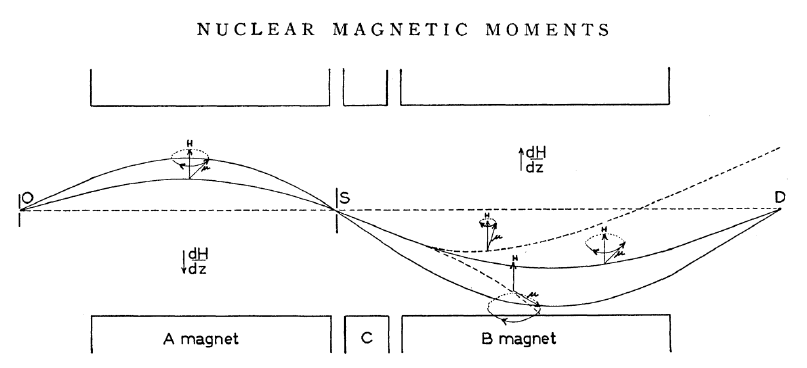
\includegraphics[scale=0.6]{rabi.png}
    \caption{\textit{Rappresentazione grafica dell'esperimento di Rabi del 1939}.}
    \label{fig:rabi}
\end{figure}

Attualmente, con il termine NMR ci si riferisce a fenomeni che differiscono da quelli osservati da Rabi per due motivi:
\begin{itemize}[label=$-$]
    \item l'effetto sui momenti magnetici è ottenuto impiegando campi a radiofrequenza;
    \item viene utilizzata materia condensata anziché fasci di atomi.
\end{itemize}
I primi due veri esperimenti di NMR furono quelli di Purcell e Bloch del 1946, condotti indipendentemente e contestualmente, rispettivamente su un solido (la paraffina) e su un liquido (l'acqua).

\section{Funzionamento e principi fisici}
Affinché si manifesti il fenomeno, il primo passo da fare è applicare un campo magnetico alla materia d'interesse, in modo da indurre una polarizzazione negli spin dei nuclei e orientarli tutti nello stesso verso; questo effetto si può ottenere in maniera più efficace se ci si trova a basse temperature, in modo che l'agitazione termica non influisca più di tanto. La polarizzazione degli spin avrà come conseguenza il manifestarsi di una grandezza macroscopica: la magnetizzazione. Per poterla rivelare, si applica un secondo campo magnetico, perpendicolare al primo e oscillante con frequenza circa uguale alla frequenza di risonanza dei nuclei che vogliamo eccitare. A questo punto, quando il sistema è eccitato, si spegne il secondo campo magnetico e, tramite un'apposita strumentazione hardware (ad esempio, una bobina ricetrasmittente), si studiano le radiazioni emesse dai nuclei eccitati, misurando i vari tempi di rilassamento, finché il sistema non sarà tornato alla condizione di equilibrio.

Vediamo ora quali sono i principi e le leggi fisiche dietro la risonanza magnetica nucleare. Come detto, i nuclei possono assumere valori del momento angolare di spin interi o seminteri. La presenza di uno spin diverso da zero fornisce i nuclei di un momento magnetico:
\begin{equation}
    \Vec{\mu} = \gamma_\mathrm{n} \bigg( \frac{\mathrm{h}}{2\uppi} \bigg) \Vec{I}\,,
\end{equation}
dove $\gamma_\mathrm{n}$ è il rapporto giromagnetico per il nucleo e $\Vec{I}$ è il momento angolare di spin. Esiste un metodo molto semplice per capire se un nucleo può essere utilizzato per svolgere NMR oppure no, e si basa sul numero di massa \textit{A} e sul numero atomico \textit{Z} del nucleo stesso:
\begin{itemize}[label=$-$]
    \item se \textit{A} e \textit{Z} sono pari, allora $\Vec{I}=0$, $\Vec{\mu}=0$ e non sarà possibile fare NMR ($\mathrm{^{12}C}$, $\mathrm{^{16}O}$);
    \item se \textit{A} è pari e \textit{Z} è dispari, allora $\Vec{I}$ ha modulo intero, $\Vec{\mu}$ è non nullo e sarà possibile fare NMR ($\mathrm{^2H}$, $\mathrm{^{14}N}$);
    \item se \textit{A} è dispari, allora $\Vec{I}$ ha modulo semintero, $\Vec{\mu}$ è non nullo e sarà possibile fare NMR ($\mathrm{^1H}$, $\mathrm{^{13}C}$, $\mathrm{^{23}Na}$).
\end{itemize}
Nella \figref{fig:iso} è possibile vedere i principali isotopi impiegabili in biomedicina che possono essere soggetti a NMR. Salta subito all'occhio il notevole rapporto giromagnetico del nucleo di idrogeno, il che giustifica il suo ampio utilizzo  per NMR in ambito clinico, in quanto un elevato rapporto giromagnetico produce un elevato momento magnetico del nucleo e restituisce un segnale più intenso. Gli isotopi con spin uguale a 1 non sono utilizzabili in ambito clinico perché richiedono tecniche molto avanzate. Sempre in ambito clinico, non trova impiego neanche il $\mathrm{^{19}F}$, ma viene utilizzato per lo studio di diversi farmaci chemioterapici somministrati in fase di sperimentazione agli animali.

Il risultato di una osservazione della componente \textit{z} del momento angolare $\Vec{I}$ di un singolo nucleo in uno stato di base è un numero \textit{m} intero o semintero compreso tra \textit{I} e \textit{-I}: \textit{m}, quindi, potrà assumere $2I+1$ valori. Di conseguenza, si avranno $2I+1$ valori anche per la misura della componente \textit{z} del momento magnetico:
\begin{equation}
    \mu_z=\gamma_\mathrm{n} \hbar m\,.
\end{equation}
Se il nucleo è in uno stato che è la sovrapposizione di stati di base, il risultato di una misura di $\hat{I}_z$ è:
\begin{equation}
    \sum_m \abs{a_m}^2 m\,.
    \label{sum}
\end{equation}

\begin{wrapfigure}{R}{0.55\textwidth}
    \centering
    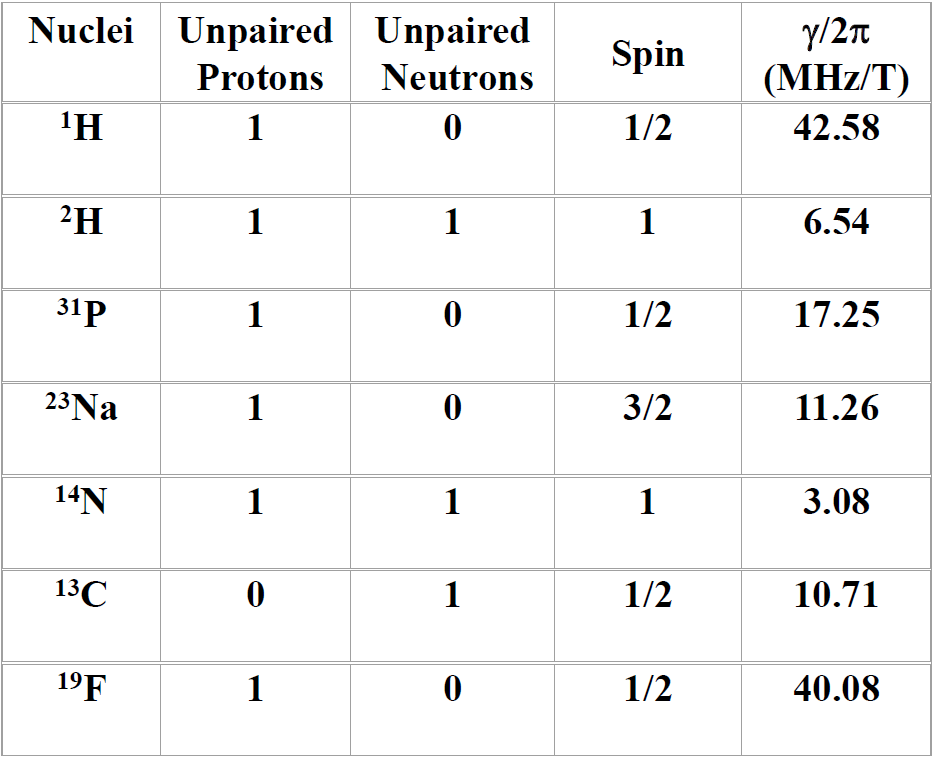
\includegraphics[width=0.5\textwidth]{iso.png}
    \caption{\textit{Isotopi impiegabili per NMR in biomedicina}.}
    \label{fig:iso}
\end{wrapfigure}

\noindent Per un singolo nucleo, il significato dell'\eqref{sum} è che la misura ha la probabilità $\abs{a_m}^2$ di restituire il risultato \textit{m}. Se, invece, abbiamo un gran numero di nuclei identici, la somma rappresenta la media degli \textit{m} pesati sulle probabilità $\abs{a_m}^2$. Da un punto di vista energetico, nel caso dello spin l'energia è espressa dall'operatore hamiltoniano:
\vspace{4 pt}
\begin{equation}
    \hat{H}=-\gamma \hbar \hat{I}_z B_0\,,
    \label{h}
\end{equation}
dove $B_0$ è il modulo del campo magnetico costante. Il campo magnetico dà luogo all'effetto Zeeman, cioè alla separazione dei livelli energetici, i quali avranno energia definita dagli autovalori dell'operatore hamiltoniano:
\vspace{4 pt}
\begin{equation}
    E_m=-\gamma \hbar m B_0\,.
\end{equation}
Per il nucleo di idrogeno $I=\frac{1}{2}$, quindi $m=\pm \frac{1}{2}$ e si avranno due livelli energetici con differenza di energia pari a $\gamma \hbar B_0$. Si dimostra, per $I=\frac{1}{2}$, che:
\begin{equation}
    \langle \Psi|I_x|\Psi \rangle=\frac{1}{2} \Big(\abs{a_{\frac{1}{2}}^* a_{-\frac{1}{2}}}-\abs{a_{\frac{1}{2}} a_{-\frac{1}{2}}^*} \Big)= \frac{1}{2} \Big(\abs{a_{\frac{1}{2}}}^2-\abs{a_{-\frac{1}{2}}}^2 \Big)\,.
    \label{psi}
\end{equation}
La quantità tra parentesi nell'\eqref{psi} riflette la coerenza di fase fra i due stati di spin e si dice che descrive il grado di \textit{single quantum coherence} dell'insieme. Il risultato può essere interpretato dicendo che il valore di aspettazione medio è determinato dalla differenza di popolazione fra i due livelli energetici. In condizioni di equilibrio tale differenza è nulla e determinata dalla distribuzione di Boltzmann:
\begin{equation}
    |a_{\pm \frac{1}{2}}|^2 = \frac{\exp{\pm \dfrac{\hbar \gamma B_0}{2\mathrm{k_B}T}}}{\exp{-\dfrac{\hbar \gamma B_0}{2\mathrm{k_B}T}}+\exp{\dfrac{\hbar \gamma B_0}{2\mathrm{k_B}T}}}\,.
\end{equation}
La grandezza fisica macroscopica osservabile, alla fine, sarà:
\begin{equation}
    \Vec{M}=N \gamma \hbar \big( \langle I_x \rangle \Vec{i} + \langle I_y \rangle \Vec{j} + \langle I_z \rangle \Vec{k} \big)\,,
\end{equation}
dove \textit{N} è il numero degli spin; all'equilibrio termico esiste una magnetizzazione longitudinale diretta come il campo magnetico, ma non c'è coerenza tra gli spin, ragion per cui la magnetizzazione trasversale sarà nulla.\\
In un sistema di nuclei, per un generico valore di \textit{I}, essi si disporranno sui $2I+1$ livelli energetici occupando prima quelli a energia più bassa. La densità di occupazione segue la seguente legge:
\begin{equation}
    \frac{n_{m-1}}{n_m}=\exp{-\frac{\hbar \omega_0}{\mathrm{k_B}T}} \,.
\end{equation}
Per $\mathrm{^1H}$ a temperatura ambiente e alla frequenza $\nu_0 = 100$\,MHz, si ha $\mathrm{k_B}T \gg \hbar \omega_0$: in tal caso, la differenza di popolazione è proporzionale all'intensità del campo magnetico e la magnetizzazione segue la legge di Curie:
\begin{equation}
    \Vec{M}_0=N \frac{\gamma^2 \hbar^2 I(I+1)}{3\mathrm{k_B}T}\Vec{B}_0 \,.
\end{equation}
Quando il sistema di nuclei assorbe energia, la magnetizzazione nucleare di equilibrio viene perturbata: tutte le informazioni sui nuclei, compreso il segnale che dà luogo a MRI, ci pervengono dall'evoluzione del sistema nel suo ritorno all'equilibrio. Nel caso dei nuclei di $\mathrm{^1H}$, la legge che regola il fenomeno di variazione della magnetizzazione è:
\begin{equation}
    \Vec{M}_0=\frac{N \gamma \hbar \mu}{2\mathrm{k_B}T}\Vec{B}_0 = N\,\frac{\gamma^2 \hbar^2}{4\mathrm{k_B}T}\Vec{B}_0 \,.
\end{equation}

\subsection{Precessione di Larmor}
Per comprendere al meglio l'evoluzione del sistema durante l'eccitazione, è necessario introdurre il fenomeno quantistico noto come \textbf{precessione di Larmor}, che si manifesta quando si applica un campo magnetico esterno a un atomo. In particolare, se i nuclei atomici sono dotati di momento magnetico, questi eseguiranno dei moti di precessione (a mo' di trottola) attorno alla direzione del campo magnetico esterno. Se indichiamo con $\Vec{M}$ il momento meccanico responsabile della precessione e con $\Vec{S}$ il momento angolare, allora vale:
\begin{equation}
    \Vec{M}=\frac{\mathrm{d}\Vec{S}}{\mathrm{d}t}=\Vec{\mu}\wedge\Vec{B}_0\,.
\end{equation}
Poiché $\Vec{\mu}=\gamma \Vec{S}$, allora:
\begin{equation}
    \frac{\mathrm{d}\Vec{\mu}}{\mathrm{d}t}=\Vec{\mu}\wedge\gamma\Vec{B}_0\,.
\end{equation}
Definiamo $\omega=\gamma B_0$, dove $B_0$ è il modulo del campo magnetico esterno, e infine otteniamo la \textbf{frequenza di Larmor} (o frequenza di risonanza):
\begin{equation}
    \boxed{\nu=\frac{\omega}{2\uppi}=\frac{\gamma B_0}{2\uppi}}
    \label{larmor}
\end{equation}

\begin{figure}[htp]
\centering
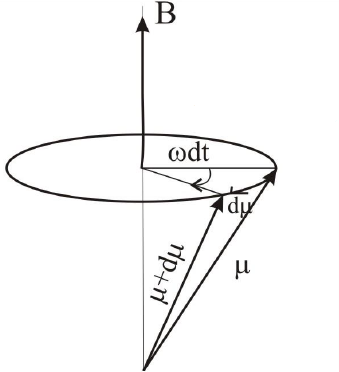
\includegraphics[scale=0.77]{larmor.png}\quad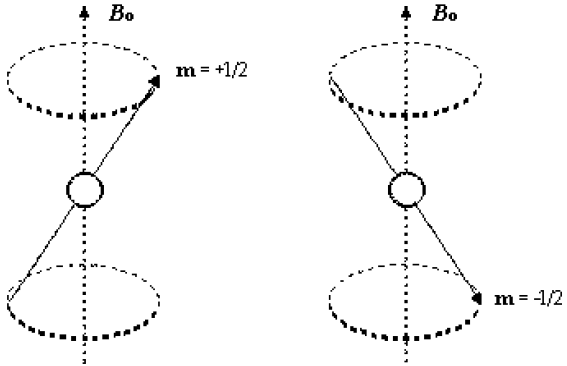
\includegraphics[scale=0.78]{precessione.png}
\caption{\label{fig:larmor} \textit{Rappresentazione grafica della precessione di Larmor}.}
\end{figure}

La precessione di Larmor trova riscontro in meccanica quantistica già nell'equazione di Schrödinger:
\begin{equation}
    \mathrm{ih}\frac{\partial}{\partial t}|\Psi(t)\rangle=\hat{H}|\Psi(t)\rangle\,.
\end{equation}
Se \textit{\^H} è costante, si ha:
\begin{equation}
    |\Psi(t)\rangle=U(t)|\Psi(0)\rangle\,,
\end{equation}
dove $U(t)=\exp{-\mathrm{i}Ht/\hbar}$. Ricordando l'\eqref{h}, si ottiene:
\begin{equation}
    U(t)=\mathrm{e}^{\mathrm{i}\gamma B_0 I_z t}\,,
\end{equation}
cioè l'evoluzione del sistema consiste nella rotazione in senso orario di un angolo $\gamma B_0 t$ attorno a \textit{z}; in presenza di un campo magnetico tutti gli stati precedono alla frequenza di Larmor data dall'\eqref{larmor}. Se invece di un nucleo si estende il ragionamento a un sistema di nuclei, non parleremo più dei singoli momento angolare $\Vec{S}$ e momento magnetico $\Vec{\mu}$ del nucleo che precede attorno alla direzione del campo magnetico, ma piuttosto ci si concentra sul momento angolare macroscopico $\Vec{J}$ e sulla magnetizzazione $\Vec{M}=\gamma \Vec{J}$ che precede attorno alla direzione del campo magnetico esterno.

\begin{wrapfigure}{R}{0.5\textwidth}
    \centering
    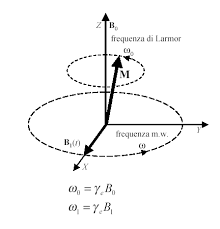
\includegraphics[width=0.35\textwidth]{b1.png}
    \caption{\textit{Rappresentazione delle grandezze fisiche in gioco nella NMR}.}
    \label{fig:b1}
\end{wrapfigure}

Tutti gli effetti visti finora (effetto Zeeman, comparsa della magnetizzazione, precessione di Larmor) sono conseguenze del primo campo magnetico costante $\Vec{B}_0$, ma, come accennato, per eccitare il sistema abbiamo bisogno di un secondo campo magnetico $\Vec{B}_1$, perpendicolare a $\Vec{B}_0$, che ruota attorno all'asse \textit{z} (si veda la \figref{fig:b1}) con frequenza pari alla frequenza di Larmor. Per effetto dell'applicazione di $\Vec{B}_1$, la direzione della magnetizzazione non esegue più solo una precessione attorno a $\Vec{B}_0$ ma varia anche di un angolo di nutazione che dipende dal tempo di applicazione di $\Vec{B}_1$:
\begin{equation}
    \alpha = \gamma B_1 t\,.
\end{equation}
In pratica, l'angolo di nutazione aumenta fin quando la magnetizzazione si porta dall'asse \textit{z} al piano \textit{xy} ($\alpha = 90$°) oppure dall'asse \textit{z} all'asse \textit{-z} ($\alpha = 180$°).

\subsection{Rilassamento}
Come già accennato, è il ritorno della magnetizzazione all'equilibrio il fenomeno che ci permette di poter ottenere informazioni sul sistema ed, eventualmente, produrre immagini (MRI). Tale processo è definito \textbf{rilassamento} e consiste nel ritorno della componente longitudinale della magnetizzazione al valore massimo, contestualmente all'annullamento della componente trasversale. Chiaramente il sistema ha bisogno di tempo per poter completare il rilassamento, come insegna l'esperienza di Gorter del 1942. Gorter, ancora prima di Purcell e Bloch, voleva rivelare l'assorbimento di energia da parte di nuclei $\mathrm{^1H}$ in acqua o di $\mathrm{^{19}F}$ in sostanze solide, ma non conoscendo il tempo di rilassamento longitudinale, che può essere anche di diversi secondi, si ritrovò a eccitare continuamente il sistema senza dargli il tempo necessario per poter tornare all'equilibrio; l'esperienza si rivelò un insuccesso. I rilassamenti delle due componenti seguono processi fisici differenti e sono entrambi descritti dalle equazioni di Bloch. Tratteremo separatamente i due rilassamenti concentrandoci proprio sui tempi di rilassamento.

\begin{wrapfigure}{R}{0.5\textwidth}
    \centering
    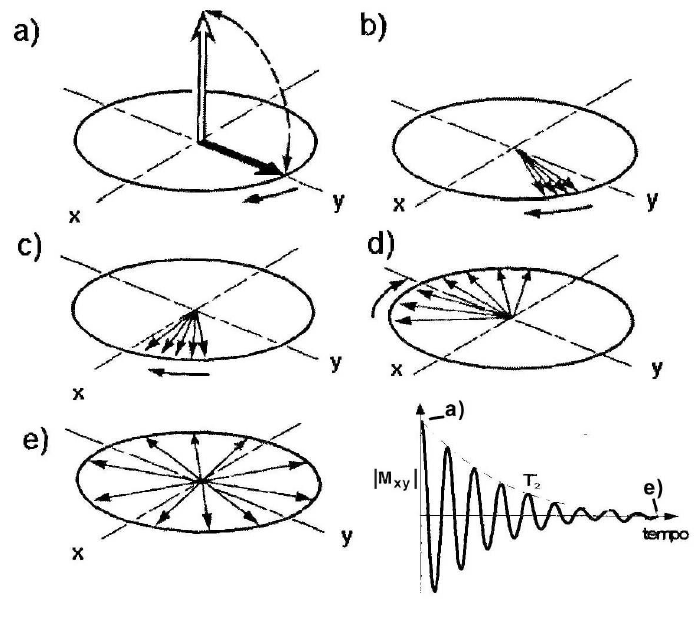
\includegraphics[width=0.45\textwidth]{trasversale.png}
    \caption{\textit{Rappresentazione grafica del rilassamento trasversale con particolare attenzione alla perdita di coerenza di fase}.}
    \label{fig:trasversale}
\end{wrapfigure}

Il \underline{rilassamento trasversale} è un processo entropico che si manifesta a causa della sfasatura dei gruppi di spin: se dopo aver applicato un angolo di nutazione di 90° alla magnetizzazione spegniamo il campo eccitante $\Vec{B}_1$, ci si potrebbe aspettare di primo acchito che i diversi spin che costituiscono la magnetizzazione continuino a precedere in senso orario attorno al campo $\Vec{B}_0$ tutti con la stessa frequenza, ma in realtà ciò non succede per due motivi:
\begin{enumerate}
    \item gli spin interagiscono fra loro, sfasandosi a vicenda;
    \item $\Vec{B}_0$ non è mai perfettamente omogeneo, perché viene deformato dalla materia stessa che attraversa, sia essa diamagnetica che, soprattutto, paramagnetica o ferromagnetica (come l'emoglobina, che contiene un atomo di ferro).
\end{enumerate}
Tutto ciò induce uno sfasamento nei diversi gruppi di spin che perdono la loro coerenza di fase (\figref{fig:trasversale}) e alla fine assumono tutti una propria frequenza diversa dalla frequenza di Larmor che possedevano inizialmente: di conseguenza, la magnetizzazione, che costituisce il segnale, tende a zero.

\noindent L'equazione di Bloch trasversale è:
\begin{equation}\label{bloch_trans}
    \frac{\mathrm{d}M_{xy}(t)}{\mathrm{d}t}=-\frac{M_{xy}(t)}{\mathrm{T_2}} \Rightarrow \boxed{M_{xy}(t)=M_{xy}(0)\,\mathrm{e}^{-\frac{t}{\mathrm{T_2}}}}
\end{equation}
In realtà, il $\mathrm{T_2}$ presente nell'equazione \ref{bloch_trans} è un $\mathrm{T_2^*}$, ovvero è il tempo di rilassamento trasversale che considera anche la non uniformità di $\Vec{B}_0$, mentre a noi interessa il vero $\mathrm{T_2}$, che è il tempo di rilassamento dovuto esclusivamente all'interazione reciproca tra spin. Occorre, dunque, elaborare un metodo per eliminare il contributo al rilassamento trasversale dovuto alla non uniformità del campo magnetico e calcolare $\mathrm{T_2}$: per riuscirci, ci si serve il concetto di eco.

\begin{figure}[htp]
    \centering
    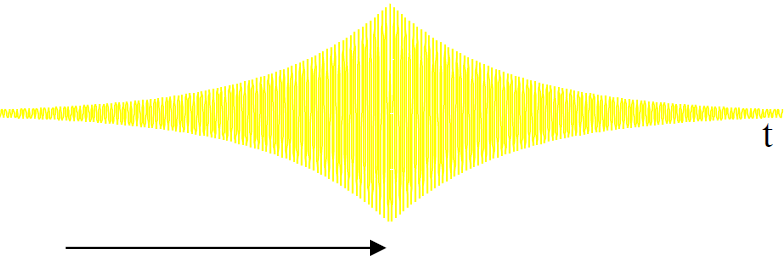
\includegraphics[scale=0.5]{eco.png}
    \caption{\textit{Esempio generico di un segnale eco}.}
    \label{fig:eco}
\end{figure}

\noindent In generale, l'eco è un qualsiasi segnale con ampiezza minima all'inizio, che aumenta col tempo fino a un massimo per poi diminuire di nuovo, come mostrato nella \figref{fig:eco}. Si ha un eco quando il segnale si sviluppa da un periodo di incoerenza a un periodo di coerenza. In particolare, la tipologia di eco utile ai fini della trattazione è la \textit{spin echo}, che possiamo fare emergere dal processo di rilassamento trasversale. Infatti, se dopo aver applicato alla magnetizzazione un impulso di 90° in fase di eccitazione, applichiamo (dopo un certo tempo, di cui si parlerà in seguito) un altro impulso di 180°, l'effetto che questo impulso avrà sugli spin sarà quello di ruotarli tutti di 180°, per l'appunto. Bisogna ricordarsi che gli spin hanno già perso la loro coerenza di fase quando l'impulso di 180° viene applicato, ma continuano a ruotare in senso orario nel piano \textit{xy} perpendicolare a $\Vec{B}_0$, e continueranno a farlo anche dopo l'inversione di 180°. Alla fine, dopo un lasso di tempo esattamente uguale al tempo che intercorre tra i due impulsi, gli spin riacquisteranno coerenza di fase e la magnetizzazione ritroverà l'intensità che possedeva prima che il processo entropico iniziasse. Definiamo il tempo di eco $T_\mathrm{E}$ come il tempo che separa l'applicazione del primo impulso dalla rifocalizzazione degli spin; di conseguenza il tempo che separa i due impulsi sarà pari a $\frac{T_\mathrm{E}}{2}$. Nella \figref{fig:riepilogo} si può vedere un riepilogo di tutto il processo. In particolare, si nota che se le interazioni fra spin fossero \virgolette{congelate} e si considerassero solo le disomogeneità del campo magnetico, i cui effetti sono resi nulli proprio dalla \textit{spin echo}, il segnale si rifocalizzerebbe completamente; se invece \virgolette{scongeliamo} le interazioni tra spin, il segnale sarà meno intenso di quello iniziale, come si può vedere dal picco dell'eco, che è più basso del picco iniziale del segnale.

\begin{figure}[htp]
    \centering
    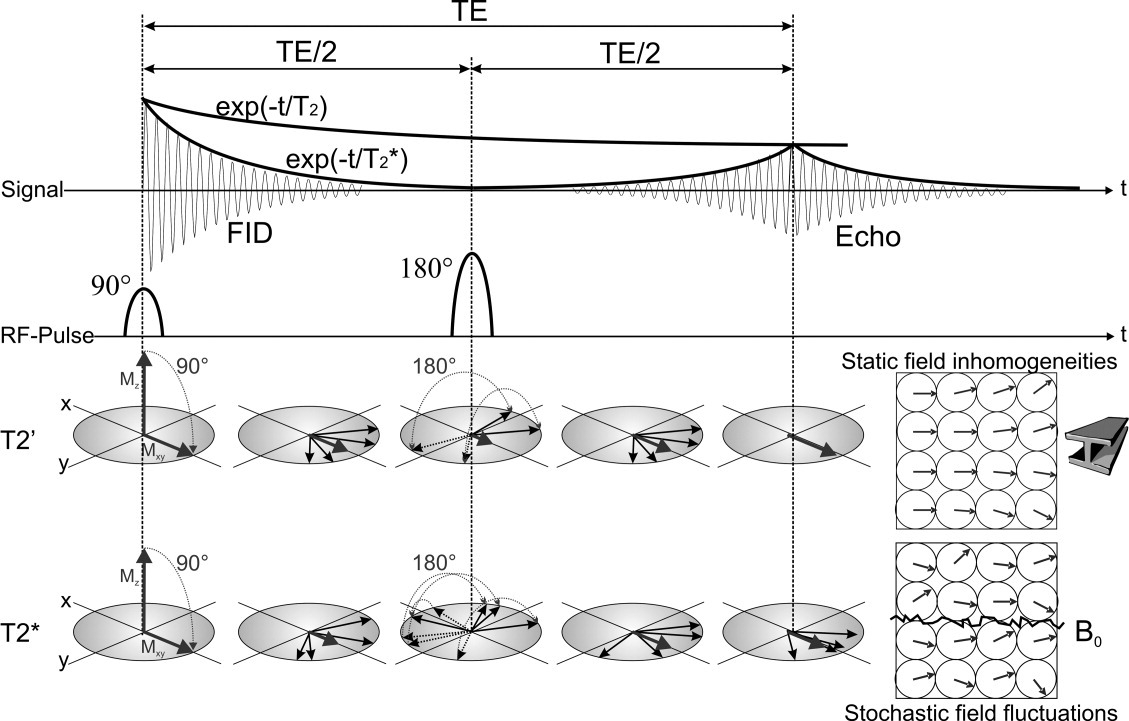
\includegraphics[scale=0.37]{riepilogo.jpg}
    \caption{\textit{Processo di rilassamento trasversale con sequenza spin echo}.}
    \label{fig:riepilogo}
\end{figure}

\begin{figure}[htp]
\centering
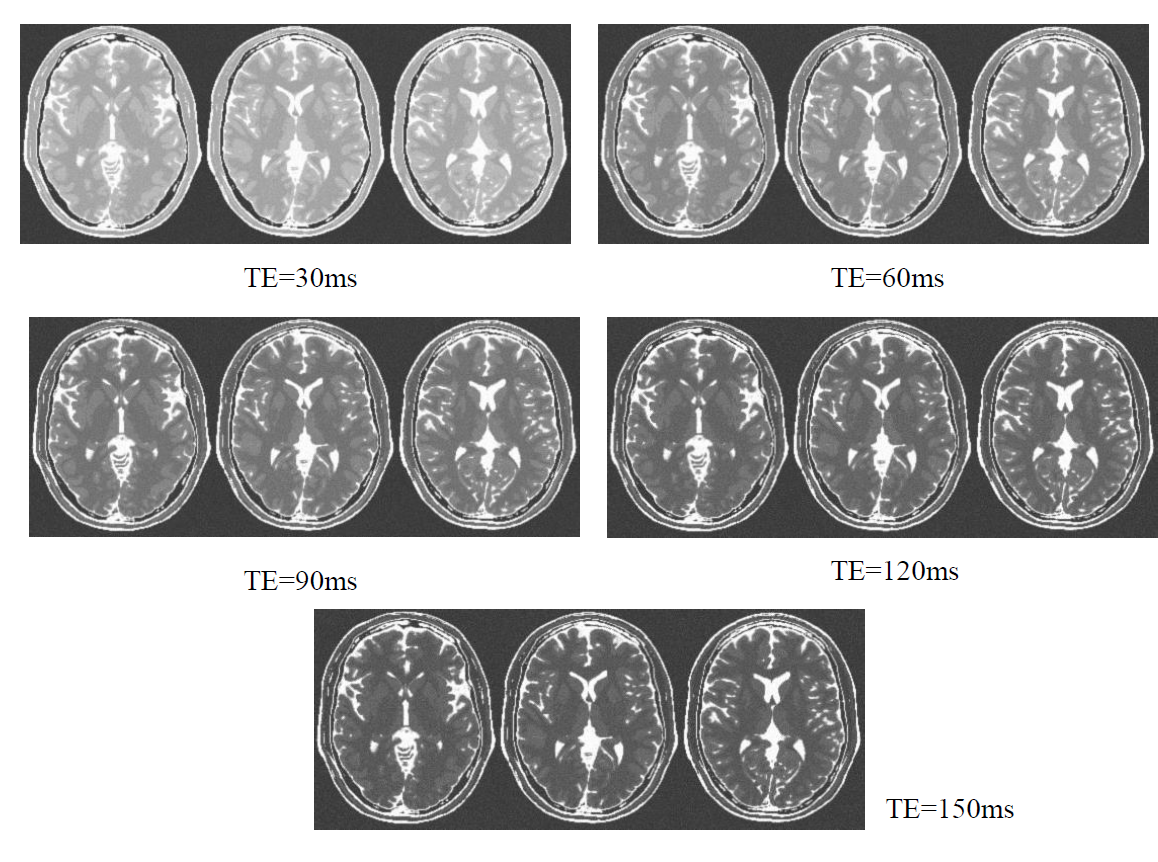
\includegraphics[scale=0.5]{tec.png}
\caption{\label{fig:tec} \textit{MRI trasversale di un cervello per diversi tempi di eco}.}
\end{figure}

\begin{wrapfigure}{R}{0.5\textwidth}
    \centering
    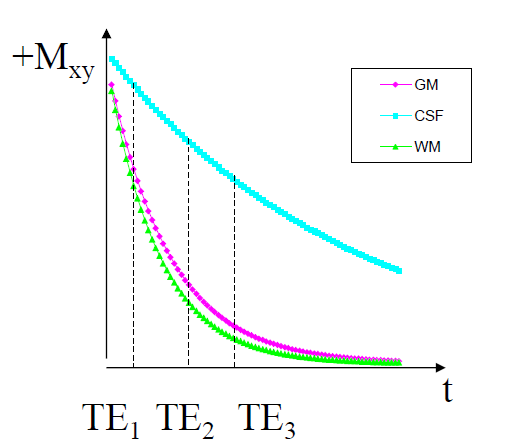
\includegraphics[width=0.45\textwidth]{te.png}
    \caption{\textit{Intensità del segnale in funzione del tempo di eco per rilassamento trasversale di materia grigia, materia bianca e liquido cefalorachidiano}.}
    \label{fig:te}
\end{wrapfigure}

Se non si considerano le disomogeneità che la materia analizzata induce nel campo, il tempo di rilassamento $\mathrm{T_2^*}$ coincide con $\mathrm{T_2}$; in altre parole, dopo un tempo $T_\mathrm{E}$ dall'applicazione del primo impulso, è come se il nostro sistema si sia evoluto con costante di tempo $\mathrm{T_2}$ invece che $\mathrm{T_2^*}$. Il tempo $T_\mathrm{E}$ che si sceglie, come pure la sequenza di impulsi, condiziona molto la qualità delle immagini. Ad esempio, nelle acquisizioni MRI riportate nella \figref{fig:tec}, si riesce a distinguere con grande facilità il liquor (che appare bianco) da tutto il resto, mentre la materia grigia e la materia bianca riescono vagamente a distinguersi solo per alcuni tempi di eco, segno che la sequenza di applicazione degli impulsi non è adeguata. La ragione del poco contrasto presente tra le due materie solide e dell'alto contrasto fra la parte liquida e quella solida del cervello è riscontrabile nella \figref{fig:te}; si può notare, infatti, come la sequenza di impulsi applicati riesca a separare molto bene il segnale proveniente dal liquido cefalorachidiano, che si mantiene piuttosto alto, da quelli provenienti dalla materia solida, che emettono un segnale di intensità quasi identica.

Un ultimo importante parametro per il rilassamento trasversale è il tempo di ripetizione $T_\mathrm{R}$, ossia il tempo che deve passare prima di poter rieccitare il sistema, in caso si desideri avere ulteriori informazioni sulla materia in esame. Si può dimostrare un'utile espressione per il modulo della magnetizzazione in funzione di $T_\mathrm{R}$ e $T_\mathrm{E}$:
\begin{equation}
    M(T_\mathrm{R},T_\mathrm{E})= M_0 \Big[1-\mathrm{e}^{-\frac{T_\mathrm{R}}{\mathrm{T_1}}} \Big(\mathrm{e}^{-\frac{T_\mathrm{E}}{2\mathrm{T_1}}}-1 \Big) \Big]\mathrm{e}^{-\frac{T_\mathrm{E}}{\mathrm{T_2}}}\,,
    \label{segnale}
\end{equation}
dove $\mathrm{T_1}$, come si vedrà tra un attimo, è il tempo di rilassamento longitudinale.
\newpage
Il \underline{rilassamento longitudinale} è un processo energetico che si manifesta a causa dello scambio di energia fra il sistema di spin, che ha assorbito energia, e il reticolo al quale tale energia viene ceduta: in pratica, quando il campo eccitante $\Vec{B}_1$ viene spento, la componente longitudinale della magnetizzazione ricompare e la magnetizzazione non fa altro che riportarsi in direzione parallela al campo $\Vec{B}_0$.\\
L'equazione di Bloch longitudinale è:
\begin{equation}
    \frac{\mathrm{d}M_z(t)}{\mathrm{d}t}=-\frac{M_z(t)-M_0}{\mathrm{T_1}} \Rightarrow \boxed{M_z(t)=M_z(0)\,\mathrm{e}^{-\frac{t}{\mathrm{T_1}}}+M_0 \Big(1-\mathrm{e}^{-\frac{t}{\mathrm{T_1}}} \Big)}
\end{equation}

\begin{wrapfigure}{R}{0.4\textwidth}
    \centering
    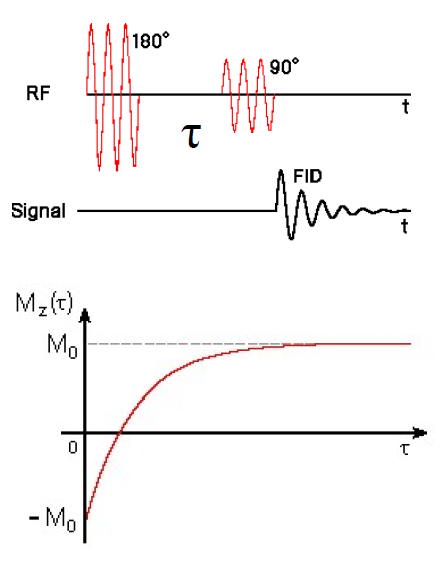
\includegraphics[width=0.35\textwidth]{long.png}
    \caption{\textit{Applicazione degli impulsi e modulo della magnetizzazione in funzione del tempo $\tau$ per rilassamento longitudinale}.}
    \label{fig:long}
\end{wrapfigure}

\noindent Come per il rilassamento trasversale, per calcolare $\mathrm{T_1}$ è sufficiente applicare una coppia di impulsi alla materia da indagare. Per eccitare il sistema si applica un primo impulso di 180°, in modo da ribaltare la magnetizzazione e portarla dal semiasse positivo di \textit{z} a quello negativo; un secondo impulso di 90°, applicato dopo un tempo $\tau$, servirà successivamente per avere informazioni sulla magnetizzazione longitudinale. In seguito al ribaltamento della magnetizzazione, come mostrato nella \figref{fig:long}, si avrà $M_z(0)=-M_0$ e, sostituendo nell'equazione di Bloch longitudinale si ottiene:
\begin{equation}
    M_z(\tau)=M_0 \Big(1-2\mathrm{e}^{-\frac{\tau}{\mathrm{T_1}}} \Big)\,.
    \label{Mz}
\end{equation}
Supponiamo di voler ottenere un'immagine MRI per un campione costituito da due tessuti diversi: il nostro scopo sarà mettere in evidenza uno di questi due tessuti, cercando di impostare i parametri in modo che l'altro non restituisca segnale o lo faccia debolmente rispetto al primo. L'equazione da considerare sarà semplicemente la somma di due equazioni dello stesso tipo dell'\eqref{Mz} per i due tessuti:
\begin{equation}
    S(\tau)=S_1 \Big(1-2\mathrm{e}^{-\frac{\tau}{\mathrm{T_{11}}}} \Big) + S_2 \Big(1-2\mathrm{e}^{-\frac{\tau}{\mathrm{T_{12}}}} \Big)\,.
\end{equation}
Poniamo uguale a zero il segnale del primo tessuto e otterremo il valore di $\tau$ che stiamo cercando:
\begin{equation}
    S_1 \Big(1-2\mathrm{e}^{-\frac{\tau}{\mathrm{T_{11}}}} \Big)=0 \hspace{3 pt} \Rightarrow \hspace{3 pt} 2\mathrm{e}^{-\frac{\tau}{\mathrm{T_{11}}}}=1 \hspace{3 pt} \Rightarrow \hspace{3 pt} \ln2=\frac{\tau}{\mathrm{T_{11}}} \hspace{3 pt} \Rightarrow \hspace{3 pt} \tau=\mathrm{T_{11}}\ln2\,.
    \label{tau}
\end{equation}
L'utilità dell'\eqref{tau} può essere compresa osservando la \figref{fig:flair}, la quale mostra due immagini ottenute con MRI e pesate in $\mathrm{T_2}$: l'immagine di sinistra mette in evidenza tessuti come meningi e liquor, mentre quella di destra mette in evidenza la materia cerebrale vera e propria. Per ottenerla è stata impiegata proprio l'\eqref{tau}: infatti, conoscendo $\mathrm{T_1}$ del tessuto che vogliamo oscurare ($\mathrm{T_1}=2000$\,ms) si può calcolare $\tau$, ovvero il tempo dopo il quale dovremo applicare il secondo impulso: $\tau = 2000\,\text{ms} \times \ln2 = 1400$\,ms.

\begin{figure}[htp]
\centering
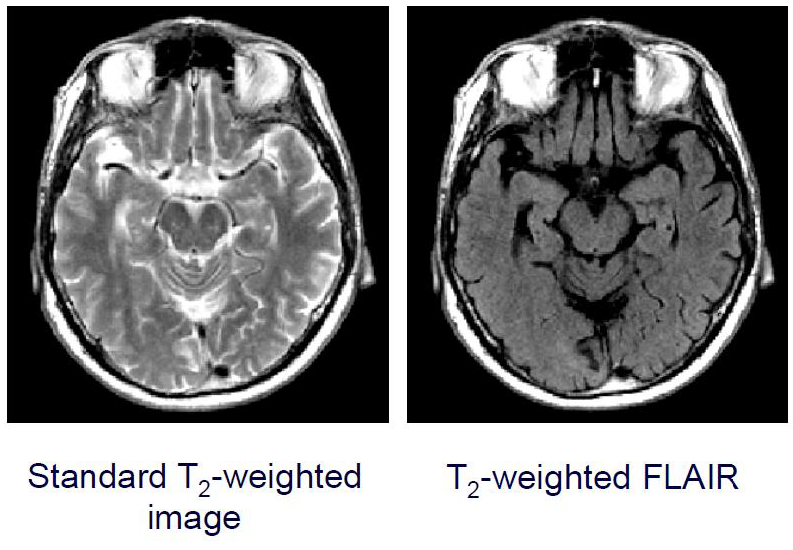
\includegraphics[scale=0.4]{flair.png}
\caption{\label{fig:flair} \textit{MRI pesato in $\mathrm{T_2}$ con tecniche diverse, in modo da mettere in evidenza tessuti differenti}.}
\end{figure}

Il segnale di un voxel (equivalente volumetrico del pixel) in MRI acquisito con sequenza \textit{spin echo} (SE) per un dato $\mathrm{M}_0$ è dato da:
\begin{equation}
    M(T_\mathrm{R},T_\mathrm{E})= \mathrm{M}_0 \Big[1-\mathrm{e}^{-\frac{T_\mathrm{R}}{\mathrm{T_1}}} \Big(2\mathrm{e}^{\frac{T_\mathrm{E}}{2\mathrm{T_1}}}-1 \Big) \Big]\mathrm{e}^{-\frac{T_\mathrm{E}}{\mathrm{T_2}}}\,,
    \label{trte}
\end{equation}
A partire dall'\eqref{trte} è già possibile capire, a grandi linee, il valore che è necessario assegnare ai parametri per ottenere un'immagine pesata in un modo piuttosto che in un altro. Facciamo quale esempio:
\begin{itemize}[label=$-$]
    \item per un'immagine pesata in densità di protoni dobbiamo rendere dominante $\mathrm{M_0}$, perciò bisognerà fare in modo che $\mathrm{e}^{-\frac{T_\mathrm{R}}{\mathrm{T_1}}}$ tenda a 0 e che $\mathrm{e}^{-\frac{T_\mathrm{E}}{\mathrm{T_2}}}$ tenda a 1, impostando $T_\mathrm{R} \geq 5\mathrm{T_1}$ e $T_\mathrm{E} \ll \mathrm{T_2}$;
    \item per un'immagine pesata in $\mathrm{T_2}$ dobbiamo rendere dominante $\mathrm{e}^{-\frac{T_\mathrm{E}}{\mathrm{T_2}}}$, perciò bisognerà fare in modo che $\mathrm{e}^{-\frac{T_\mathrm{R}}{\mathrm{T_1}}}$ tenda a 0, impostando $T_\mathrm{R} \geq 5\mathrm{T_1}$ e $T_\mathrm{E} \geq \mathrm{T_2}$;
    \item per un'immagine pesata in $\mathrm{T_1}$ dobbiamo rendere dominante $\mathrm{e}^{-\frac{T_\mathrm{R}}{\mathrm{T_1}}}$, perciò bisognerà fare in modo che $\mathrm{e}^{-\frac{T_\mathrm{E}}{\mathrm{T_2}}}$ tenda a 1, impostando $T_\mathrm{R} \leq \mathrm{T_1}$ e $T_\mathrm{E} \ll \mathrm{T_2}$.
\end{itemize}

Nella \figref{fig:uovo} possiamo vedere un esempio per comprendere meglio la correlazione fra i tempi di rilassamento e i contrasti fra i vari tessuti. Nell'acquisizione in densità di protoni si vede come il segnale proveniente dall'albume sia più intenso, segno che esso contiene più protoni rispetto al tuorlo. Nell'immagine pesata in $\mathrm{T_2}$, invece, l'albume emette più segnale del tuorlo, il che ci dice che il tempo di rilassamento trasversale dell'albume è più lungo di quello del tuorlo. Al contrario, come si evince dall'immagine pesata in $\mathrm{T_1}$, il tempo di rilassamento longitudinale del tuorlo è più lungo di quello dell'albume. In generale, i materiali liquidi sono caratterizzati da tempi di rilassamento più lunghi dei materiali solidi.

\begin{figure}[htp]
\centering
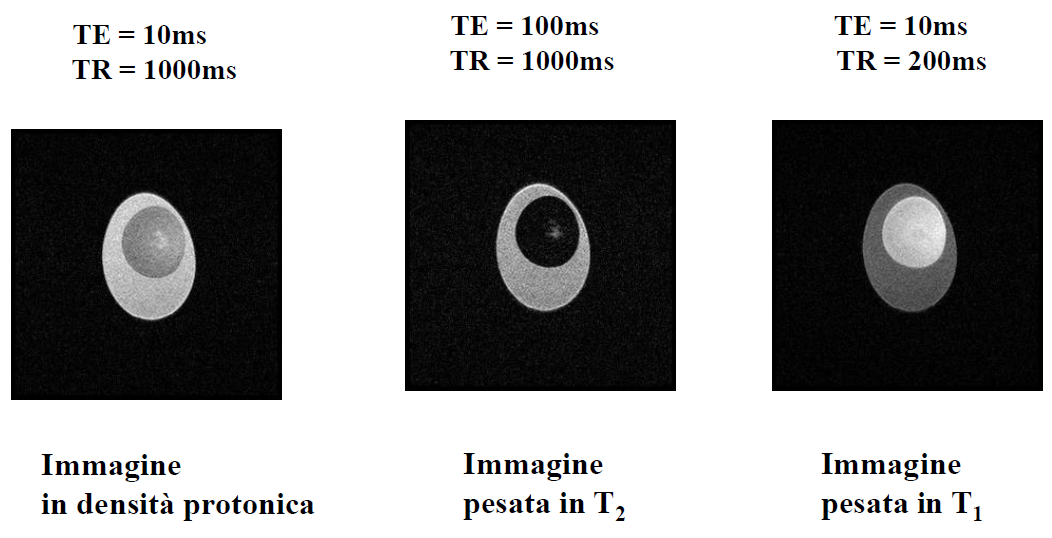
\includegraphics[scale=0.6]{uovo.png}
\caption{\label{fig:uovo} \textit{MRI di un uovo in pesature differenti}.}
\end{figure}

\section{Tomografia a NMR}
In questo capitolo ci si occuperà di come poter ricavare delle immagini con la tecnica della risonanza magnetica nucleare. In particolare, i due quesiti a cui ci si propone di rispondere sono i seguenti.
\begin{itemize}[label=$-$]
    \item Come ottenere delle immagini spazialmente risolte a partire da un segnale NMR che si riferisce all'intero campione?
    \item Come si riesce a ottenere una risoluzione spaziale anche di un millimetro o, in ambito non clinico, anche inferiore se la lunghezza d'onda della radiofrequenza utilizzata è più grande di diversi ordini di grandezza?
\end{itemize}
Innanzitutto, bisogna specificare che il segnale che proviene dalla diseccitazione del campione è costituito da un inviluppo di segnali a diverse frequenze, a causa delle differenze negli spin dei nuclei del campione. Per ricavare dal segnale acquisito la distribuzione di frequenze di Larmor dei nuclei (che chiameremo \textbf{proiezione}) è comodo usare l'analisi di Fourier. Questa ci permette di ricavare dei picchi di frequenze dall'inviluppo; l'intensità dei picchi rappresenta la quantità di nuclei che emettono radiazione di una certa frequenza.

\begin{figure}[htp]
\centering
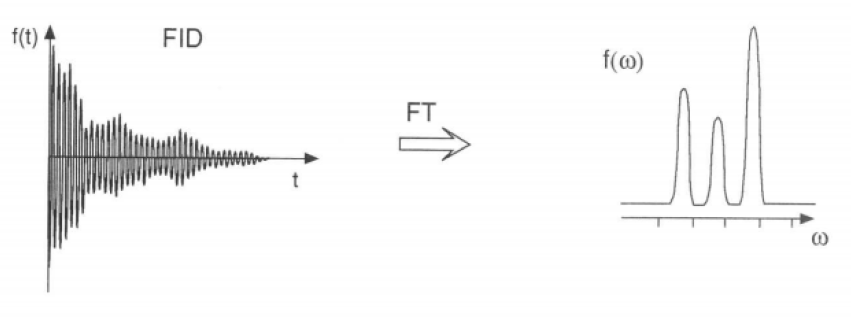
\includegraphics[scale=0.66]{fourier.png}
\caption{\label{fig:fourier} \textit{Effetto dell'applicazione della trasformazione di Fourier a un inviluppo}.}
\end{figure}

\subsection{Mappatura 2D}
Immaginiamo di avere tre provette piene d'acqua di volume diverso immerse in un campo magnetico uniforme. Poiché le provette sono riempite della stessa sostanza, la frequenza del segnale che emetteranno sarà identica e, sebbene l'intensità del segnale proveniente da ciascuna provetta sarà diversa (a causa del diverso numero di nuclei di idrogeno presente in ognuna di esse), alla fine non sarà possibile distinguere i singoli segnali. L'unica maniera possibile per distinguerli è fare in modo che la frequenza dei segnali emessi, ossia la frequenza di Larmor dei nuclei di idrogeno di ciascuna provetta, sia diversa. Per fare ciò, in base all'\eqref{larmor}, è necessario fare in modo che il campo magnetico applicato a ciascuna provetta sia diverso: in altre parole, è necessario applicare non un campo magnetico uniforme ma un gradiente di campo magnetico, come mostrato nella \figref{fig:gradiente}. Se il gradiente applicato è costante e diretto lungo \textit{x}, la formula per l'intensità del campo magnetico sarà:
\begin{equation}
    B_z(x)=B_z(0)+G_xx \hspace{2 pt}, \hspace{4 pt} G_x=\frac{\Delta B_z(x)}{\Delta x}=\mathrm{cost.}
\end{equation}
Di conseguenza, la frequenza di risonanza dei nuclei dipenderà linearmente dalla loro posizione lungo \textit{x}:
\begin{equation}
    \nu (x)= \frac{\gamma}{2\uppi}(B_z(0)+G_xx) \,.
\end{equation}

\begin{figure}[htp]
\centering
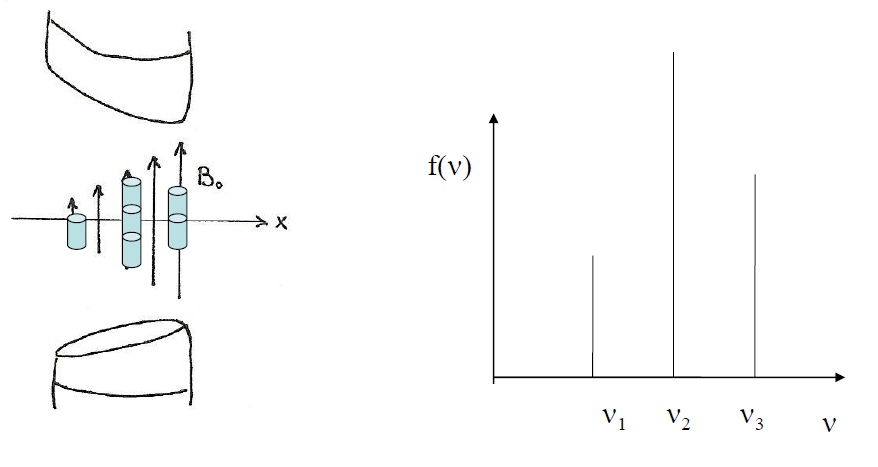
\includegraphics[scale=0.6]{gradiente.png}
\caption{\label{fig:gradiente} \textit{Gradiente da applicare a campioni della stessa sostanza per poter distinguere i diversi segnali}.}
\end{figure}

\noindent La tecnica appena illustrata è nota col nome di \textbf{zeugmatografia} ed è possibile riassumerla in quattro punti:
\begin{itemize}[label=$-$]
    \item assegnare a ciascun punto dell'asse \textit{x} un diverso valore del campo magnetico, che corrisponderà a una diversa frequenza di Larmor;
    \item analizzare il segnale NMR tramite analisi di Fourier per ottenere la proiezione lungo \textit{x};
    \item l'intensità del segnale a una certa frequenza risulterà proporzionale alla densità di nuclei di idrogeno in una certa posizione spaziale (in realtà l'immagine avrà sempre una pesatura in qualche parametro);
    \item per ottenere un'immagine spazialmente risolta occorrerà ripetere l'operazione lungo direzioni diverse, ottenendo varie proiezioni.
\end{itemize}

\begin{figure}[htp]
\centering
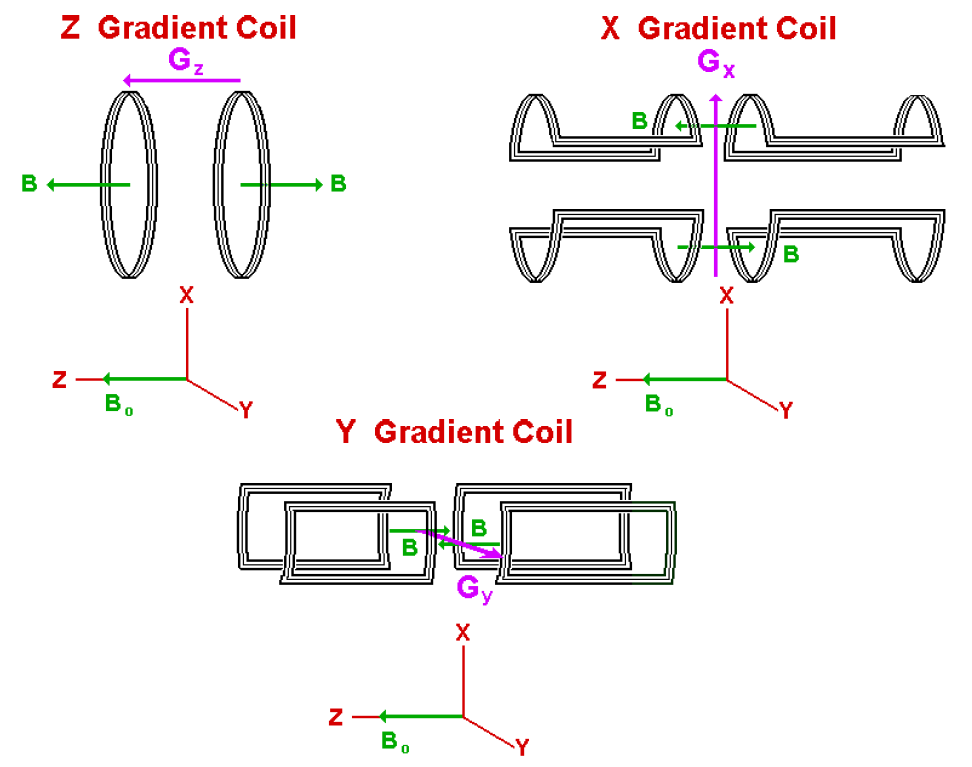
\includegraphics[scale=0.5]{bobine.png}
\caption{\label{fig:bobine} \textit{Bobine di gradiente per direzioni diverse}.}
\end{figure}

\subsection{Mappatura 3D}
Vediamo come si può estendere la tecnica appena esposta per la mappatura bidimensionale a una mappatura tridimensionale. Di fatto, bisogna selezionare il segnale di una sezione all'interno di un campione tridimensionale, ossia bisogna selezionare una fetta. Per fare ciò, non è necessario che il sistema hardware esegua nessun movimento meccanico, come succede per altre tecniche diagnostiche, ma è sufficiente applicare contemporaneamente tre gradienti lungo le tre dimensioni spaziali. È importante non fare confusione tra la direzione dei gradienti di campo e il campo stesso: bisogna ricordare che comunque si tratta di tre gradienti della stessa componente $B_z$ del campo magnetico, quindi, anche se i gradienti di campo sono diretti in tre direzioni diverse, il campo in sé sarà diretto come \textit{z}.
\begin{equation}\boxed{
    \begin{cases}
    G_x = \Delta B_z/\Delta x \\
    G_y = \Delta B_z/\Delta y \\
    G_z = \Delta B_z/\Delta z
    \end{cases}
    \Vec{G}=G_x\Vec{i}+G_y\Vec{j}+G_z\Vec{k}}
\end{equation}
Ciascuna terna $(G_x,G_y,G_z)$ individua una direzione nello spazio tale che:
\begin{itemize}[label=$-$]
    \item spostandosi lungo tale direzione, si ha la più rapida variazione di $B_z$;
    \item $B_z$ è costante sul piano perpendicolare a tale direzione.
\end{itemize}
In altre parole, la direzione del vettore gradiente individua un asse perpendicolare a sezioni del campione da esaminare, e su ciascuna sezione $B_z$ assume lo stesso valore, pur variando lungo la direzione stessa. Volendo fare un esempio, se si applica, come nell'immagine di sinistra della \figref{fig:mela}, un gradiente $G_r=\Delta B_z/\Delta r=15$\,mT/m, e assumendo che lo spessore della fetta sia $\Delta r=1$\,mm, si ha che la variazione del campo magnetico in quella fetta è $\Delta B_z=15\times10^{-6}$\,T = 0,15\,G. Le frequenze del segnale proveniente dalla fetta selezionata sono comprese in un intervallo $\Delta \nu$ = 46,2\,MHz/T $\times 15 \times 10^{-6}$\,T = 640\,Hz. Il modo privilegiato per selezionare un segnale emesso in un intervallo di frequenze preciso è quello di applicare al campione un impulso selettivo, cioè tale per cui la sua trasformata di Fourier sia una funzione rettangolare (immagine di destra della \figref{fig:mela}) limitata nel dominio di frequenze in questione. La funzione più utilizzata come impulso selettivo è il seno cardinale, definito come segue:
\[ \senc{x} =
   \begin{cases}
    \dfrac{\sen{x}}{x} & \quad \text{se } x\neq0 \\
    1                          & \quad \text{se } x=0 \,.
   \end{cases}
\]
In sintesi, l'introduzione del gradiente di campo magnetico è sufficiente solo per distinguere spazialmente le frequenze, ma per ricevere segnale esclusivamente dai punti spaziali, e quindi dalle frequenze, che ci interessano, è necessario che il campo $\Vec{B}_1$ abbia una forma ben precisa: quella della funzione $\senc{x}$.

\begin{figure}[htp]
\centering
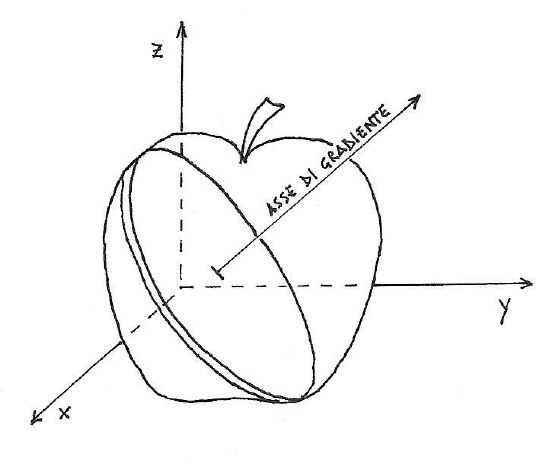
\includegraphics[scale=0.685]{mela.png}\quad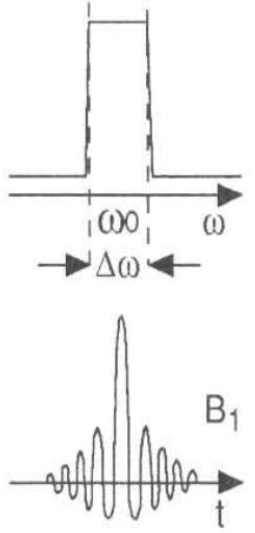
\includegraphics[scale=0.6]{sinc.png}
\caption{\label{fig:mela} \textit{A sinistra, raffigurazione di un gradiente di selezione di una fetta; a destra, andamenti della funzione \textnormal{senc}(t) e della sua trasformata di Fourier}.}
\end{figure}

\subsection{Metodo \textit{spin-warp}}
Il \textbf{metodo \textit{spin-warp}} è la più semplice sequenza per \textit{imaging} e consta delle seguenti cinque fasi.
\begin{enumerate}
    \item \emph{Applicazione di un impulso a radiofrequenza di 90°}: la sua forma è quella del seno cardinale e consiste in una breve e intensa cessione di energia.
    \item \emph{Attivazione del gradiente di selezione}: viene attivato contemporaneamente all'impulso del punto 1., in modo da selezionare una fetta del campione da esaminare, ed è diretto lungo \textit{z} (direzione di $\Vec{B}_0$).
    \item \emph{Attivazione del gradiente per la codifica di fase}: si attiva quando viene spento il gradiente di selezione, è diretto lungo \textit{y} e il suo compito è quello di far precedere gli spin sul piano \textit{xy} con frequenze diverse, a seconda delle posizioni dei nuclei lungo l'asse \textit{y}.
    \item \emph{Attivazione del gradiente per la codifica di frequenza}: si attiva quando viene spento il gradiente per la codifica di fase, è diretto lungo \textit{x} e il suo compito è quello di far precedere gli spin sul piano \textit{xy} con frequenze diverse, a seconda delle posizioni dei nuclei lungo l'asse \textit{x}.
    \item \emph{Ricezione del segnale}: avviene contestualmente al punto 4.
\end{enumerate}
Nell'immagine di sinistra della \figref{fig:k} sono raffigurate le diverse fasi. In pratica, quando viene spento il gradiente per la codifica di fase, gli spin riprenderanno a precedere tutti alla stessa frequenza, ma la fase di precessione di ogni gruppo di spin che condivide la stessa posizione lungo l'asse \textit{y} sarà ormai diversa da tutti gli altri gruppi. L'utilità del gradiente per la codifica di frequenza sarà quella di selezionare anch'esso dei gruppi di nuclei che condividono la stessa posizione lungo l'asse \textit{x}, e far precedere gli spin dei nuclei di ciascun gruppo con frequenza diversa dagli spin dei nuclei di tutti gli altri gruppi. Siccome esistono, però, già dei gruppi caratterizzati da fasi di precessione diverse e discriminati in base alla loro posizione lungo l'asse \textit{y}, quest'ulteriore differenziazione lungo l'asse \textit{x} fa in modo che lo spin di ogni singolo nucleo abbia una fase e una frequenza di precessione diverse da qualsiasi altro nucleo del campione. La sequenza \textit{spin-warp} viene di solito ripetuta 128 o 256 volte per poter raccogliere tutti i dati necessari per produrre un'immagine; ogni volta che la sequenza viene ripetuta l'intensità del gradiente per la codifica di fase cambia.
\vspace{- 7 pt}
\begin{figure}[htp]
\centering
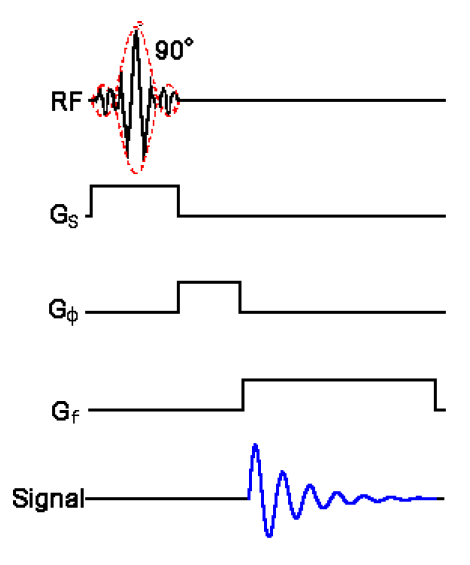
\includegraphics[scale=0.5]{sw.png}\quad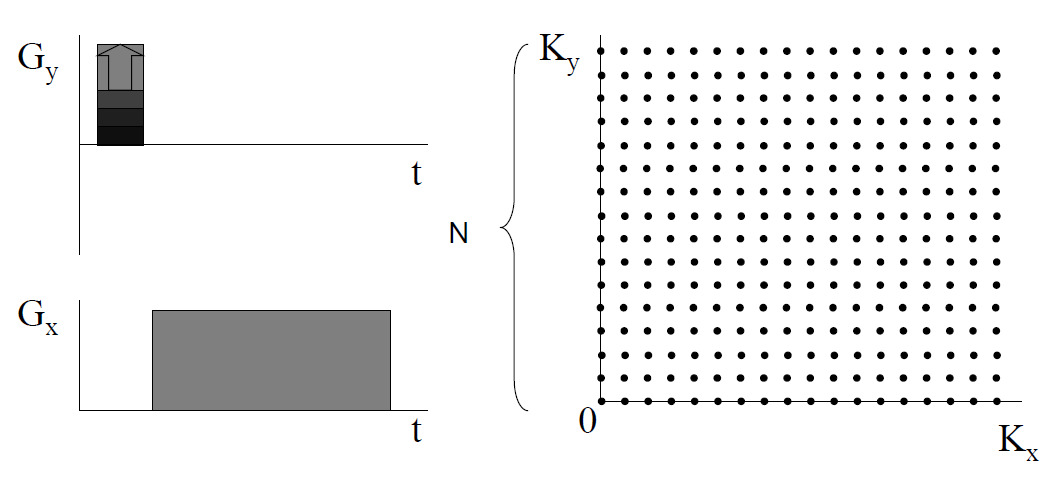
\includegraphics[scale=0.5]{k.png}
\caption{\label{fig:k} \textit{Da sinistra a destra: sequenza spin-warp con indicazione grafica della durata di ogni fase e riempimento dello spazio k al variare di $G_y$}.}
\end{figure}

\vspace{-12 pt}

\subsection{Codifica spaziale e campionamento} \label{1.4.4}
Per poter trattare la modalità di traduzione del segnale in pixel, è comodo introdurre il vettore d'onda:
\begin{equation}
    \Vec{k}=\gamma \Vec{G}t \,.
\end{equation}
Sperimentalmente, per ottenere la mappatura del piano si fanno variare $k_x=\gamma G_x t$ e $k_y=\gamma G_y t$, poiché la distribuzione spaziale dei pixel in un'immagine MRI è:
\begin{equation}
    \rho(x,y) \approx \iint S(k_x,k_y) \mathrm{e}^{\mathrm{i}(k_xx+k_yy)}\,\mathrm{d}k_x\,\mathrm{d}k_y\,.
\end{equation}
dove $S(k_x,k_y)$ è l'intensità del segnale. Si tratta, quindi, di far variare $k_x$ in \textit{M} modi e $k_y$ in \textit{N} modi, per campionare lo spazio \textit{k} con $M \times N$ punti e ricavare una mappatura della densità in $M \times N$ punti, cioè $M \times N$ pixel. In pratica, per ogni variazione del gradiente $G_y$, viene acquisita un’intera riga dello spazio \textit{k} lungo l’asse \textit{x} e, dopo \textit{N} acquisizioni, ognuna con $G_y$, lo spazio \textit{k} sarà totalmente riempito e l'immagine sarà completa, come mostrato sulla destra della \figref{fig:k}; il tempo totale di acquisizione è $T_R \times N$.

Nella \figref{fig:k2} si possono vedere delle interferenze nelle immagini di sinistra dovute a errori nell'acquisizione. Nelle immagini raffiguranti gli spazi \textit{k}, in corrispondenza delle frecce, sono presenti dei puntini troppo luminosi, che sono le cause delle interferenze. Ogni punto dello spazio \textit{k} rappresenta un’onda nell'immagine. Il livello di grigio del punto rappresenta l’ampiezza dell'onda nell'immagine, la distanza dall'origine è correlata alla frequenza e l’angolo alla fase. La sovrapposizione di tutte le onde rappresentate nello spazio \textit{k} con la loro ampiezza, frequenza e fase costituisce l’immagine. A riprova di ciò, come si vede in figura, più il punto è vicino all'origine, minore è la frequenza delle bande d'interferenza e i fronti d'onda sono perpendicolari al segmento che unisce il punto luminoso all'origine; in particolare, nell'ultima immagine le bande di interferenza sono così sottili che a stento si riescono a vedere, infatti il puntino luminoso nel corrispondente spazio \textit{k} è molto lontano dall'origine. Se l'interferenza si trova lontano dall'origine, si potrebbe scegliere di selezionare solo la parte centrale dello spazio \textit{k}, cioè il segnale a bassa frequenza. Questo permette di eliminare l'interferenza, ma l'immagine così ottenuta sarebbe poco risolta, come si può vedere nelle immagini di destra della \figref{fig:k2}, proprio perché le basse frequenze corrispondono a lunghezze d'onda elevate che sono in grado di riprodurre soltanto le grandi aree dell'immagine e gli ampi contrasti, ma non possono ricostruire i dettagli minuti. Al contrario, se si seleziona solo il segnale ad alta frequenza, nell'immagine che si otterrebbe sarebbero in evidenza i dettagli e i bordi degli oggetti, ma si perderebbe il contrasto.

\begin{figure}[htp]
\centering
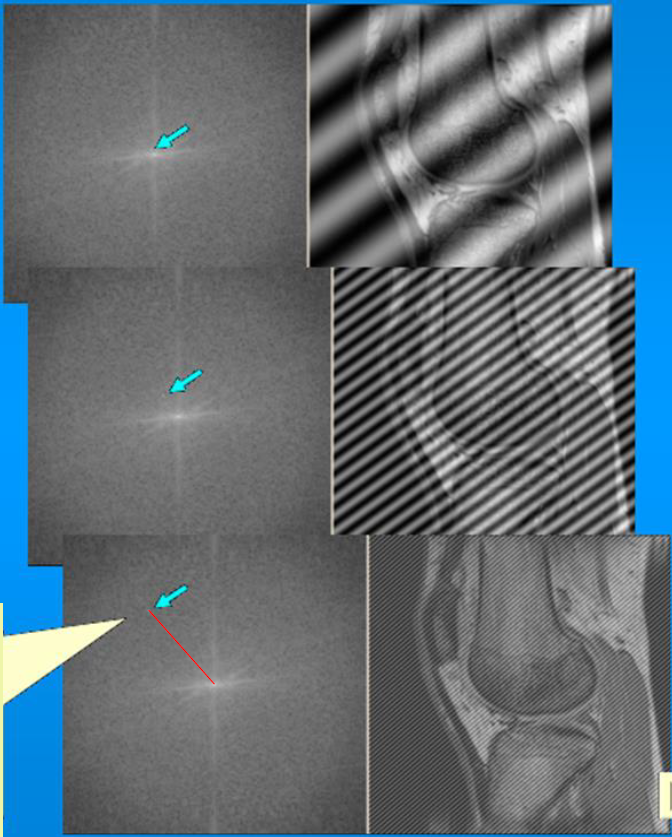
\includegraphics[scale=0.505]{k2.png}\quad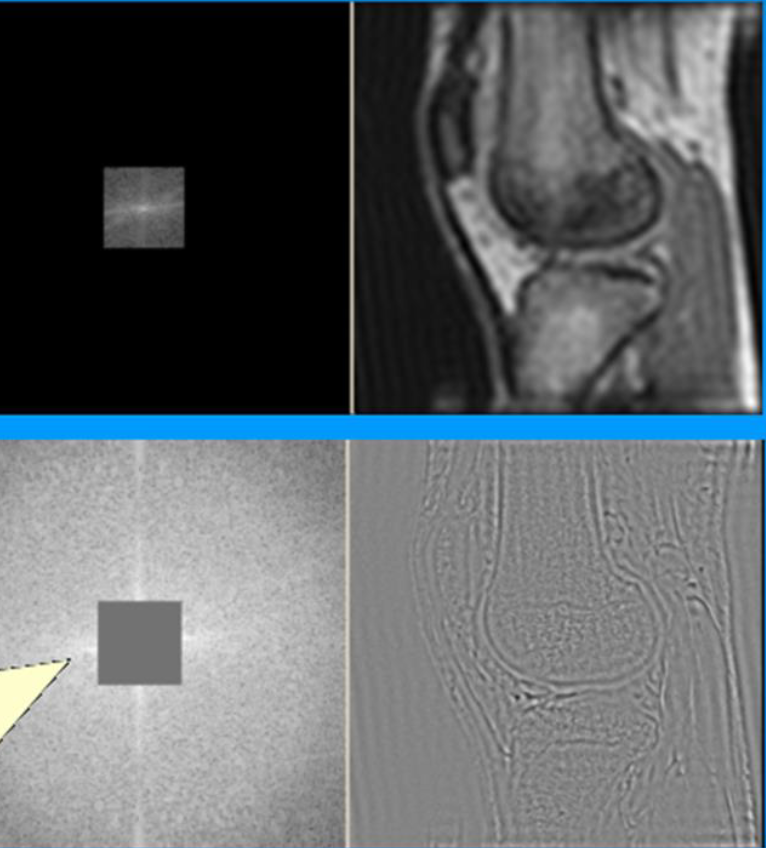
\includegraphics[scale=0.5]{k3.png}
\caption{\label{fig:k2} \textit{A sinistra, spazi k acquisiti con un'interferenza; a destra, selezione del segnale nello spazio k in base alla frequenza, con rispettive immagini}.}
\end{figure}

\vspace{-5 pt}

Rimane da discutere riguardo al campionamento del segnale, in particolare circa la frequenza di campionamento. Come mostrato nella \figref{fig:aliasing}, se non si campiona il segnale con la frequenza giusta può verificarsi il fenomeno dell'\textit{aliasing}, ossia un'ambiguità nel campionamento effettuato che non permette di dedurre la frequenza del segnale stesso. Se il campione da indagare è più piccolo dell'oggetto posto nello scanner, di cui il campione costituisce una parte, l'\textit{aliasing} si manifesta nell'immagine finale come una sovrapposizione, nel senso che le parti dell'oggetto al di fuori dell'area di \textit{imaging} vengono sovrapposte all'immagine che si vuole ottenere. Per evitare l'\textit{aliasing}, è necessario seguire il \textbf{teorema di Nyquist}, il quale afferma che per campionare un segnale senza perdita di informazione, bisogna adottare una frequenza di campionamento maggiore di almeno il doppio rispetto alla frequenza della massima componente spettrale del segnale. In questo caso, come si intuisce dall'immagine di destra della \figref{fig:aliasing}, la frequenza campionata sarà univoca.

\begin{figure}[htp]
\centering
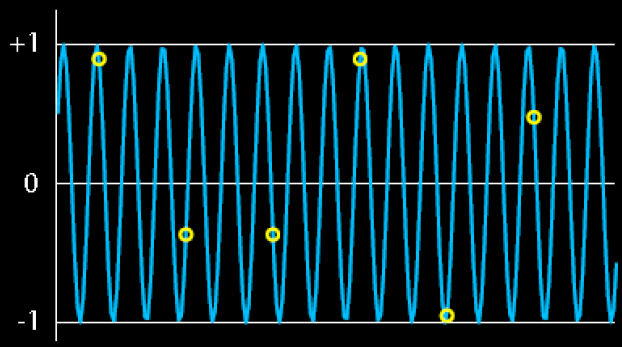
\includegraphics[scale=0.614]{aliasing.png}\quad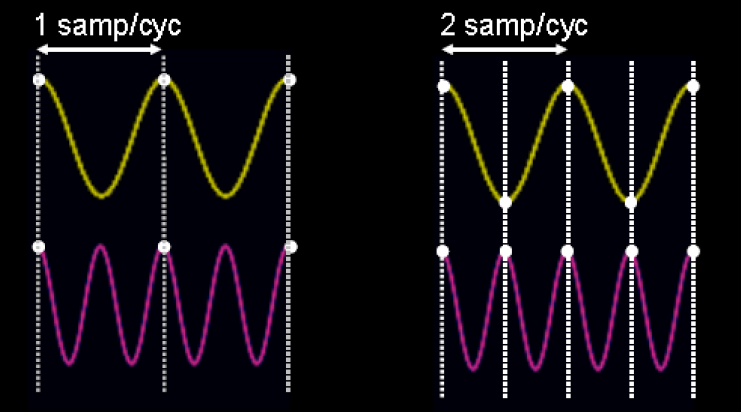
\includegraphics[scale=0.518]{nyquist.png}
\caption{\label{fig:aliasing} \textit{A sinistra, campionamento non adeguato che dà luogo ad aliasing; a destra, rimozione dell'ambiguità mediante frequenza di campionamento maggiore}.}
\end{figure}

\section{Spettroscopia di risonanza magnetica}
Se si esclude l'ambito sanitario, la spettroscopia è l'applicazione della risonanza magnetica più utilizzata: è impiegata in biologia per studi anche su cellule vive, in campo veterinario su animali vivi precedentemente anestetizzati, e ovviamente anche in campo chimico. La spettroscopia di risonanza magnetica (MRS) è l'unica tecnica che permette di eseguire studi di biochimica su cellule e tessuti di organismi vivi. A differenza dell'MRI, la MRS prevede l'acquisizione del segnale proveniente non dai nuclei di $\mathrm{^1H}$ contenuti nelle molecole d'acqua, ma da quelli contenuti nei metaboliti intracellulari. Di solito, in ambito clinico, la MRS in vivo viene utilizzata per la rivelazione di nuclei di $\mathrm{^1H}$, abbondanti nell'acqua, di $\mathrm{^{31}P}$, presenti nelle molecole di ATP e impiegati nello studio del metabolismo energetico delle cellule, e di $\mathrm{^{13}C}$, utilizzati nello studio del metabolismo del glucosio.

È opportuno fin da subito delimitare il campo di interesse, a livello di fenomeni fisici soggetti a indagine, della spettroscopia di risonanza magnetica. Finora, i fenomeni maggiormente trattati sono stati quelli paramagnetici, come l'interazione della materia con un campo magnetico statico e l'effetto Zeeman, che sono anche i fenomeni principali. La MRS, invece, sfrutta i fenomeni secondari, come l'interazione fra dipoli ma soprattutto il diamagnetismo, che si manifesta nello spostamento chimico e nell'interazione scalare.%
\footnote{Il paramagnetismo è una forma di magnetismo che alcuni materiali mostrano solo in presenza di campi magnetici, e si manifesta con una magnetizzazione avente stessa direzione e stesso verso di quelli associati al campo esterno applicato al materiale paramagnetico stesso. I materiali paramagnetici sono caratterizzati a livello atomico da dipoli magnetici che si allineano con il campo magnetico applicato, venendone debolmente attratti.

I materiali diamagnetici sono caratterizzati dal fatto che la magnetizzazione ha verso opposto rispetto al campo magnetico, quindi questi materiali ne vengono debolmente respinti. Si tratta di un effetto molto debole di natura quantistica, che diventa trascurabile se il materiale possiede altre proprietà magnetiche come il ferromagnetismo o il paramagnetismo.}

\subsection{Spostamento chimico}
Lo \textbf{spostamento chimico} è una conseguenza della presenza degli elettroni attorno ai nuclei e il loro effetto è quello di schermare in parte il campo magnetico e modificare la frequenza di Larmor dei nuclei. Il cambiamento di frequenza dipende dalla specifica nuvola di elettroni che circonda un certo nucleo. Le nuove espressioni per il campo magnetico e la frequenza di Larmor saranno:
\begin{equation}
    B = B_0(1-\sigma)  \hspace{3 pt} \Rightarrow \hspace{3 pt} \nu=\frac{\gamma B_0(1-\sigma)}{2\uppi}\,,
    \label{larmor_schermo}
\end{equation}
dove $\sigma$ è lo schermo elettronico. Nell'immagine di sinistra della \figref{fig:tms} si può notare come, nella molecola dell'acetaldeide, il campo magnetico si comporti diversamente nelle due zone dove risiedono i nuclei di $\mathrm{^1H}$:
\begin{itemize}[label=$-$]
    \item il nucleo di idrogeno all'interno del gruppo $-$COH non è schermato, perché il suo elettrone è fortemente attratto dall'ossigeno, di conseguenza il campo percepito dal nucleo sarà circa uguale a $\Vec{B}_0$;
    \item i nuclei del gruppo $-\mathrm{CH_3}$, invece, sono schermati, perché i loro elettroni non vengono attratti da nessun altro nucleo nelle vicinanze, quindi il campo percepito sarà meno intenso.
\end{itemize}

Per calcolare lo spostamento chimico vero e proprio è necessario fare prima una considerazione. Se si applica a una molecola un campo magnetico di una certa intensità e si registra il segnale proveniente dai nuclei di idrogeno di quella molecola, per quanto è stato appena detto, risulta che questo venga emesso a frequenze diverse. Se poi si raddoppia l'intensità del campo, tutte le frequenze di emissione del segnale raddoppieranno a loro volta, in base all'\eqref{larmor_schermo}. Questo effetto è molto scomodo, perché costringe a fornire il dato sulla frequenza di un segnale accompagnato sempre anche dal dato sull'intensità del campo magnetico applicato: c'è bisogno di una scala assoluta. Per costruirla, bisogna dotarsi di una frequenza di riferimento sulla quale pesare tutte le frequenze che si vogliono esprimere. Per tale motivo viene definito lo spostamento chimico:
\begin{equation}
    \boxed{\delta = \dfrac{\nu - \nu_{\mathrm{rif}}}{\nu_{\mathrm{rif}}} \times 10^6}
\end{equation}
misurato in parti per milione (ppm), dove $\nu_{\mathrm{rif}}$ è una frequenza di Larmor di riferimento di una molecola arbitraria. Di solito, la $\nu_{\mathrm{rif}}$ che viene scelta è quella dei protoni del tetrametilsilano (TMS), raffigurato nell'immagine di destra della \figref{fig:tms}, perché la bassa elettronegatività del silicio e la simmetria della molecola fanno sì che i nuclei di carbonio e idrogeno siano schermati nella stessa misura.

\begin{figure}[htp]
\centering
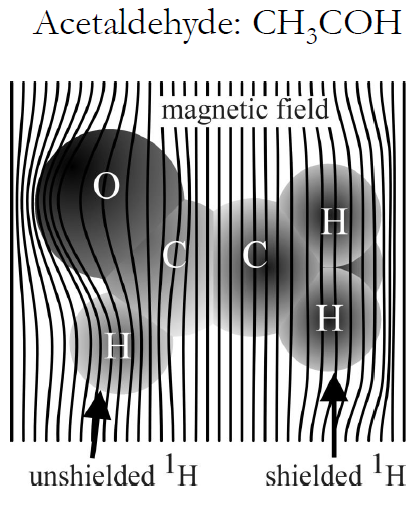
\includegraphics[scale=0.6]{acetaldeide.png}\quad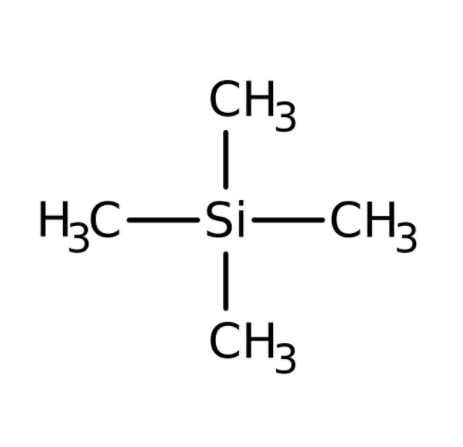
\includegraphics[scale=0.687]{tms.png}
\caption{\label{fig:tms} \textit{A sinistra, azione deformante dell'acetaldeide, e in particolare dell'ossigeno, sul campo magnetico; a destra, struttura del tetrametilsilano}.}
\end{figure}

\subsection{Interazione scalare}
L'\textbf{interazione scalare} è un'interazione indiretta tra gli spin nucleari, mediata dalle nuvole elettroniche degli orbitali molecolari. In breve, lo spin di un nucleo interagisce con la sua nuvola elettronica, polarizzandola, e quest'ultima trasmetterà la perturbazione ai nuclei appartenenti allo stesso orbitale molecolare del primo nucleo. È, dunque, un'interazione che coinvolge solo atomi direttamente legati in una molecola. L'hamiltoniana che descrive l'energia dell'interazione scalare dipende dagli spin dei due nuclei accoppiati e da uno scalare \textit{J}, che per il protone assume un valore compreso fra 0 e 18\,Hz e a sua volta dipende dagli angoli di legame fra il nucleo che ci interessa e quello a cui è direttamente legato. Di conseguenza, l'interazione scalare non dipenderà dal campo magnetico esterno applicato alla molecola ma solo dalla struttura di quest'ultima; quindi, a differenza dello spostamento chimico, non sarà necessario creare una scala assoluta per poter esprimere coerentemente il dato. L'equazione della magnetizzazione che tiene conto dell'interazione scalare è:
\begin{equation}
    S(t) = S_0\,\mathrm{e}^{\mathrm{i}(\omega_0t + \varphi)}\mathrm{e}^{\mathrm{i} \uppi Jt}\mathrm{e}^{-\frac{t}{\mathrm{T_2}}} \,,
    \label{3.6.3}
\end{equation}
dove $\varphi$ è l'angolo diedro caratteristico del legame fra i nuclei, $\omega_0$ è la pulsazione di Larmor e $\mathrm{T_2}$ è il tempo di rilassamento trasversale. Concentrandoci sull'andamento temporale del segnale, si deduce che si ha il massimo quando $t = \dfrac{1}{2J}$, perciò bisogna scegliere il tempo di eco $T_\mathrm{E}$ sulla base del valore di \textit{J}.

\begin{wrapfigure}{R}{0.495\textwidth}
    \centering
    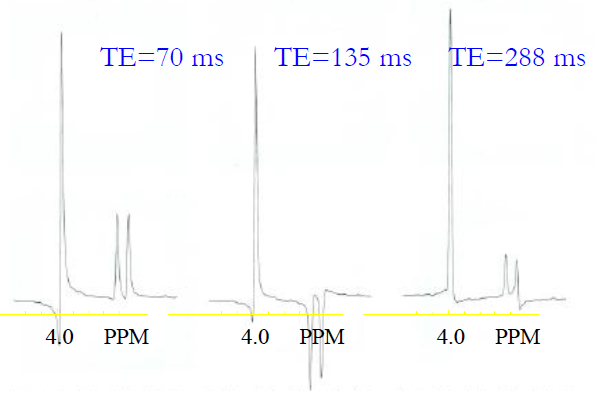
\includegraphics[width=0.495\textwidth]{al.png}
    \caption{\textit{Spettro NMR dell'acido lattico}.}
    \label{fig:al}
\end{wrapfigure}

Nella \figref{fig:al} è raffigurato lo spettro NMR dell'acido lattico, una molecola che viene prodotta da alcuni tipi di cellule tumorali che si sviluppano nel cervello. Si può notare che, scegliendo tempi di eco sempre maggiori, il segnale cambia d'intensità, passando da positivo a negativo e poi di nuovo positivo, indicando quindi un andamento \virgolette{periodico}, come ci si aspetta dall'\eqref{3.6.3}. Ciò può essere utile se il segnale non è di per sé molto intenso, per poter distinguere meglio il segnale proveniente dalle singole molecole in uno spettro che ne comprende diverse; fare in modo che alcuni di questi segnali siano ribaltati potrebbe rendere la figura più chiara. In realtà, l'andamento non è realmente periodico, perché si vede che l'ampiezza del segnale nella terza immagine è minore dell'ampiezza del segnale della prima, a causa del termine dovuto al rilassamento trasversale. Infine, osserviamo che i picchi sulla destra dello spettro dovrebbero essere un unico picco: anche questo è un effetto dell'interazione scalare. Il fenomeno della separazione dei picchi è complesso e trova spiegazione nella meccanica quantistica, ma è possibile individuare una semplice regola, illustrata nella \figref{fig:picchi}, per prevedere la distanza che separa i picchi, la loro intensità e il loro numero. Partendo dalla distanza fra i picchi, questa è costante ed è pari a \textit{J} della molecola, quindi dell'ordine degli hertz. Il numero di picchi osservati è $n+1$, dove \textit{n} è il numero di nuclei vicini con lo stesso spin presenti nella molecola. Infine, il rapporto fra le intensità dei picchi è fornito dal triangolo di Tartaglia.

L'importanza dello spostamento chimico e dell'interazione scalare per la MRS sta nel fatto che essi permettono di acquisire informazioni molto dettagliate sulle molecole presenti nei tessuti degli organismi, cosa che non è affatto scontata, vista la complessità delle molecole che si possono incontrare.

\begin{figure}[htp]
\centering
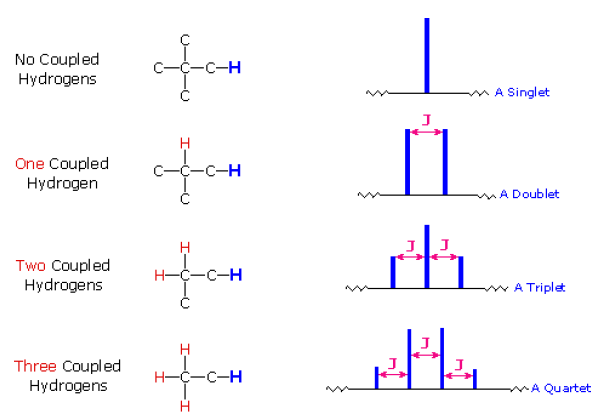
\includegraphics[scale=0.75]{picchi.png}\quad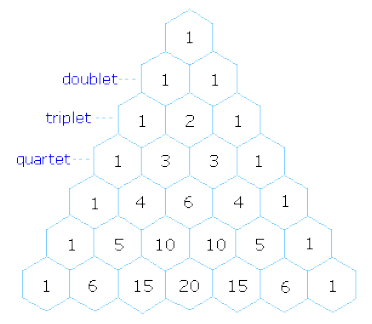
\includegraphics[scale=0.8]{tartaglia.png}
\caption{\label{fig:picchi} \textit{A sinistra, la regola \virgolette{$n+1$}; a destra, il triangolo di Tartaglia}.}
\end{figure}

\subsection{Sequenze per MRS}
Le due principali sequenze utilizzate in spettroscopia di risonanza magnetica sono la STEAM e la PRESS.

La \underline{STEAM} (\textit{stimulated echo acquisition mode}) è costituita da tre impulsi di 90°, come mostrato nella \figref{fig:steam}: 
\begin{itemize}[label=$-$]
    \item se la magnetizzazione inizialmente è orientata lungo l'asse \textit{z}, il primo impulso la porterà sul piano \textit{xy}, e per tutto il periodo $\frac{T_\mathrm{E}}{2}$ viene attivato il gradiente di selezione lungo \textit{z};
    \item il secondo impulso orienterà la magnetizzazione lungo il semiasse \textit{-z} e contestualmente viene attivato il gradiente di campo magnetico lungo \textit{x};
    \item il terzo impulso porterà la magnetizzazione di nuovo sul piano \textit{xy} e contestualmente viene attivato il gradiente di campo magnetico lungo \textit{y}.
\end{itemize}
La STEAM ha diversi vantaggi: in primo luogo, il tempo di eco può essere reso molto breve, permettendo la rivelazione dei nuclei caratterizzati da valori di $\mathrm{T_2}$ piccoli. Inoltre, gli impulsi di 90° consentono di ottenere voxel con bordi molto ben definiti e di limitare la radiazione trasferita alla materia d'indagine.

La \underline{PRESS} (\textit{point-resolved spectroscopy}) è costituita da un impulso di 90° e due impulsi di 180°, come mostrato nella \figref{fig:press2}, e il processo è simile a quanto fatto per la STEAM. La PRESS è caratterizzata da un buon rapporto segnale/rumore, ma per ottenere voxel con bordi ben definiti è necessario impiegare dei gradienti di campo magnetico efficienti (maggiori di 22\,mT/m). Il principale svantaggio della PRESS sono i tempi di eco inevitabilmente lunghi, con i quali non si riescono a rivelare i nuclei caratterizzati da valori di $\mathrm{T_2}$ piccoli: ciò la rende inutilizzabile, ad esempio, per la rivelazione del $\mathrm{^{31}P}$. Inoltre, questo influisce anche sulla radiazione trasmessa al campione indagato, che è maggiore. Nella \figref{fig:press2} è anche mostrato il procedimento di selezione fino al voxel finale: con il primo impulso si seleziona una sezione del campione, con il secondo si seleziona un parallelepipedo molto stretto e con il terzo il voxel finale.

\begin{figure}[htp]
\centering
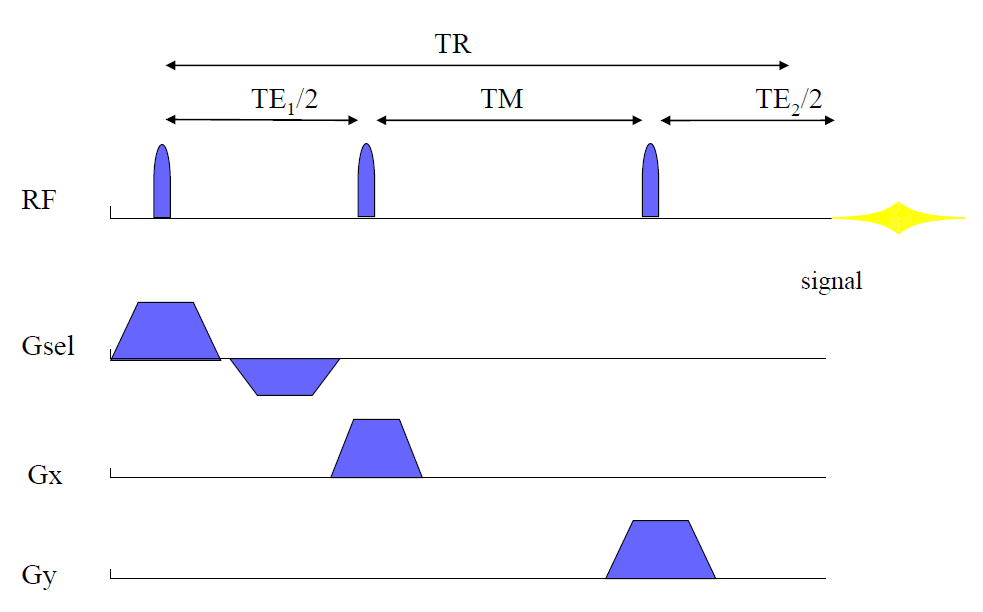
\includegraphics[scale=0.55]{steam.png}
\caption{\label{fig:steam} \textit{Sequenza STEAM}.}
\end{figure}

\begin{figure}[htp]
\centering
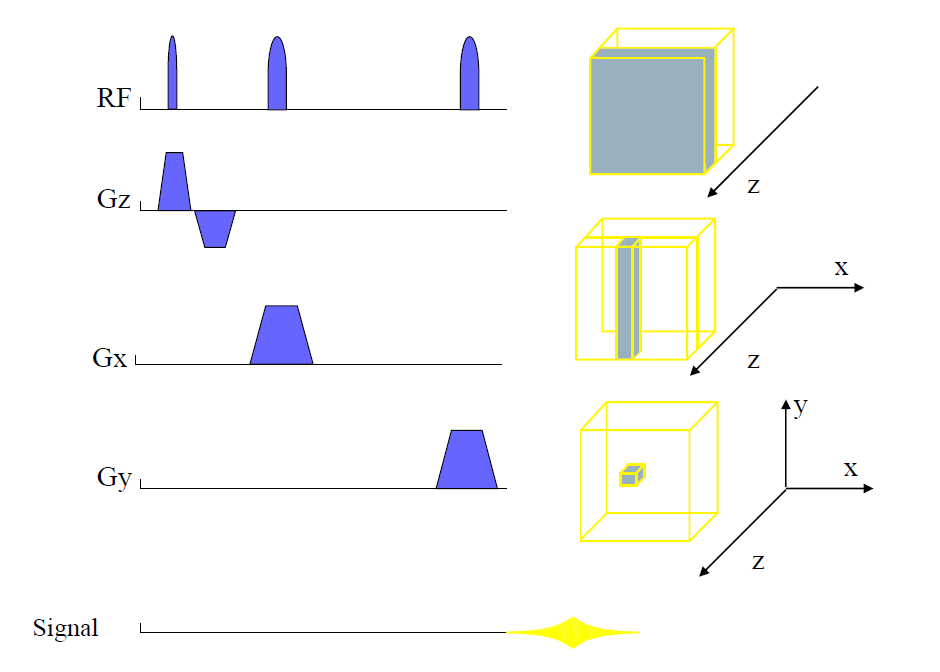
\includegraphics[scale=0.6]{press2.png}
\caption{\label{fig:press2} \textit{Sequenza PRESS con rappresentazione delle sezioni selezionate passaggio per passaggio}.}
\end{figure}

\begin{figure}[htp]
\centering
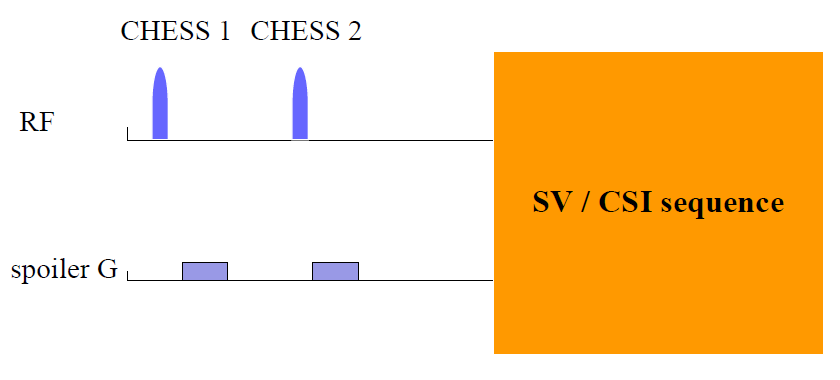
\includegraphics[scale=0.6]{chess.png}
\caption{\label{fig:chess} \textit{Metodo di soppressione CHESS}.}
\end{figure}

Bisogna, adesso, porsi il problema della soppressione dei segnali che non ci interessa acquisire e che provengono dal campione che analizziamo. Un caso importante è la soppressione del segnale proveniente dall'acqua, che in alcune zone del cervello, per fare un esempio, è di diversi ordini di grandezza più abbondante di metaboliti che di solito è interessante rivelare, come la creatina, la colina e l'N-acetilaspartato; di conseguenza, in una MRS di protone il segnale proveniente dagli $\mathrm{^1H}$ coprirebbe di gran lunga tutti gli altri segnali. Il metodo più usato per la soppressione di segnale coprente indesiderato è il metodo CHESS.

Il \underline{CHESS} (\textit{chemical shift selective pulses}) consiste di due passaggi, illustrati nella \figref{fig:chess}. Per prima cosa si ha l'applicazione di uno o più impulsi selettivi di tipo $\senc{x}$, con frequenza pari alla frequenza di Larmor dei nuclei della molecola di cui si vuole sopprimere il segnale. L'impulso selettivo porta la magnetizzazione di quella sola molecola dall'asse \textit{z} al piano \textit{xy}. Il secondo passaggio consiste, invece, nell'applicazione di un forte gradiente, che provoca lo sfasamento degli spin e la scomparsa della magnetizzazione da sopprimere. Se le molecole di cui si vuole sopprimere il segnale sono di diverso tipo (ad esempio acqua e grassi), basta applicare in sequenza due impulsi alle opportune frequenze e due gradienti. 

Dopo aver selezionato il singolo voxel con una sequenza STEAM o PRESS e aver soppresso il segnale che non è utile all'indagine, bisogna occuparsi dei metodi che consentono di mappare il volume del campione: i due metodi principali sono la SV e la sua evoluzione, la CSI.

Il metodo \underline{\textit{single voxel}} (SV-MRS) prevede il campionamento di un piccolo volume nella regione di interesse. Questa tecnica è caratterizzata da un buon rapporto segnale/rumore, tempi di esecuzione rapidi e una buona risoluzione spaziale, ma permette di studiare solo una piccola regione.

Il metodo \underline{\textit{chemical shift imaging}} (CSI-MRS), invece, prevede il campionamento di più voxel, ossia di una regione più grande. Ciò però la rende una tecnica caratterizzata da un rapporto segnale/rumore più basso e da tempi di esecuzione molto più lunghi rispetto alla SV. Il funzionamento della CSI è fondamentalmente analogo a quello della SV, ma ripetuto per quanti sono i voxel che si vogliono acquisire. Se immaginiamo di aver acquisito un voxel all'interno dell'area dello scanner e vogliamo acquisirne un altro adiacente, bisogna semplicemente modificare uno dei gradienti $G_x$ o $G_y$, in base alla direzione lungo la quale ci si vuole spostare rispetto al primo voxel acquisito per selezionare il secondo (si veda la \figref{fig:csi2d}). Se si vuole condurre un'indagine 2D, basta semplicemente continuare a modificare i due gradienti fino a quando non è stata acquisita tutta la sezione. Se, invece, si vuole estendere l'indagine a più sezioni, fino anche a tutto il volume del campione posto all'interno dello scanner, bisogna modificare il gradiente di selezione lungo \textit{z}, facendo riferimento alla \figref{fig:csi3d}. Il tempo di acquisizione totale per una 2D-CSI sarà dato da $N_x \times N_y \times T_\mathrm{R}$, mentre per una 3D-CSI sarà $N_x \times N_y \times N_z \times T_\mathrm{R}$, dove $N_i$ è il numero di voxel lungo la generica direzione \textit{i} e $T_\mathrm{R}$ è il tempo di ripetizione. I tempi di acquisizione, come si può intuire, possono arrivare a essere parecchio lunghi e questo può portare a una diminuzione eccessiva del rapporto segnale/rumore. Una \virgolette{soluzione} è quella di aumentare il volume dei voxel, in modo da mappare lo stesso volume in meno tempo, ma ciò influisce negativamente sulla risoluzione spaziale: insomma, nella pratica bisogna sempre trovare un compromesso per ottenere dei risultati adatti alla situazione.

\begin{figure}[htp]
\centering
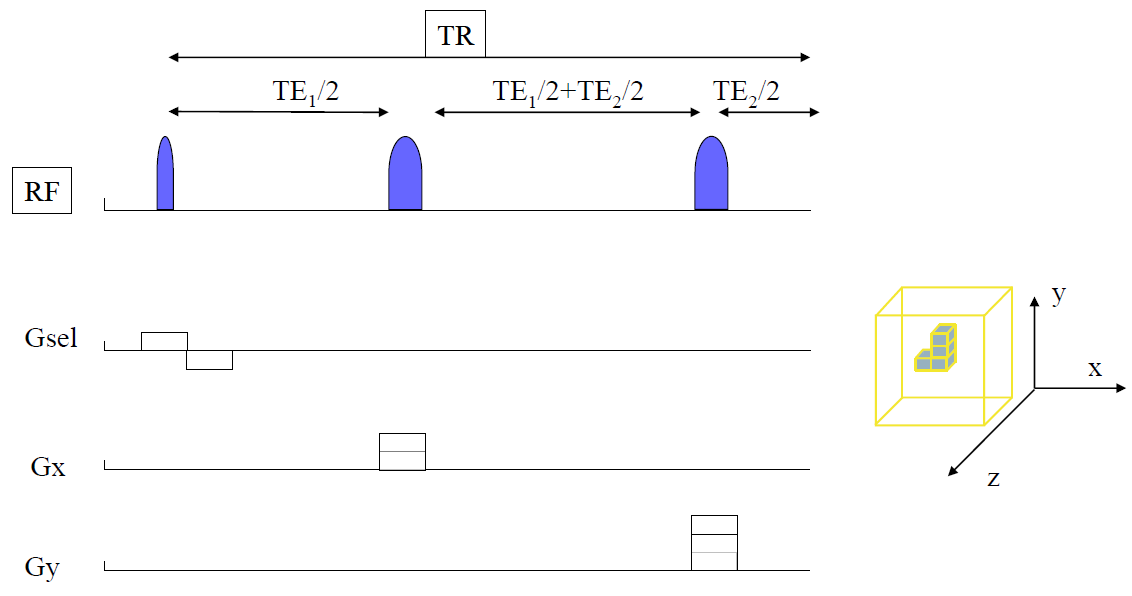
\includegraphics[scale=0.57]{csi2d.png}
\caption{\label{fig:csi2d} \textit{Sequenza PRESS 2D-CSI}.}
\end{figure}

\begin{figure}[htp]
\centering
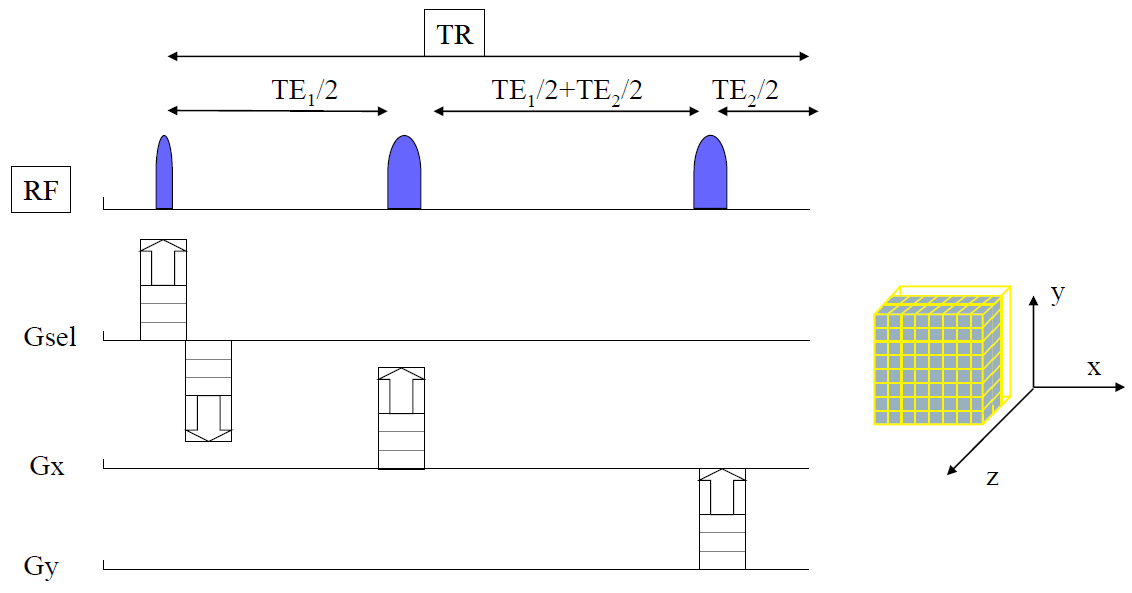
\includegraphics[scale=0.6]{csi3d.png}
\caption{\label{fig:csi3d} \textit{Sequenza PRESS 3D-CSI}.}
\end{figure}

\subsection{Acquisizione MRS}
L'acquisizione per la spettroscopia di risonanza magnetica avviene attraverso delle bobine, che possono sia trasmettere sia ricevere il segnale o solo riceverlo; in alcuni casi vengono usate in maniera combinata o, addirittura, possono essere introdotte all'interno del corpo per una migliore acquisizione.

Dopo che il paziente si è posizionato all'interno dello scanner, si esegue per prima cosa un'acquisizione veloce e poco risolta, chiamata \textit{scout image}, che serve solo a verificare che la posizione del paziente sia corretta; la \figref{fig:scout} è un esempio di \textit{scout image} in cui si vede chiaramente che il paziente deve ricollocarsi meglio all'interno dello scanner.

\begin{figure}[htp]
\centering
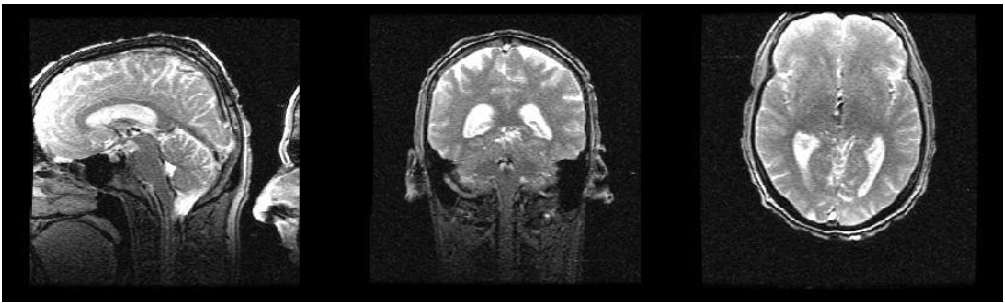
\includegraphics[scale=0.7]{scout.png}
\caption{\label{fig:scout} \textit{Scout image di un cervello}.}
\end{figure}

Il passo successivo è acquisire un'immagine generale e ben definita del volume di interesse, per avere una conoscenza generale della morfologia della regione da indagare; un esempio è fornito nella \figref{fig:gen}. A questo punto, bisogna rendere il campo magnetico $\Vec{B}_0$ il più omogeneo possibile, in modo da limitare gli effetti di spostamento chimico non dovuti agli atomi e alle molecole. Per verificare l'omogeneità del campo magnetico, si esegue una spettroscopia preliminare per acquisire il picco dei protoni nelle molecole d'acqua: se si osserva che l'ampiezza di tale picco è molto grande, significa che la disomogeneità del campo è grande e va migliorata. Infine, è necessario eliminare il segnale indesiderato con il metodo CHESS, applicando delle bande di saturazione come mostrato nella \figref{fig:bande}.

\begin{figure}[htp]
\centering
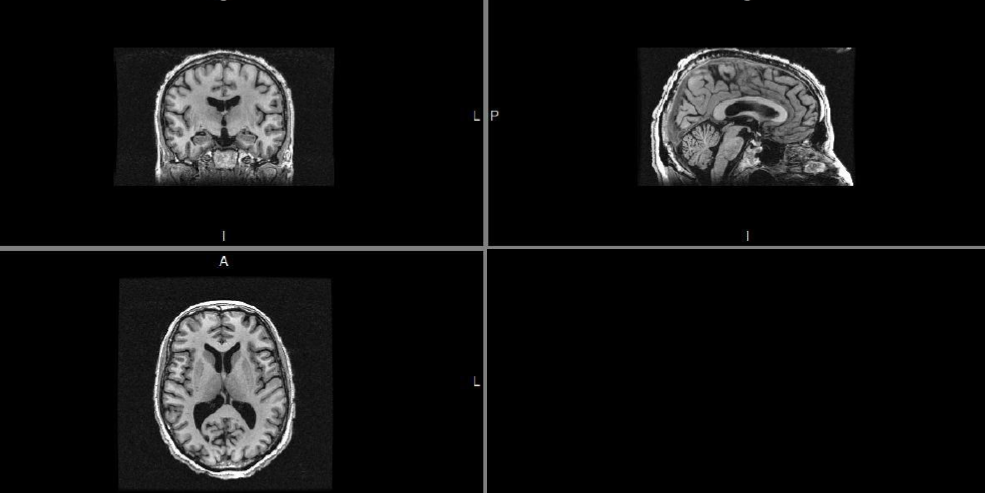
\includegraphics[scale=0.75]{gen.png}
\caption{\label{fig:gen} \textit{3D-MRI di un cervello}.}
\end{figure}

\begin{figure}[htp]
\centering
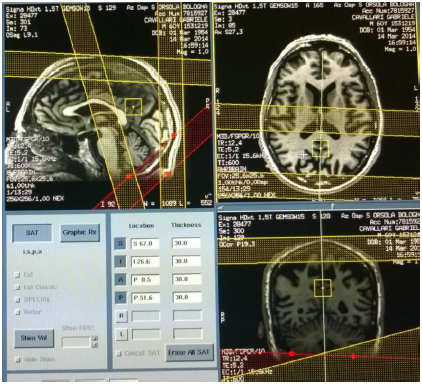
\includegraphics[scale=1.2]{bande.png}
\caption{\label{fig:bande} \textit{Bande di saturazione per la soppressione del segnale di acqua e grassi}.}
\end{figure}

\newpage

Per concludere, trattiamo brevemente il rapporto segnale/rumore (SNR). Più volte è già stato detto che aumentando il numero di acquisizioni di uno stesso segnale è possibile aumentare l'SNR. Il limite di questo approccio è il fatto che i tempi si allungano a dismisura, e la risonanza magnetica è una tecnica che già di per sé è caratterizzata da tempi lunghi. L'SNR dipende direttamente dal segnale \textit{S} e inversamente dal rumore \textit{N}. \textit{S} è proporzionale al numero di medie \textit{n}, poiché il segnale di ogni acquisizione si somma coerentemente con quelli di tutte le altre acquisizioni. \textit{N}, invece, segue una distribuzione casuale, poiché è dovuto al fatto che si lavora a temperatura ambiente e con componenti elettroniche che si riscaldano quando sono percorse da corrente; di conseguenza, \textit{N} è proporzionale alla radice di \textit{n}. Abbiamo quindi:
\begin{equation}
    \frac{S}{N} \propto \frac{n}{\sqrt{n}} = \sqrt{n}\,.
\end{equation}
Se ne deduce che, all'aumentare delle acquisizioni \textit{n}, l'SNR aumenta come $\sqrt n$.\\
Volendo fare un riepilogo, il rapporto segnale/rumore dipende dai seguenti fattori:
\begin{itemize}[label=$-$]
    \item nucleo, per via del rapporto giromagnetico $\gamma_\mathrm{n}$ che influisce sulla frequenza di Larmor;
    \item volume di interesse, per via del numero di metaboliti in esso presenti (più è grande, più ce ne saranno);
    \item concentrazione di metaboliti all'interno del volume di interesse, per lo stesso motivo del punto precedente;
    \item campo magnetico $\mathrm{B_0}$, poiché influisce sulla frequenza di Larmor;
    \item bobine impiegate, la cui sensibilità influisce sul campo magnetico $B_1$;
    \item numero di acquisizioni \textit{n};
    \item sequenza d'impulsi utilizzata.
\end{itemize}

\subsection{Post-elaborazione}
La post-elaborazione di un'acquisizione consiste di tutte le tecniche messe in atto ad acquisizione finita per evidenziare uno specifico segnale. In base alla situazione in cui ci si trova, è conveniente eseguire misurazioni di concentrazioni di metaboliti relative o assolute.

Una \underline{misurazione di concentrazione relativa} si occupa di misurare la concentrazione di un metabolita in una specifica regione in rapporto alla concentrazione di un altro metabolita. Nelle applicazioni cliniche, di solito, questa misurazione è sufficiente; nel caso del cervello, ad esempio, è usuale studiare la concentrazione relativa dell'N-acetilaspartato o della colina rispetto alla creatina. Tuttavia, nei casi di patologie in cui il metabolismo delle cellule è ridotto, potrebbe capitare di osservare una diminuzione di tutte e tre le molecole suddette in ugual misura: di conseguenza, una misurazione di concentrazione relativa darebbe gli stessi risultati per un tessuto sano e per uno malato.

Una \underline{misurazione di concentrazione assoluta}, invece, si può eseguire scegliendo un campione di riferimento che non sia uno dei metaboliti che possono subire riduzioni in caso di patologie. Il campione di riferimento può essere interno o esterno, ma è opportuno che sia interno, ovvero che il suo segnale e la sua concentrazione siano stati misurati nella stessa zona in cui si vuole misurare la concentrazione del metabolita che ci interessa. Di solito, l'acqua si rivela una buona scelta come campione di riferimento, perché restituisce un buon SNR e possiede un'alta concentrazione nei tessuti. Inoltre, se si parla del cervello, la concentrazione dell'acqua è piuttosto costante, variando leggermente per la materia bianca e per la materia grigia. Conoscere la concentrazione del campione di riferimento è fondamentale per poter calcolare la concentrazione del metabolita che ci interessa, in quanto:
\begin{equation}
    C_\mathrm{met} \propto C_\mathrm{acq} \frac{S_\mathrm{met}}{S_\mathrm{acq}}\,,
    \label{esterno}
\end{equation}
dove \textit{C} sono le concentrazioni e \textit{S} i segnali. Con un po' di attenzione ci si accorge, però, che l'\eqref{esterno} ha bisogno di alcune precisazioni. Infatti, secondo l'\eqref{segnale}, il segnale dipende dai tempi di rilassamento trasversale e longitudinale.

Per far sì che i segnali dell'acqua e del metabolita siano indipendenti da $\mathrm{T_2}$, è necessario acquisirli a  $T_\mathrm{E}$ molto minore di $\mathrm{T_2}$, idealmente nullo. Infatti, come mostrato nella \figref{fig:meta}, essi decadono in maniera diversa, a causa del fatto che il segnale dell'acqua non è un'esponenziale ma una somma di segnali esponenziali provenienti sia dall'interno sia dall'esterno delle cellule, quindi ogni altra scelta di $T_\mathrm{E}$ comprometterebbe l'acquisizione. Tuttavia, è impossibile ridurre il tempo di eco fino a renderlo nullo: l'unica soluzione è acquisire i due segnali per diversi tempi di eco e poi eseguire due fit separati, in modo da ottenere il valore del segnale a $T_\mathrm{E} = 0$ sia per l'acqua sia per il metabolita. Come spiegato in precedenza, se si acquisissero contemporaneamente i due segnali, quello dell'acqua coprirebbe completamente quello del metabolita, perciò sarà necessario eseguire due acquisizioni separate per le due sostanze; per l'acqua ci sarà bisogno di poche ripetizioni, poiché il segnale che restituisce è tipicamente intenso e di buona qualità, mentre per il metabolita, molto meno spazialmente concentrato dell'acqua, l'acquisizione dovrà essere ripetuta diverse volte. Rimossa la dipendenza da $\mathrm{T_2}$, rimane da eliminare la dipendenza da $\mathrm{T_1}$: per fare ciò, sempre secondo l'\eqref{segnale}, è sufficiente scegliere il tempo di ripetizione $T_\mathrm{R} \geq 5\mathrm{T_1}$ per entrambi i segnali. Dopo aver eseguito tutti i passaggi precedenti, il segnale acquisito dovrebbe essere grossomodo indipendente dai tempi di rilassamento, e l'\eqref{esterno} può essere migliorata:
\begin{equation}
    \boxed{C_\mathrm{met} = (0,75 \times 55,5 \times 10^3) \times \frac{S_{0,\mathrm{met}}}{S_{0,\mathrm{acq}}} \times \frac{n_\mathrm{a,acq}}{n_\mathrm{a,met}} \times \frac{n_\mathrm{H,acq}}{n_\mathrm{H,met}}}
\end{equation}
dove 0,75 è la densità dell'acqua, 55,5 è la molarità, $S_0$ sono i segnali indipendenti dai tempi di decadimento, $n_\mathrm{a}$ è il numero di acquisizioni di ciascun segnale e $n_\mathrm{H}$ è il numero di nuclei di idrogeno all'interno delle rispettive molecole.

\begin{figure}[htp]
\centering
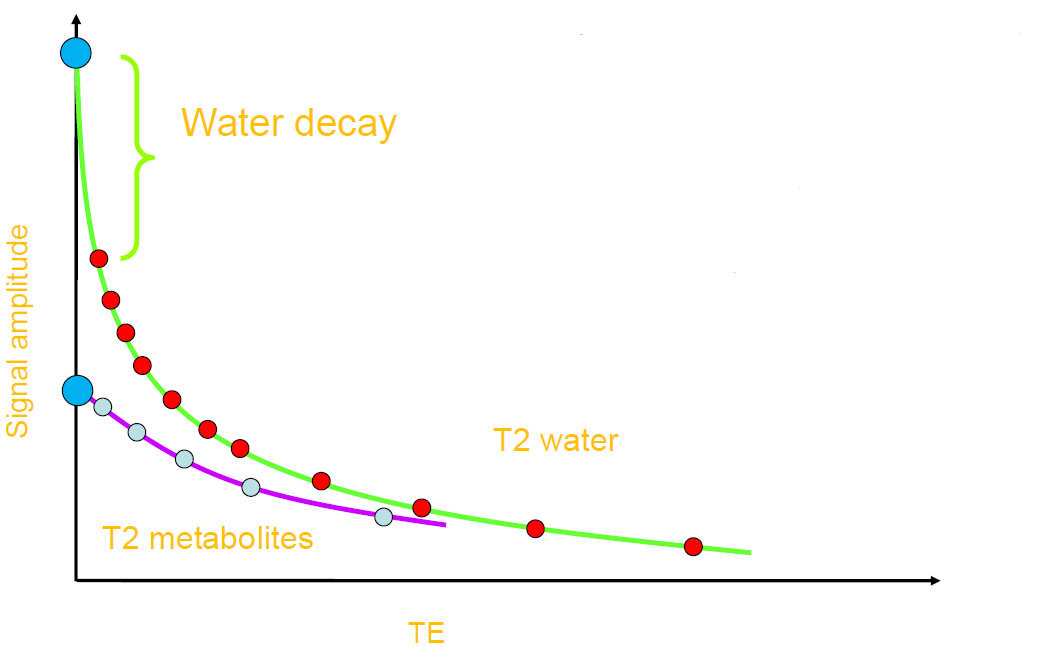
\includegraphics[scale=0.5]{meta.png}
\caption{\label{fig:meta} \textit{Grafico dei segnali di acqua e di un metabolita in funzione del tempo di eco}.}
\end{figure}

Le tecniche di post-elaborazione degli spettri per la quantificazione dell'ampiezza di ciascun segnale sono state principalmente tre. Inizialmente, fu scelta la tecnica di integrare ogni picco dello spettro, e quindi di calcolare l'area sottostante, ma questa tecnica funziona correttamente solo per spettri con pochi picchi. Successivamente, si pensò di eseguire sullo spettro un fit multigaussiano, ovvero eseguire un fit gaussiano separatamente per ogni picco dello spettro. Oggigiorno, invece, si utilizza una tecnica di fit con conoscenza a priori, cioè prima dell'acquisizione si effettua una simulazione delle molecole che ci si aspetta di trovare, o alternativamente si può preparare un campione artificiale con le molecole che ci si aspetta e si sottopone tale campione a spettroscopia. Poi si sovrappone lo spettro preliminare a quello ottenuto dall'indagine sulla materia da indagare, come mostrato nell'immagine di sinistra della \figref{fig:fit}: se il residuo della sovrapposizione è solo rumore, allora la previsione fatta è corretta e nello spettro si riuscirà a identificare il segnale di ciascun metabolita.

Nell'immagine di destra della \figref{fig:fit} sono riportati gli spettri dei più importanti metaboliti a livello neurologico. Si può notare come l'unico spettro veramente semplice sia quello della creatina, costituito da soli due picchi, mentre tutti gli altri presentano attività a diverse frequenze e spesso si sovrappongono. Se non si possiede una conoscenza preliminare dei metaboliti prima di fare l'acquisizione e il fit si rischia di perdere il segnale di una moltitudine di metaboliti.

\begin{figure}[htp]
\centering
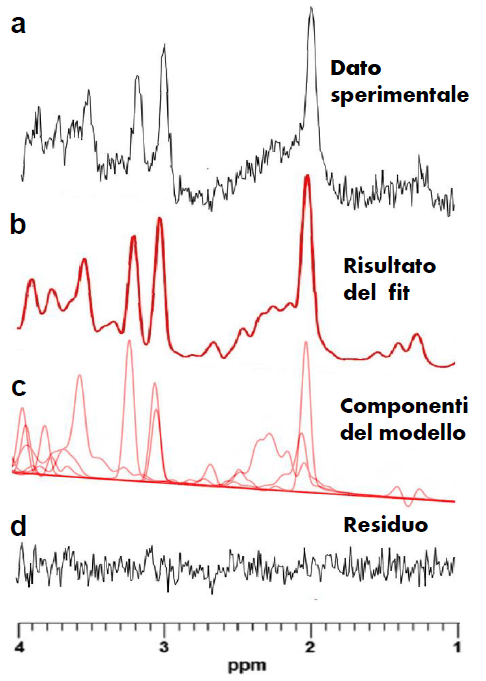
\includegraphics[scale=0.7]{fit.png}\quad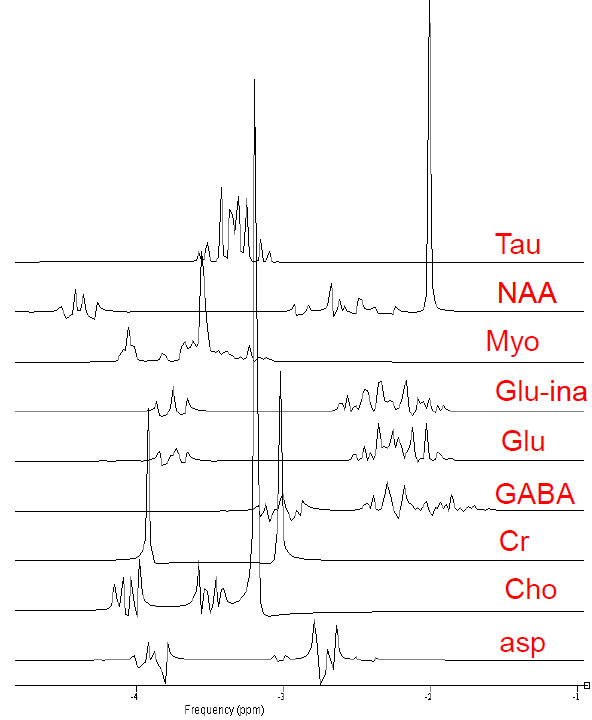
\includegraphics[scale=0.7]{meta2.png}
\caption{\label{fig:fit} \textit{A sinistra, fit multigaussiano con conoscenza preliminare; a destra, spettri dei principali metaboliti neurologici}.}
\end{figure}

\begin{figure}[htp]
\centering
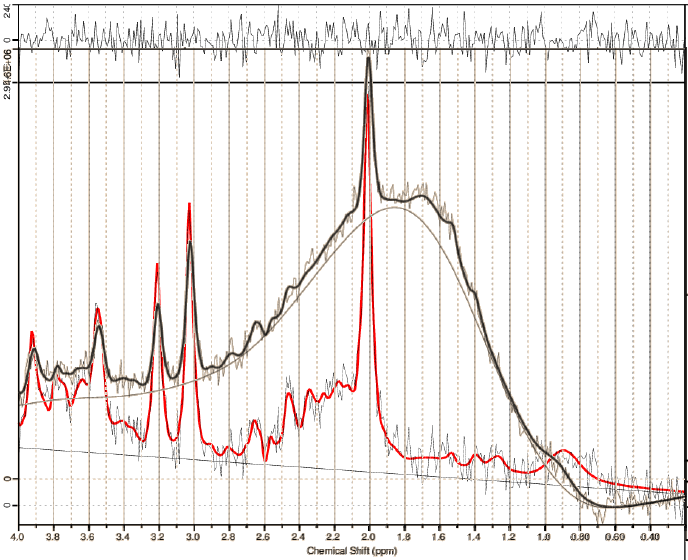
\includegraphics[scale=0.87]{gobba.png}
\caption{\label{fig:gobba} \textit{Spettro dovuto a contaminazione da lipidi (in nero) e spettro corretto (in rosso)}.}
\end{figure}

Per concludere, un ulteriore compito della post-elaborazione è quello di accorgersi di errori nell'acquisizione degli spettri. Nella \figref{fig:gobba} si possono osservare due spettri dello stesso volume di interesse, localizzato nel cervello: quello in nero presenta una gobba anomala dovuta a una non corretta soppressione del segnale proveniente dai lipidi, in questo caso presente nella cute. Risistemando meglio le bande di saturazione, si riesce a eliminare il segnale lipidico e a ottenere lo spettro corretto in rosso.
Nella \figref{fig:mov}, invece, si osserva uno sdoppiamento di ogni picco nella immagine a), chiaro segno che il paziente si è mosso durante l'acquisizione, di conseguenza le frequenze di emissione che prima erano associate a una certa posizione nello spazio, dopo il movimento saranno associate a una nuova posizione, e la macchina registrerà due frequenze per lo stesso metabolita.

\begin{figure}[htp]
\centering
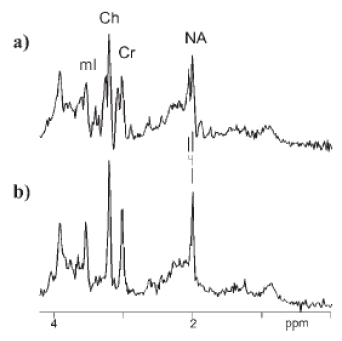
\includegraphics[scale=1]{mov.png}
\caption{\label{fig:mov} \textit{Spettri di metaboliti neurologici, di cui a) è stato acquisito in maniera scorretta per un movimento del paziente}.}
\end{figure}

\subsection{Applicazioni}
Nella \figref{fig:spettro} è raffigurato lo spettro di protone dei principali metaboliti neurologici.

L'N-acetilaspartato (NAA) è una molecola presente solo in neuroni e dendriti e rappresenta uno dei marker più importanti per il sistema nervoso. Il suo picco principale si trova circa a 2\,ppm ed è dovuto ai tre nuclei di idrogeno del gruppo metilico presente nella molecola, mentre il segnale degli altri nuclei di idrogeno cade nelle frequenze dei Glx, tra i 2 e i 3\,ppm.\\
Le molecole che rientrano nel gruppo Glx sono glutammato (Glu), glutammina (Gln) e GABA. Svolgono un importante ruolo nella neurotrasmissione e le loro molecole sono molto simili, differendo di poco anche dall'NAA, ragion per cui i loro spettri condividono le stesse frequenze. I Glx non si riescono a distinguere chiaramente con un campo applicato di 1,5\,T, perché l'SNR sarebbe troppo alto.\\
La creatina e la fosfocreatina, indicate con la sigla tCr, sono dei marker per il metabolismo energetico perché agiscono come riserve di gruppi fosfato dai quali viene prodotto ATP. Il picco principale delle tCr si trova a circa 3 ppm ed è dovuto, come per l'NAA, ai tre nuclei di idrogeno del gruppo metilico, mentre il segnale dei nuclei presenti nel gruppo $\mathrm{-CH_2}$ viene emesso a 3,9\,ppm.\\
La colina, la fosfocolina e la glicerofosforilcolina (tCho) sono associate al metabolismo della membrana cellulare. Il picco principale delle tCho si trova a 3,2\,ppm ed è dovuto ai nuclei di idrogeno dei tre gruppi metilici legati all'azoto. Gli spettri delle singole molecole del gruppo sono visibili solo a campi magnetici molto alti.\\
Il mio-inositolo (mI) è un marker dell'accrescimento cellulare e il suo picco, emesso indistintamente dai nuclei di idrogeno non legati all'ossigeno, si trova a 3,6\,ppm.\\
Gli spettri dell'acido lattico (Lac) e dei lipidi (Lip) sono dovuti entrambi ai nuclei di idrogeno presenti nei gruppi metilici e non sono visibili con campi applicati di 1,5\,T, poiché verrebbero coperti dal rumore. La produzione di acido lattico è associata ad alcuni tipi di tumore, mentre lo spettro dei lipidi può essere dovuto a una non perfetta soppressione del segnale oppure ad alcune patologie.

\begin{figure}[htp]
\centering
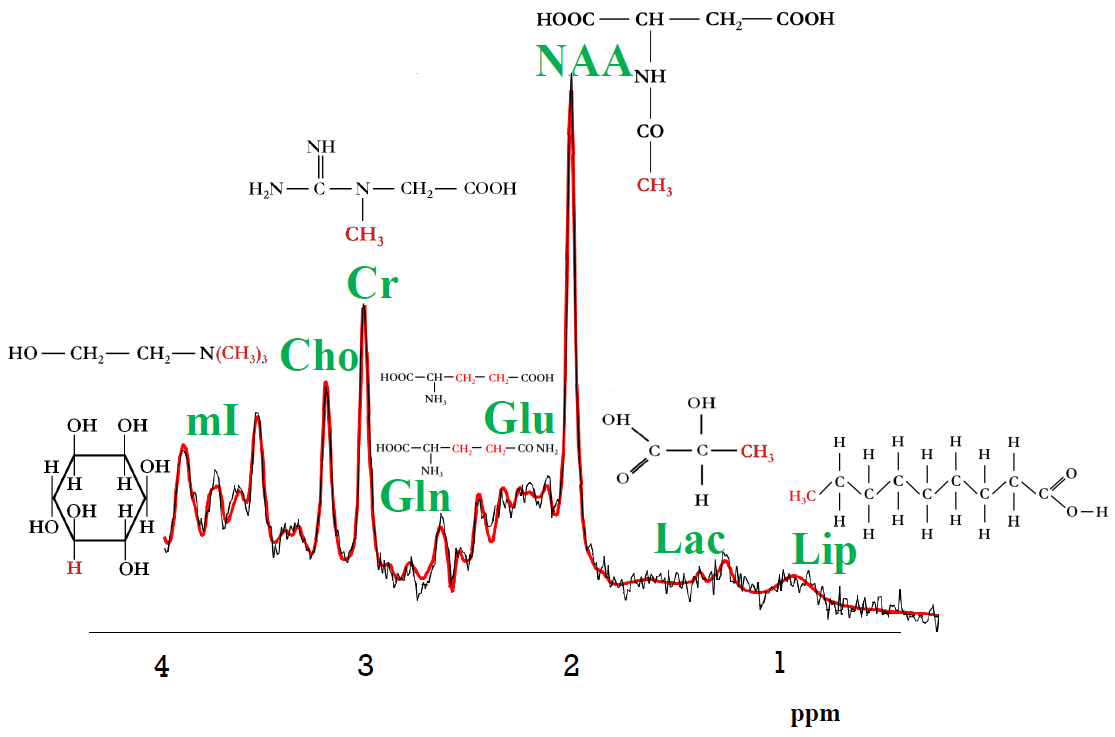
\includegraphics[scale=0.63]{spettro.png}
\caption{\label{fig:spettro} \textit{Spettri di metaboliti neurologici}.}
\end{figure}

\begin{figure}[htp]
\centering
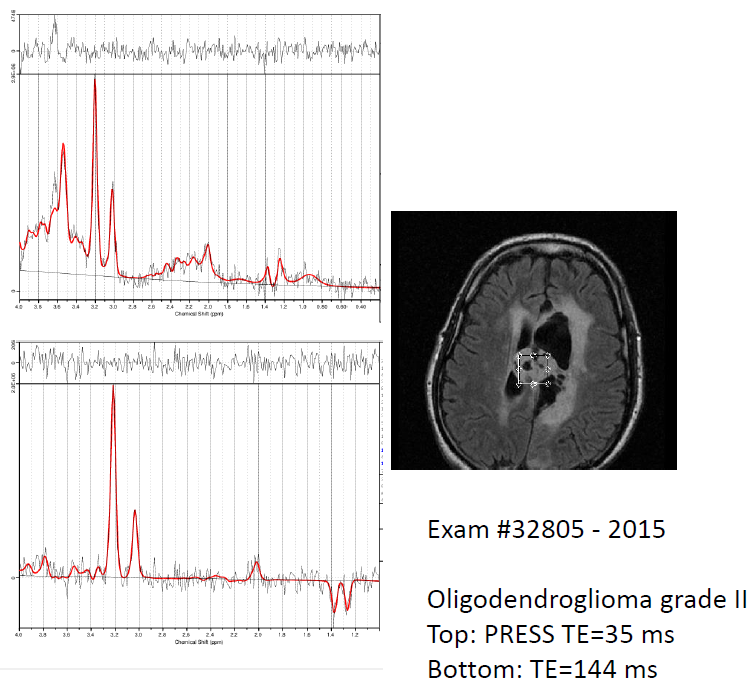
\includegraphics[scale=0.8]{tum.png}
\caption{\label{fig:tum} \textit{Spettroscopie con diversi tempi di eco, alterate da un tumore cerebrale}.}
\end{figure}

Nella \figref{fig:tum} si possono osservare due spettroscopie eseguite a tempi di eco diversi che possono essere associate a un tumore del tessuto connettivo cerebrale. Le cose che saltano più all'occhio guardando lo spettro sono la scomparsa quasi totale degli spettri di NAA, Glx e mI, l'ultimo perché caratterizzato da un $\mathrm{T_2}$ piccolo. Al contrario, si ha un'intensità molto grande per il segnale della colina, proprio perché quel tipo di tumore è soggetto a un accrescimento massiccio, di conseguenza il metabolismo della membrana cellulare è aumentato. In più, è presente anche acido lattico, visibile soprattutto nell'immagine inferiore in antifase.

Per studiare le patologie con questa metodica è necessario conoscere anche gli spettri dei singoli metaboliti in gruppi di controllo composti da individui sani, e bisogna anche dividere i gruppi di controllo in base a differenze regionali e anagrafiche. Nella \figref{fig:controllo} è riportato uno studio effettuato su soggetti sani fra i 50 e i 90 anni, per monitorare l'andamento di alcuni metaboliti nella materia bianca del cervello. Come si può notare, non c'è nessuna correlazione tra l'invecchiamento e la presenza di NAA, Cho e mI, mentre è stato rilevato un aumento significativo della creatina con l'età.

\begin{figure}[htp]
\centering
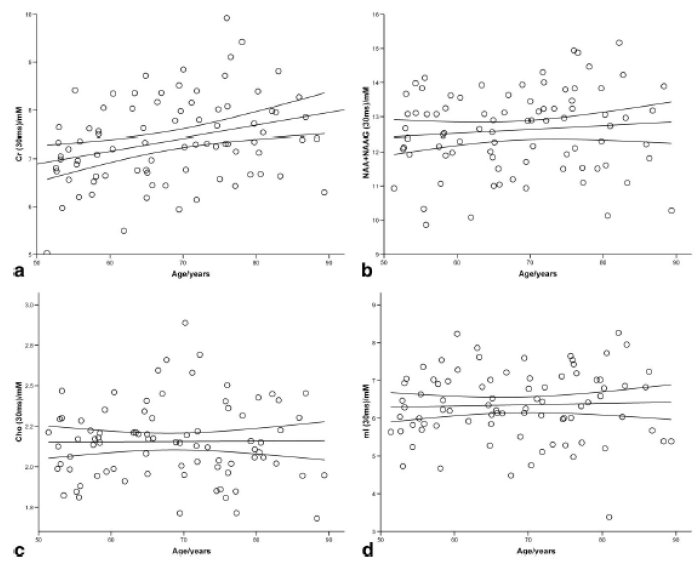
\includegraphics[scale=0.72]{controllo.png}
\caption{\label{fig:controllo} \textit{Andamento di Cr, NAA, Cho e mI in gruppi di controllo sani in funzione dell'età}.}
\end{figure}

\begin{figure}[htp]
\centering
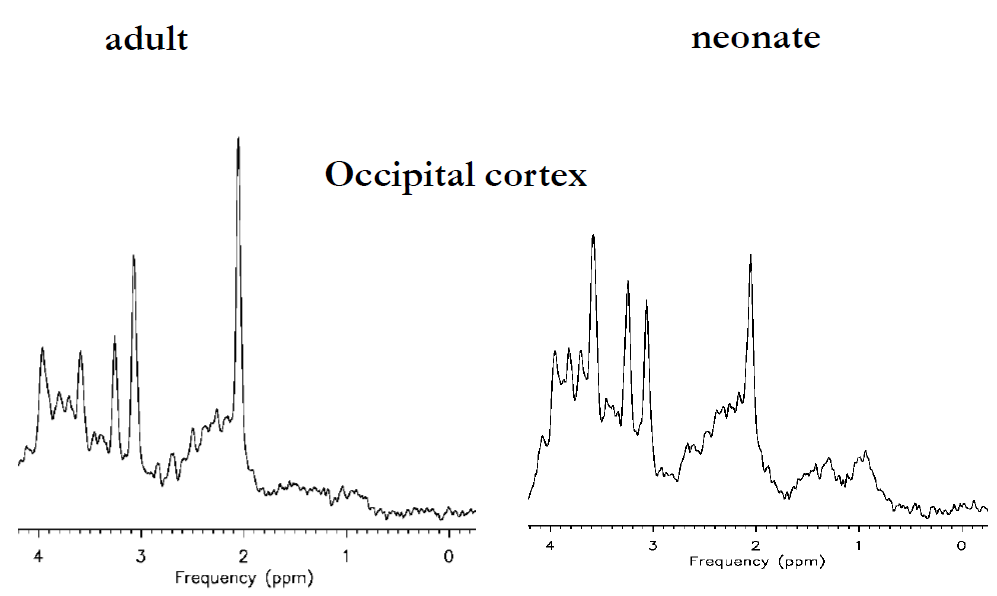
\includegraphics[scale=0.55]{controllo2.png}
\caption{\label{fig:controllo2} \textit{Spettroscopia della corteccia occipitale in un adulto e in un neonato sani}.}
\end{figure}

Nella \figref{fig:controllo2} si osserva, invece, come la variazione, anche significativa, della concentrazione di metaboliti cerebrali in individui sani non sia esclusivamente correlata a una patologia. Infatti, nella spettroscopia effettuata sul neonato si vedono dei livelli molto alti di Cho e mI, ma questi possono essere semplicemente associati al veloce accrescimento dei tessuti nei bambini.\\
La concentrazione dei metaboliti può subire variazioni anche considerando zone diverse del cervello. Ad esempio, tipicamente sia la creatina sia i Glx sono più concentrati nella materia grigia che non nella bianca, mentre l'N-acetilaspartato rimane piuttosto costante.

Nel 2013, sono stati definiti gli ambiti di applicazione in cui la MRS ha più ragione di essere impiegata:
\begin{itemize}[label=$-$]
    \item tumori cerebrali;
    \item lesioni infettive focali;
    \item disordini metabolici;
    \item asfissia perinatale;
    \item sclerosi multipla;
    \item disordini di demielinizzazione;
    \item demenze;
    \item epilessia focale;
    \item sclerosi mesiale temporale;
    \item lesioni ischemiche.
\end{itemize}
In particolare nell'ambito dei tumori cerebrali, l'MRS è complementare all'MRI nei casi di:
\begin{itemize}[label=$-$]
    \item diagnosi istologica;
    \item stadiazione tumorale;
    \item guida per biopsia intracraniale;
    \item prognosi;
    \item pianificazione per trattamenti chirurgici e non;
    \item diagnosi differenziale per tumori recidivanti e lesioni post-terapiche.
\end{itemize}

\begin{figure}[htp]
\centering
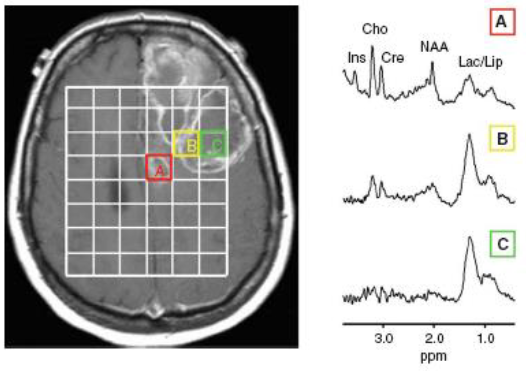
\includegraphics[scale=0.85]{glio.png}
\caption{\label{fig:glio} \textit{Imaging e spettroscopia di un cervello affetto da glioblastoma}.}
\end{figure}

\noindent Vediamo alcuni esempi di tumori in cui la spettroscopia e l'\textit{imaging} vengono utilizzati insieme.

Nella \figref{fig:glio} è riportata un'immagine diagnostica in cui si riconosce un glioblastoma, un tumore che colpisce il tessuto connettivo cerebrale, accompagnato da spettroscopia per tre voxel particolari. Nel voxel A, come ci si potrebbe aspettare, si osserva una diminuzione di NAA e creatina e un incremento di colina, acido lattico e lipidi, il quale, se la soppressione del segnale del tessuto adiposo cutaneo è stata eseguita correttamente, non dovrebbe apparire. Nei voxel B e C, invece, si osserva una quasi completa scomparsa di tutti i metaboliti, a eccezione dell'acido lattico e dei lipidi, il che indica perdita di funzionalità del tessuto, morte cellulare e accelerato metabolismo delle membrane cellulari dovuto alla crescita del tessuto canceroso.

Nella \figref{fig:astro} si osserva un altro tipo di tumore, l'astrocitoma, e anche qui si osserva una concentrazione ridotta di NAA, un aumento di Cho, ma stavolta non è presente segnale proveniente dai lipidi.

\begin{figure}[htp]
\centering
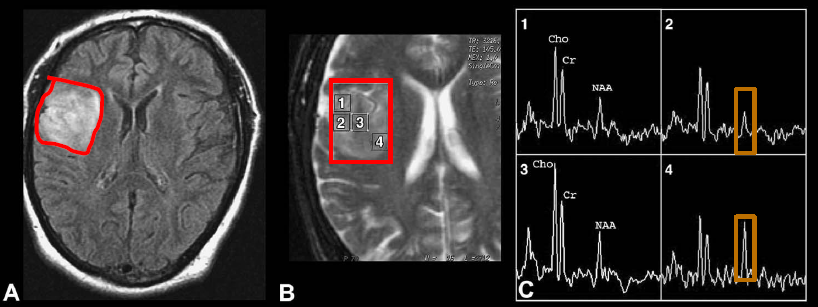
\includegraphics[scale=0.86]{astro.png}
\caption{\label{fig:astro} \textit{Immagini pesate in $\mathrm{T_2}$ con metodi diversi e spettroscopia di un cervello affetto da astrocitoma}.}
\end{figure}

\begin{figure}[htp]
\centering
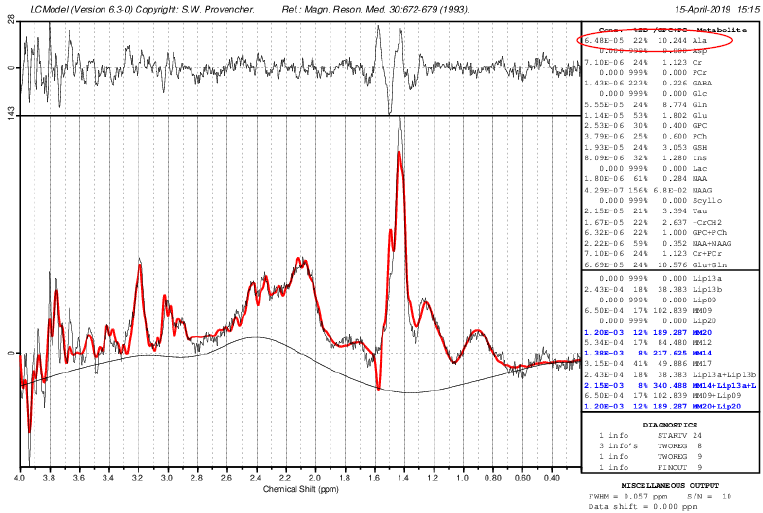
\includegraphics[scale=0.96]{meni.png}
\caption{\label{fig:meni} \textit{Spettroscopia di un voxel di tessuto affetto da meningioma}.}
\end{figure}

Nella \figref{fig:meni} è raffigurato il risultato della spettroscopia di un tessuto affetto da meningioma. Si osserva come il segnale della colina sia aumentato mentre quello dell'N-acetilaspartato, che si confonde con i Glx, sia ridotto. Sebbene possa sembrare diversamente, il picco fra 1,4 e 1,5\,ppm non è quello dell'acido lattico ma di un amminoacido, l'alanina (Ala), che è condizione non necessaria ma sufficiente per poter capire che ciò che si sta osservando è un meningioma. In generale:
\begin{itemize}[label=$-$]
    \item per tumori di basso grado si osserva un aumento di Cho e mI e una diminuzione di NAA e Cr;
    \item per tumori di alto grado si osserva un aumento di Cho, Lip e Lac e una diminuzione di NAA e Cr;
    \item in caso di metastasi si ha lo stesso spettro dei tumori di alto grado ma con sparizione completa dell'NAA;
    \item in caso di meningioma, si osserva un aumento di Cho e Ala e una diminuzione di NAA e Cr.
\end{itemize}

Non tutte le alterazioni degli spettri sono indice di tumori. Nella \figref{fig:ks} è mostrato il risultato di una spettroscopia eseguita sul cervello di un paziente affetto da sindrome di Kearns-Sayre, che indica una concentrazione aumentata di colina e acido lattico, sebbene il tessuto non presenti alcuna lesione. Un esempio \virgolette{opposto} in un certo senso, che comporta un forte aumento di concentrazione di NAA e mI e una lieve diminuzione di Cho, è quello della sindrome di Canavan, una malattia che si manifesta già in età neonatale a causa della mutazione di un gene che codifica l'enzima aspartoacilasi, responsabile dell'eliminazione dell'N-acetilaspartato. Nella \figref{fig:canavan} sono riportati due spettri, riguardanti un soggetto sano e uno malato.

\begin{figure}[htp]
\centering
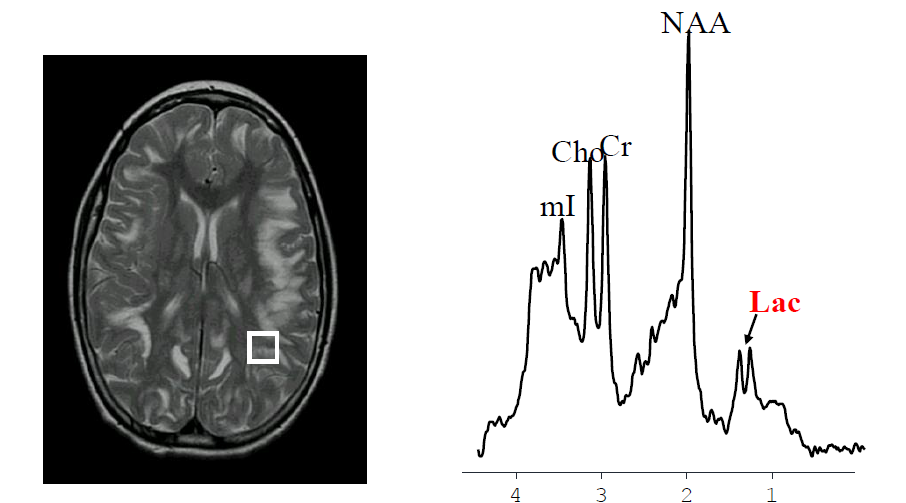
\includegraphics[scale=0.57]{ks.png}
\caption{\label{fig:ks} \textit{Spettroscopia di un voxel di cervello affetto da sindrome di Kearns-Sayre}.}
\end{figure}

\vspace{-10 pt}

\begin{figure}[htp]
\centering
\includegraphics[scale=0.78]{canavan.png}
\caption{\label{fig:canavan} \textit{Spettroscopie sul cervello di un neonato sano e di uno affetto da sindrome di Canavan}.}
\end{figure}

\noindent Un ultimo esempio è costituito dall'encefalopatia ipossico-ischemica perinatale (EII), che si manifesta sotto forma di lesioni nel cervello del neonato a causa di una carenza di ossigeno durante il parto. Di solito per la diagnosi è sufficiente un elettroencefalogramma o altri esami clinici; tuttavia, a volte è necessario sottoporre il neonato a MRS, di cui un esempio è riportato nella \figref{fig:asfissia}, dove si possono notare una diminuzione di NAA e un aumento di lipidi e acido lattico; la variazione è tanto maggiore quanto più grave è stata l'ischemia.

\begin{figure}[htp]
\centering
\includegraphics[scale=0.7]{asfissia.png}
\caption{\label{fig:asfissia} \textit{Spettroscopie sul cervello di un neonato sano e di uno affetto da EII}.}
\end{figure}

\section{Tecniche di MRI}
Dopo aver visto le basi del funzionamento dell'\textit{imaging} di risonanza magnetica, concentriamoci sulle tecniche più utilizzate in ambito di ricerca ma, soprattutto, clinico. 

\subsection{Sequenza \textit{gradient echo}}
Dopo la SE, un'altra sequenza di acquisizione molto importante è la  \textbf{sequenza \textit{gradient echo}} (GE). Essa consiste di un solo impulso eccitante di 90° ma prevede l'applicazione di un gradiente di campo magnetico. Tale applicazione consiste a sua volta di due fasi, come rappresentato nella \figref{fig:ge}: nella prima fase, chiamata \textit{rewind}, viene applicato un gradiente di campo magnetico lungo \textit{-z}, che provoca lo sfasamento degli spin; nella seconda fase, chiamata \textit{readout}, durante la quale avviene contestualmente l'acquisizione del segnale, viene applicato un gradiente lungo \textit{z}, che inverte lo sfasamento e produce l'eco. L'\virgolette{area} del gradiente di \textit{rewind}, data dal prodotto di intensità e tempo di applicazione, deve essere la metà dell'area del gradiente di \textit{readout}. A differenza della \textit{spin echo}, durante la quale si applica un secondo impulso di 180° per eliminare gli effetti delle disomogeneità magnetiche, nella \textit{gradient echo} il segnale è suscettibile alle disomogeneità e il tempo di rilassamento non sarà $\mathrm{T_2}$ ma $\mathrm{T}_2^*$:
\begin{equation}
    \frac{1}{\mathrm{T}_2^*} = \frac{1}{\mathrm{T}_2'} + \frac{1}{\mathrm{T_2}}\,,
    \label{t2}
\end{equation}
dove $\mathrm{T}_2'$ è il tempo di rilassamento dovuto alle disomogeneità. Il vantaggio della GE è principalmente dovuto al tempo di ripetizione molto ristretto a cui può essere spinta, fatto che aiuta soprattutto quando si esegue un'indagine che richiede un gran numero di ripetizioni, come la 3D-CSI. Inoltre, in alcuni casi, la non rimozione delle disomogeneità magnetiche è un vantaggio, come si vedrà più avanti. Nella \figref{fig:ge2} è riportata un'acquisizione con sequenza \textit{gradient echo}: la zona più scura è dovuta alla maggior disomogeneità del campo in quella regione, a causa della presenza di aria (orbite e seni nasali).

\begin{figure}[htp]
\centering
\includegraphics[scale=0.5]{ge.png}
\caption{\label{fig:ge} \textit{Sequenza gradient echo}.}
\end{figure}

\begin{figure}[htp]
\centering
\includegraphics[scale=0.7]{ge2.png}
\caption{\label{fig:ge2} \textit{Acquisizioni con sequenza gradient echo a tempi di eco diversi}.}
\end{figure}

\subsection{Sequenza \textit{inversion recovery}}
La \textbf{sequenza \textit{inversion recovery}} è sostanzialmente una \textit{spin echo}, ma con un passaggio preliminare aggiuntivo: viene applicato al campione un impulso di 180° che porta la magnetizzazione sul semiasse \textit{-z}. Da qui, la magnetizzazione ritornerà sul semiasse \textit{z} con un certo $\mathrm{T_1}$, ma nell'esatto momento in cui la magnetizzazione è nulla, comincia la sequenza \textit{spin echo}, in modo che l'andamento della magnetizzazione sia invertito rispetto a come sarebbe con la sola applicazione della \textit{spin echo} (\figref{fig:inv}). Il tempo che trascorre fra il primo impulso e il secondo è detto tempo d'inversione, e bisogna impostarlo in base al $\mathrm{T_1}$ della sostanza d'interesse.

\begin{figure}[htp]
\centering
\includegraphics[scale=0.75]{inv.png}
\caption{\label{fig:inv} \textit{Sequenza inversion recovery}.}
\end{figure}

\noindent Grazie all'\textit{inversion recovery} è possibile applicare tre importanti tecniche di MRI: la FLAIR, la STIR e la DIR.

La \underline{FLAIR} (\textit{fluid attenuated inversion recovery}) è una tecnica di \textit{imaging} pesata in $\mathrm{T_2}$ caratterizzata da tempi di inversione a 1,5\,T compresi tra 1500 e 2500\,ms e che risulta molto efficace nel sopprimere il segnale proveniente dai fluidi, in modo da avere un buon contrasto per la materia solida (immagine in basso della \figref{fig:flair2}).

La \underline{STIR} (\textit{short time inversion recovery}) è caratterizzata da tempi di inversione molto brevi, compresi tra 80 e 150\,ms a 1,5\,T, ed è impiegata per attenuare il segnale proveniente dal grasso. È molto utile nelle situazioni in cui il grasso è infiltrato nella regione da indagare, e di conseguenza il suo segnale non si riesce a eliminare con le bande di saturazione (immagine in alto a sinistra della \figref{fig:flair2}).

La \underline{DIR} (\textit{double inversion recovery}) è una tecnica molto recente, utilizzata per lo più per la diagnosi della sclerosi multipla, e caratterizzata da due tempi di inversione. Per un campo magnetico di 3\,T, intensità alla quale viene di solito impiegata la DIR, i due tempi di inversione sono rispettivamente di 2000 o 3000\,ms e di 450\,ms. Questa tecnica viene utilizzata per sopprimere il segnale proveniente sia dai fluidi sia dalla materia bianca, in modo da poter osservare meglio le placche, che risultano bianche, tipiche della sclerosi multipla (immagine in alto a destra della \figref{fig:flair2}).

\begin{figure}[htp]
\centering
\includegraphics[scale=0.7]{dir.png}\quad\includegraphics[scale=0.896]{stir.png}\quad\includegraphics[scale=0.9]{flair2.png}
\caption{\label{fig:flair2} \textit{Dall'alto verso il basso: immagini ottenute con tecniche STIR, DIR e FLAIR}.}
\end{figure}

\subsection{MRI strutturale}
Spesso, per rendere l'esame di MRI più accurato e sensibile, ci si può servire di un mezzo di contrasto, da iniettare nel paziente per via endovenosa e tale che contenga sostanze paramagnetiche, le quali hanno la proprietà di ridurre enormemente i tempi di rilassamento dei nuclei di idrogeno dei tessuti. I mezzi di contrasto a base di gadolinio sono di gran lunga i più comuni. Il gadolinio ($\mathrm{_{64}Gd}$) è un lantanide con proprietà paramagnetiche e ha l'effetto di far diminuire il $\mathrm{T_1}$ dei tessuti in cui penetra. Se iniettato in forma pura, il gadolinio sarebbe tossico, perciò, prima di essere iniettato, esso viene chelato, ovvero incorporato in una qualche molecola che non gli permetta di accumularsi nei tessuti, ma che lo faccia rimanere in circolazione per essere pian piano smaltito dai reni. Il cervello, da parte sua, possiede uno strato protettivo, la barriera emato-encefalica, che blocca il passaggio delle sostanze nocive. In presenza di lesioni, però, questa lascia passare le sostanze, tra cui il mezzo di contrasto, che potrà essere rivelato proprio in concomitanza delle lesioni. Nella \figref{fig:glio2} è possibile vedere due immagini pesate in $\mathrm{T_1}$ della stessa sezione di cervello prima e dopo l'iniezione del mezzo di contrasto, che mette meglio in evidenza il glioblastoma indicato dalla freccia (sebbene le immagini pesate in $\mathrm{T_1}$ non siano le più adatte per indagare i tumori).

\begin{figure}[H]
\centering
\includegraphics[scale=0.73]{glio2.png}
\caption{\label{fig:glio2} \textit{Immagini pesate in $T_1$ della stessa sezione di cervello prima e dopo l'iniezione del mezzo di contrasto, con indicazione di glioblastoma}.}
\end{figure}

In generale, come è già stato detto, la pesatura in $\mathrm{T_1}$ è la più adatta per l'\textbf{\textit{imaging} strutturale}, ovvero per studiare la morfologia dell'organo o della regione da indagare. L'MRI strutturale serve a dare valutazioni puramente qualitative per la diagnosi e prognosi di patologie e sindromi, e quindi anche a identificare lesioni e monitorarle nel tempo.

Per dare un'idea molto elementare della struttura cerebrale, il cervello è costituito da 4 lobi: frontale, parietale, temporale e occipitale, separati da solchi che possono essere più o meno netti. È protetto da tre sottili strati, le meningi, ed è ricco di liquidi che mantengono la pressione della scatola cranica. Le cellule principali che costituiscono il cervello sono i neuroni, i quali sono organizzati in due tipi di tessuto: la materia grigia, in cui si trova la parte centrale del neurone, il soma, e la materia bianca, costituita dagli assoni, cioè i prolungamenti dei neuroni (\figref{fig:struttura}).

\begin{figure}[htp]
\centering
\includegraphics[scale=0.6]{struttura.png}
\caption{\label{fig:struttura} \textit{Disposizione della materia cerebrale}.}
\end{figure}

\subsection{MRI funzionale}
L'\textbf{\textit{imaging} funzionale} di risonanza magnetica (fMRI) si prefigge lo scopo di acquisire informazioni sulla funzionalità dei tessuti. In ambito clinico può essere utilizzato in svariate situazioni, ad esempio per individuare le zone del cervello da asportare in caso di un'operazione per la cura dell'epilessia, oppure per aiutare il neurochirurgo in fase di asportazione di un tumore nel procurare al paziente meno danni possibile. In ambito di ricerca, viene utilizzato per studiare la neurodegenerazione, i disturbi psichiatrici e metabolici e per la trattografia. Per dare un'idea del principio biologico che rende possibile l'fMRI, si può dire che l'attività neuronale, di tipo elettrico, produce un consumo di glucosio e di ossigeno, che devono essere portati ai tessuti cerebrali attraverso il sangue. Ciò induce una risposta emodinamica, in termini di maggior afflusso di sangue e ossigeno nella zona sottoposta a stimolo. È proprio questa risposta quella che viene effettivamente rivelata in fMRI, quindi l'attività neuronale viene studiata in modo indiretto, ragion per cui la tecnica risulta così poco invasiva. L'\textit{imaging} funzionale condivide con l'\textit{imaging} classico i limiti di risoluzione spaziale e temporale, dovuti rispettivamente alle dimensioni dei voxel che si riescono a raggiungere e ai tempi di ripetizione. In più, sono presenti altri due limiti: il fatto che la risposta emodinamica non sia molto specifica delle aree di attivazione neocorticale e la risoluzione temporale intrinseca della risposta emodinamica.

Il segnale che viene ottenuto dal cervello in fMRI è detto \textbf{BOLD} (\textit{blood oxygen level dependent}) ed è influenzato dal volume dei vasi sanguigni, dal flusso del sangue che irrora il tessuto sotto indagine, e dal suo livello di ossigenazione. Come mostrato nella \figref{fig:bold}, il segnale BOLD è costituito per lo più da un \textit{plateau} della durata di 5-6\,s, mentre la durata complessiva è di circa 10\,s.

\begin{figure}[htp]
\centering
\includegraphics[scale=1.2]{bold.png}
\caption{\label{fig:bold} \textit{Segnale BOLD}.}
\end{figure}

\noindent L'emissione del segnale BOLD è dovuta al distacco dell'ossigeno dall'emoglobina: la forma ossigenata dell'emoglobina, detta ossiemoglobina, è una molecola debolmente diamagnetica che, quando giunge al tessuto che necessita ossigeno, lo rilascia, diventando deossiemoglobina, che al contrario è fortemente paramagnetica. L'azione di una sostanza paramagnetica, come è già stato detto nel caso del gadolinio, è quella di ridurre i tempi di rilassamento: ciò è dovuto al fatto che gli atomi paramagnetici posseggono momenti magnetici propri, i quali si orientano e inducono forti distorsioni nel campo magnetico in cui gli atomi stessi sono immersi. Tali distorsioni producono l'effetto di accorciare il $\mathrm{T}_2'$, ossia il termine dovuto proprio alle disomogeneità del campo magnetico, quindi, in base al'\eqref{t2}, il reciproco di $\mathrm{T}_2^*$ sarà maggiore, ovvero $\mathrm{T}_2^*$ sarà minore.

In questo caso, in cui riusciamo a ottenere contrasto tra un tessuto e un altro proprio grazie a $\mathrm{T}_2^*$, è opportuno utilizzare una sequenza pesata in $\mathrm{T}_2^*$, come la \textit{gradient echo}. Come ci si può facilmente aspettare, il contrasto nell'immagine finale dipende dal diverso rapporto tra le concentrazioni di ossi/deossiemoglobina nelle zone del cervello attive rispetto a quelle non attive. Non è altrettanto intuitivo capire quali tessuti emetteranno un segnale più intenso e quali meno. Chiaramente, le regioni che appaiono più intense sono quelle con una maggiore concentrazione di ossiemoglobina, poiché questa non provoca l'accorciamento del tempo di rilassamento, quindi i tessuti maggiormente irrorati da essa mantengono l'eccitazione e il segnale più a lungo. Verrebbe da pensare, però, che siccome le regioni del cervello attivate consumano più ossigeno, in corrispondenza di quelle regioni abbondi la deossiemoglobina: in realtà non è così, poiché l'organismo, per soddisfare il bisogno del tessuto attivato, manda a esso una grande quantità di ossiemoglobina, che alla fine risulta predominante nelle regioni stimolate. In sintesi, le regioni attive emetteranno un segnale più intenso e quelle non attive un segnale meno intenso.

Una sequenza molto importante per l'\textit{imaging} funzionale, la quale valse il Nobel per la medicina a Peter Mansfield nel 2003, è l'\textbf{\textit{echo-planar imaging}} (EPI). Questa è fondamentalmente basata sulla GE, in quanto utilizza un solo impulso eccitante di 90°, e riesce con questo singolo impulso a riempire tutto lo spazio \textit{k}, non necessitando di ripetizioni, a meno di ulteriori acquisizioni di media, ovviamente. In pratica, dopo aver applicato l'impulso e il gradiente di selezione, vengono applicati alternativamente i gradienti per la codifica di fase e di frequenza, come mostrato nella \figref{fig:epi}: le prime applicazioni dei due gradienti vengono eseguite in modo da impartire una fase iniziale negativa a tutti gli spin e, di conseguenza, condizionare il segnale, così che la sua emissione inizi nell'angolo in basso a sinistra dello spazio \textit{k}. A questo punto si applica per un certo tempo un gradiente per la codifica in frequenza positivo, fino a campionare tutta l'ultima riga dello spazio \textit{k}; poi si applica per un istante il gradiente per la codifica in fase, così da passare alla riga immediatamente superiore (\figref{fig:kepi}) e, grazie a un'ulteriore applicazione del gradiente per la codifica in frequenza, stavolta nel verso opposto a quella precedente, campionare la seconda riga dal basso. Si applicano alternativamente i due gradienti fino a campionare \virgolette{a zig-zag} tutto lo spazio \textit{k}. Sul fronte del segnale si osserveranno degli eco ripetuti, uno per ogni riga campionata dello spazio \textit{k}, chiaramente di intensità vistosamente decrescente, poiché dopo un po' il rilassamento trasversale si farà sentire parecchio.

Il principale vantaggio dell'EPI è dovuto all'applicazione di un singolo impulso per il campionamento di tutto lo spazio, cosa che accorcia enormemente il tempo di acquisizione, che sarà pari al tempo di ripetizione della sequenza, molto più lungo di quello delle altre sequenze incontrate ma nel complesso enormemente più breve, se si tiene in conto che le altre sequenze necessitano di diverse ripetizioni. Il tempo di acquisizione per una EPI eseguita a 1,5\,T è di 2,5-3\,s, mentre per ottenere un'immagine con una sequenza \textit{spin echo} sono necessari in media 20 minuti.

Accanto ai pregi, costituiti dalla sensibilità alle variazioni di suscettività magnetica e dalla velocità di acquisizione, l'EPI presenta, ovviamente, anche dei difetti, ossia scarso contrasto e distorsioni nelle immagini ottenute. Lo scarso contrasto è dovuto al basso SNR, a sua volta influenzato negativamente da ciclo cardiaco, movimenti della testa, eventi neuronali spontanei e rumore termico. Le distorsioni, invece, sono dovute alle correnti parassite che si generano inevitabilmente nelle componenti elettroniche, a causa delle rapide variazioni di campo magnetico provocate dal gradiente per la codifica in frequenza.

\vspace{10 pt}

\begin{figure}[htp]
\centering
\includegraphics[scale=0.65]{epi.png}
\caption{\label{fig:epi} \textit{Sequenza EPI}.}
\end{figure}

\vspace{10 pt}

\begin{figure}[htp]
\centering
\includegraphics[scale=0.68]{kepi.png}
\caption{\label{fig:kepi} \textit{Riempimento \virgolette{a zig-zag} dello spazio k con la sequenza EPI}.}
\end{figure}

\newpage

\subsection{Struttura di un esperimento fMRI}
In generale, con l'fMRI si possono fare due tipi di studi: sul cervello sottoposto a stimoli e sul cervello a riposo.

Lo studio dell'attività cerebrale sotto stimolazione trova impiego in ambito clinico, in tutte le situazioni precedentemente citate. Il segnale in un esperimento fMRI a 1.5 T consiste in una variazione di intensità di circa il 5\%, troppo debole per essere distinta dallo stato basale; per questo motivo, lo stimolo deve essere ripetuto, in modo da aumentare l'SNR. Durante l’acquisizione, viene condotto un paradigma: vengono presentati degli stimoli, che possono essere di natura sensoriale oppure compiti motori o cognitivi, e lo stesso stimolo o compito viene ripetuto, periodicamente o non, per poter fare una media statistica tra le immagini relative all'attivazione. Ai periodi in cui il soggetto riceve lo stimolo, vengono alternati periodi di riposo in cui il soggetto non fa niente, per acquisire il livello basale. Infine, si confronta l’attività cerebrale durante il compito con quella basale durante il riposo. Esistono due diversi tipi di sequenze stimolo-riposo, il \textit{block design} e l'\textit{event related design}, illustrate nella \figref{fig:design}.

\begin{figure}[htp]
\centering
\includegraphics[scale=0.75]{design.png}
\caption{\label{fig:design} \textit{Sopra, sequenza block design; sotto, sequenza event related design}.}
\end{figure}

Il \underline{\textit{block design}} è caratterizzato da periodi di stimolazione e riposo periodici, di durata sempre uguale, in media 20-30 s. Il \textit{block design} è adeguato per diversi tipi di esperimenti, specialmente nelle fasi iniziali di un progetto di ricerca; inoltre è adatto per indagini statistiche e i suoi risultati sono facili da interpretare. Uno svantaggio è costituito dalla struttura periodica, che rende facilmente prevedibili i momenti in cui eseguire i compiti, falsando così il risultato. Per lo stesso motivo, il \textit{block design} è inadatto per studi che richiedono di sondare una reazione a uno stimolo inaspettato, e anche per categorie di pazienti come gli schizofrenici, che spesso mostrano comportamenti irregolari o incontrollabili che non possono essere forzati in una struttura periodica.

L'\underline{\textit{event related design}} (ER), al contrario, presenta stimoli molto brevi e improvvisi e periodi di riposo di lunghezza diversa. L'ER è più versatile del \textit{block design}, permette di eseguire esperimenti meno prevedibili e di studiare la risposta emodinamica per i singoli stimoli. Gli svantaggi dell'ER sono la maggior complessità in fase di analisi dati, la quale richiederà una gran conoscenza di fMRI, e l'SNR più basso, dovuto alla tempistica ristretta dei singoli stimoli. Se per il \textit{block design} la percentuale di variazione del segnale da stato attivo a stato a riposo può essere compresa tra il 3\% e il 5\%, per l'\textit{event related design} questa può essere inferiore all'1\%. Per compensare questa perdita di potenza statistica, il numero di prove dovrebbe essere aumentato di molto, con conseguenti tempi di scansione più lunghi.

Come accennato, gli stimoli che possono essere indotti possono essere dei compiti molto semplici, di varia natura; vediamone alcuni.
\begin{description}
    \item[Motorio] Il più famoso compito di tipo motorio è il \textit{finger tapping}: il paziente viene invitato a fissare una croce per concentrarsi e a non pensare a nulla, e il suo compito sarà quello di unire le dita di una mano nel momento in cui veda un impulso luminoso. In questo modo, si può eseguire un compito motorio pur mantenendo la testa perfettamente ferma.
    \item[Visivo] Davanti al paziente viene proiettata l'immagine di una scacchiera, che si accende e si spegne con frequenza diversa, per sondare l'attività della regione del cervello che si occupa di elaborare gli stimoli visivi.
    \item[Verbale] In questo caso gli stimoli possono essere di svariati tipi. Al paziente può essere chiesto di associare una frase a un'immagine fra due che gli vengono proposte, usando delle apposite manopole. Può anche essere chiesto di pensare a verbi associati a delle parole che gli vengono mostrate, oppure di pensare a parole che iniziano con le lettere che gli vengono mostrate.
    \item[Cognitivo] Un esempio è lo \textit{stroop test}: il paziente deve comunicare, sempre con le manopole, il colore di una parola, cercando di ignorare il significato della parola stessa, che rimanderà a un colore diverso. Un altro test rappresentativo è il \textit{2-back working memory test}: al paziente vengono fatte sentire delle consonanti tramite delle cuffie ed egli dovrà comunicare se la consonante sentita era già presente fra le ultime due consonanti.
\end{description}

A differenza degli studi di ricerca, in cui i gruppi di soggetti sono studiati in un ambiente altamente controllato, nelle applicazioni cliniche si hanno i risultati di un singolo soggetto che vanno usati per indagare problemi di quell'individuo. Inoltre, nell'fMRI è richiesta una maggior collaborazione da parte del paziente rispetto agli esami di MRI standard, e il paziente dovrà essere istruito sul paradigma che dovrà eseguire. L'applicazione clinica ad oggi più diffusa dell'fMRI è il \textit{planning} prechirurgico, ad esempio per la resezione di tumori, in quanto il chirurgo deve trovare un compromesso tra un ampio margine di rimozione nell'area interessata dal tumore, in modo da scongiurare recidive, e il cercare di non danneggiare le funzioni specifiche della stessa area. Un esame di fMRI, con un paradigma e degli stimoli adeguati, può fornire informazioni utili, per il neurochirurgo che opererà il paziente, su quali zone del cervello preservare.

\begin{figure}[htp]
\centering
\includegraphics[scale=0.7]{para.png}
\caption{\label{fig:para} \textit{fMRI eseguito con diversi paradigmi di un cervello interessato da tumore}.}
\end{figure}

Nella \figref{fig:para} è raffigurato l'fMRI di un cervello affetto da un tumore nell'area preposta al linguaggio. Si può vedere come dall'area più scura non provenga segnale di alcun tipo, quindi alcune funzionalità sono state già danneggiate, ma anche come a ridosso di quella zona ci sia un'attività molto intensa. Il segnale, nei casi di stimoli di generazione del linguaggio, non proviene simmetricamente da entrambi gli emisferi, poiché quello preposto al linguaggio è proprio il sinistro. Al contrario, si osserva che l'area preposta alla comprensione del linguaggio scritto è localizzata soprattutto nel lobo occipitale, in maniera simmetrica nei due emisferi. Ci si potrebbe chiedere, se alcuni tipi di tumori aumentano il flusso sanguigno verso se stessi, per quale motivo il segnale proveniente dai tumori non sia più intenso di quello delle altre zone, bensì molto meno intenso. La risposta, come si vedrà poco più avanti, può essere rintracciata nel metodo di analisi dei dati di fMRI. Infatti, vengono ricercate le variazioni di segnale BOLD in seguito agli stimoli forniti, mentre alcuni tessuti (non tutti) colpiti da tumore, benché abbiano un metabolismo in generale più accelerato, non rispondono bene agli stimoli, in quanto affetti da perdita parziale o totale di funzionalità.

Infine, nella \figref{fig:trapianto} è possibile osservare l'fMRI di un paziente inizialmente destrimane che, dopo aver perso una mano e aver ricevuto un trapianto, è diventato mancino, come si può dedurre dall'elevata localizzazione nel cervello dell'area preposta all'uso della mano sinistra, al contrario della moltitudine di regioni che si attivano quando utilizza la mano destra. Per confronto, è riportata anche l'fMRI di un gruppo di controllo destrimane, in cui si osserva una situazione opposta in quanto a localizzazione delle aree attivate.

\begin{figure}[htp]
\centering
\includegraphics[scale=0.93]{trapianto.png}
\caption{\label{fig:trapianto} \textit{fMRI per azioni compiute separatamente con entrambe le mani da un paziente trapiantato mancino e da un gruppo di controllo destrimane}.}
\end{figure}

\begin{figure}[htp]
\centering
\includegraphics[scale=0.8]{topo.png}
\caption{\label{fig:topo} \textit{Andamento simile del segnale BOLD nelle due aree indicate del cervello di un topo}.}
\end{figure}

\begin{figure}[htp]
\centering
\includegraphics[scale=1.8]{default.png}
\caption{\label{fig:default} \textit{Default mode network}.}
\end{figure}

Diamo, infine, qualche cenno sullo studio dell'attività cerebrale a riposo. Questa non trova applicazione in ambito clinico ma di ricerca e per molto tempo si sono avuti dei dubbi sull'effettiva validità di questi studi. Infatti, l'attività del cervello a riposo è molto bassa e c'era ragione di pensare che il segnale proveniente da tale attività non potesse essere distinto efficacemente dal rumore. Tuttavia, sebbene il cervello rappresenti appena il 2\% della massa totale del corpo, il suo consumo di energia è il 20\% di quella consumata dall'organismo, quindi ci sono le basi per pensare che anche a riposo la sua attività non sia così impercettibile. Inoltre, da osservazioni sperimentali, si poté constatare come l'attività BOLD non fosse casuale, ma presentasse strutture e un'organizzazione specifiche; infatti, vennero identificati dei \textit{network}, cioè insiemi di aree cerebrali connessi durante i test. Tale connettività può essere di tipo funzionale, con andamenti temporali del segnale BOLD simili come nella \figref{fig:topo}, oppure effettiva, cioè legata a rapporti di causalità. La ricerca sui \textit{network} può essere utile anche per lo studio di alcune patologie, come la schizofrenia, in cui soprattutto il \textit{default mode network} (\figref{fig:default}) risulta alterato.

\subsection{Analisi dei dati fMRI}
L'analisi dei dati raccolti dall'fMRI segue il cosiddetto modello lineare generale (GLM), definito dalla formula:
\begin{equation}
    y(t) = \beta x(t) + \varepsilon(t)\,,
\end{equation}
dove \textit{x} è un valore che deriva dallo stimolo e dalla risposta emodinamica ipotizzata, \textit{y} è il valore del segnale BOLD nel voxel, $\beta$ (da stimare) rappresenta quanto influisce lo stimolo sul segnale BOLD e $\varepsilon$ costituisce il rumore. Se si considerano più tipi di stimoli diversi, si crea un modello separatamente per ciascuno stimolo con entità di risposte diverse, e poi si sommano insieme:
\begin{equation}
    y(t) = \beta_1 x_1(t) + \beta_2 x_2(t) + \ldots + \beta_n x_n(t) + \varepsilon(t)\,.
\end{equation}
Se un voxel risponde fortemente al modello $x_i$, dall'operazione di \textit{fitting} risulterà un elevato valore di $\beta_i$. Nella \figref{fig:conv} è illustrato il processo di costruzione del modello \textit{x}: in poche parole, questo è ottenuto dal prodotto di convoluzione fra il valore booleano dello stimolo, che può essere acceso o spento, e il valore stimato della funzione di risposta emodinamica.%
\footnote{Si considerino due funzioni $f,g:\mathbb{R} \to \mathbb{R}$ integrabili secondo Lebesgue in $\mathbb{R}$. Si definisce convoluzione di \textit{f} e \textit{g} la funzione definita nel seguente modo:
\begin{equation*}
\left( f \ast g \right) (t) = \int_{-\infty}^\infty f(\tau)\,g(t-\tau)\,\mathrm{d}\tau\,.
\end{equation*}}
I voxel dove il fit coincide con il segnale BOLD corrisponderanno alle zone colorate da giallo a rosso nell'immagine finale, come mostrato nella \figref{fig:modello}.

\begin{figure}[htp]
\centering
\includegraphics[scale=0.68]{conv.png}
\caption{\label{fig:conv} \textit{Dall'alto verso il basso: funzione booleana dello stimolo somministrato, funzione di risposta emodinamica e prodotto di convoluzione fra le due funzioni precedenti}.}
\end{figure}

\begin{figure}[H]
\centering
\includegraphics[scale=0.69]{modello.png}
\caption{\label{fig:modello} \textit{Adattamento del fit al segnale BOLD per singolo voxel}.}
\end{figure}

\subsection{\textit{Diffusion weighted imaging}}
Il \textbf{\textit{diffusion weighted imaging}} (DWI) è l'unica tecnica che permette, senza utilizzare traccianti radioattivi, di studiare i fasci di fibre nervose cerebrali \textit{in vivo}. È utilizzata sia in ambito clinico sia di ricerca, per studiare l'architettura del cervello. Il fenomeno alla base del DWI è la diffusione dell'acqua dovuta all'agitazione termica delle molecole, sebbene sarebbe più corretto parlare di autodiffusione, poiché si è interessati al moto di tipo browniano delle singole molecole d'acqua nell'acqua stessa. La legge fisica alla base della diffusione è la prima legge di Fick:
\begin{equation}
    J = -D \frac{\mathrm{d}C}{\mathrm{d}x}\,,
\end{equation}
dove \textit{J} è il flusso di molecole attraverso un'area per unità di tempo, \textit{D} è il coefficiente di diffusione, \textit{C} è la concentrazione volumetrica e \textit{x} è la posizione lungo l'asse perpendicolare all'area a cui il flusso si riferisce. Gli urti fra le molecole, per periodi di tempo sufficientemente lunghi, comportano un consistente spostamento quadratico medio delle singole molecole dato dalla seguente relazione:
\begin{equation}
    \langle (r-r_0)^2 \rangle = 6Dt\,.
\end{equation}
La sequenza che rende possibile il DWI è la \textbf{\textit{pulsed gradient spin echo}} (PGSE), studiata da Stejskal e Tanner in un lavoro del 1965: come rappresentato nella \figref{fig:pgse}, la PGSE utilizza una sequenza di impulsi identica alla SE, quindi un primo impulso di 90° e un secondo di 180°. I gradienti utilizzati, se ci soffermiamo a un'indagine non volumetrica ma superficiale, sono tre: due classici gradienti per la codifica in fase e in frequenza e un gradiente nuovo, detto di diffusione. La PGSE ha una struttura molto precisa: le aree (intensità $\times$ tempo) dei due gradienti di diffusione devono essere uguali, e, con riferimento alla \figref{fig:pgse}, il punto centrale dell'impulso di 180° deve essere equidistante dai centri dei due gradienti di diffusione. La durata dei due gradienti di diffusione è chiamata $\delta$ mentre la distanza tra i centri dei due gradienti è detta $\Delta$. Questi gradienti sono sufficienti per formare l'immagine, sebbene altri gradienti possono essere aggiunti per aumentare la sensibilità della tecnica.

\begin{figure}[htp]
\centering
\includegraphics[scale=0.55]{pgse.png}
\caption{\label{fig:pgse} \textit{Sequenza pulsed gradient spin echo}.}
\end{figure}

\noindent Nella \figref{fig:pgse2} è illustrata l'azione dei gradienti di diffusione nella PGSE. Esattamente come nella \textit{gradient echo}, il primo gradiente sfasa gli spin, mentre il secondo, insieme all'impulso di 180°, li rifasa. A differenza della GE, però, qui si stanno studiando fenomeni di diffusione, quindi le molecole non sono ferme: di conseguenza, spin di nuclei che prima avevano acquisito una certa fase in virtù della loro posizione spaziale, potrebbero spostarsi nel periodo di tempo che intercorre fra il primo e il secondo gradiente di diffusione. Proprio tale spostamento rende impossibile il rifasamento degli spin ad opera del secondo gradiente, in quanto ciò è possibile solo se i nuclei conservano la loro posizione spaziale durante tutto il processo. Alla fine, ci si ritroverà con alcuni spin tutti alla stessa fase e altri completamente sfasati fra di loro. Chiaramente, più intensa è la diffusione, maggiore sarà il numero degli spin sfasati e più rapida sarà la diminuzione del segnale emesso, come si può osservare nella \figref{fig:diff}.

\begin{figure}[htp]
\centering
\includegraphics[scale=0.73]{pgse2.png}
\caption{\label{fig:pgse2} \textit{Sfasamento e rifasamento degli spin nella PGSE}.}
\end{figure}

\begin{figure}[htp]
\centering
\includegraphics[scale=0.65]{diff.png}
\caption{\label{fig:diff} \textit{Andamento del segnale in funzione del tempo e dell'entità della diffusione}.}
\end{figure}

Nel loro lavoro del 1965, Stejskal e Tanner dimostrarono che il calo dell'intensità del segnale per la PGSE è correlato all'aumento del coefficiente di diffusione \textit{D}. L'equazione che descrive il fenomeno è la seguente:
\begin{equation}
    S = S_0\,\mathrm{e}^{-bD}\,,\hspace{5 pt} \text{con} \hspace{5 pt} b = \gamma^2 G^2 \delta^2 \bigg( \Delta - \frac{\delta}{3} \bigg)\,,
\end{equation}
dove $\gamma$ è il rapporto giromagnetico e \textit{G} è l'intensità del gradiente; il valore \textit{b} è di solito misurato in $\mathrm{\frac{s}{mm^2}}$. Ciò che interessa stimare per il DWI è il coefficiente di diffusività, che si ottiene da:
\begin{equation}
    D = -\frac{1}{b} \ln{\frac{S}{S_0}},
\end{equation}
dove \textit{b} è un parametro noto, poiché impostato da chi esegue l'esperimento, \textit{S} può essere misurato, mentre $\mathrm{S_0}$ si può determinare semplicemente facendo un'acquisizione a $b=0$. A questo punto, per determinare \textit{D} è necessario eseguire un fit dei valori del segnale in diverse acquisizioni, che per ragioni di tempo dovranno essere veloci. Per tale motivo, si sceglie una sequenza \textit{echo planar} adattata alla SE, ovvero la SE-EPI, illustrata nella \figref{fig:seepi}: questa non è altro che una PGSE molto veloce, grazie alla tecnica di acquisizione dello spazio \textit{k} tipica dell'EPI, con tutti i suoi vantaggi e svantaggi. Ovviamente il vantaggio è il tempo di acquisizione estremamente breve, mentre lo svantaggio è la scarsa qualità delle immagini, specialmente per valori di \textit{b} superiori a 1000 $\mathrm{\frac{s}{mm^2}}$, per i quali il segnale è già piuttosto basso.

\begin{figure}[htp]
\centering
\includegraphics[scale=0.55]{seepi.png}
\caption{\label{fig:seepi} \textit{Sequenza SE-EPI}.}
\end{figure}

In realtà, il coefficiente di diffusività che si misura nei tessuti solidi non è \virgolette{puro}, ma anzi è chiamato \textit{apparent diffusion coefficient} (ADC), a causa dell'alterazione indotta nella misura dal fatto che l'acqua non si trova libera nei tessuti, bensì è contenuta all'interno di cellule e, per andare ancor più a fondo, all'interno degli organelli delle cellule. Bisogna però fare una distinzione fra materia isotropa e anisotropa. La materia isotropa è caratterizzata da proprietà fisiche che non dipendono dalla direzione. Un esempio di materia isotropa è la materia grigia, costituita dai neuroni, i quali si estendono in tutte le direzioni più o meno in egual misura: di conseguenza, l'acqua sarà vincolata al loro interno, ma non avrà una direzione di diffusione privilegiata. Al contrario, la materia anisotropa ha una struttura tale da fornire ai fluidi al suo interno una direzione di diffusione privilegiata. Un esempio è la materia bianca, costituita dagli assoni, strutture molto lunghe e sottili, che lasciano all'acqua praticamente una sola direzione di diffusione: quella lungo la quale gli assoni stessi si sviluppano. Nella \figref{fig:materia} sono rappresentati entrambi i casi appena citati.

\begin{figure}[htp]
\centering
\includegraphics[scale=0.74]{materia.png}\quad\includegraphics[scale=0.94]{materia1.png}
\caption{\label{fig:materia} \textit{Struttura isotropa della materia grigia e struttura anisotropa della materia bianca}.}
\end{figure}

Possiamo sfruttare le conoscenze anatomiche delle strutture cerebrali per mettere in evidenza proprio quelle strutture in un'acquisizione DWI. Infatti, possiamo indirizzare i gradienti di diffusione in modo da massimizzare la rapidità con cui il segnale cala, così da avere più contrasto fra zone strutturate diversamente. Questo fatto può essere compreso rapidamente osservando la \figref{fig:orie} e ricordando la modalità di sfasamento riportata nella \figref{fig:pgse2}: chiaramente, orientando i gradienti di diffusione lungo la direzione 1, perpendicolare alla direzione di diffusione delle molecole del fluido, lo sfasamento degli spin sarà di gran lunga minore rispetto a come sarebbe se si applicassero i gradienti di diffusione lungo la direzione 2. Il punto, quindi, sta proprio nell'indirizzare i gradienti di diffusione parallelamente alla direzione in cui si sviluppano per lunghezza le strutture da esaminare, come mostrato nella \figref{fig:dire}.

\begin{figure}[htp]
\centering
\includegraphics[scale=0.6]{orie.png}
\caption{\label{fig:orie} \textit{Flusso di molecole di un fluido con possibili orientazioni dei gradienti di diffusione}.}
\end{figure}

\begin{figure}[htp]
\centering
\includegraphics[scale=1.1]{dire.png}
\caption{\label{fig:dire} \textit{Acquisizioni DWI con direzioni dei gradienti di diffusione differenti, che mettono in evidenza strutture diverse e parallele alle direzioni dei gradienti stessi}.}
\end{figure}

\subsection{\textit{Diffusion tensor imaging}}
Alla luce di quanto detto, in un ambiente anisotropo, non sarà sufficiente uno scalare per definire il coefficiente di diffusione in tutte le direzioni dello spazio, ma è necessario introdurre il tensore di diffusione:
\begin{equation}
    \Vec{D} = 
     \begin{pmatrix}
      D_{xx} & D_{xy} & D_{xz} \\
      D_{yx} & D_{yy} & D_{yz} \\
      D_{zx} & D_{zy} & D_{zz} 
     \end{pmatrix}\,.
\end{equation}
Tale tensore è una matrice $3 \times 3$ simmetrica, quindi per conoscerlo è sufficiente determinare 6 elementi. La tecnica di \textit{imaging} pesato in diffusione che utilizza il tensore di diffusione è il \textbf{\textit{diffusion tensor imaging}} (DTI) e richiede, come la DWI, anche il valore del segnale misurato per $b=0$. In totale bisognerà trovare, allora, 7 parametri con 7 diverse acquisizioni, per poter alla fine ricavare una mappa. Per ogni acquisizione con gradienti applicati nella generica direzione \textit{j}, la funzione che descrive il segnale sarà:
\begin{equation}
    s_j = s_0\,\mathrm{e}^{-b_j \Vec{x}_j^T\Vec{Dx}_j} \hspace{3 pt} \Rightarrow \hspace{3 pt} \ln{\frac{s_j}{s_0}} = -b_j \Vec{x}_j^T\Vec{Dx}_j\,.
\end{equation}
La diagonalizzazione di $\Vec{D}$ permette di determinare tre autovettori e tre autovalori: i primi rappresentano le tre principali direzioni di diffusione, mentre i secondi, ordinati in maniera decrescente all'interno della matrice diagonale, rappresentano i coefficienti di diffusione delle molecole nel tessuto. Quanto maggiore sarà un autovalore, tanto più dominante sarà la direzione di diffusione a esso associata.
\begin{equation}
    \Vec{D} = 
     \begin{pmatrix}
      D_{xx} & D_{xy} & D_{xz} \\
      D_{yx} & D_{yy} & D_{yz} \\
      D_{zx} & D_{zy} & D_{zz}
     \end{pmatrix}
    =
     \begin{pmatrix}
      V_{1x} & V_{1y} & V_{1z} \\
      V_{2x} & V_{2y} & V_{2z} \\
      V_{3x} & V_{3y} & V_{3z}
     \end{pmatrix}
    \times
     \begin{pmatrix}
      \lambda_1 & 0         & 0         \\
      0         & \lambda_2 & 0         \\
      0         & 0         & \lambda_3
     \end{pmatrix}
    \times
    \begin{pmatrix}
     V_{1x} & V_{2x} & V_{3x} \\
     V_{1y} & V_{2y} & V_{3y} \\
     V_{1z} & V_{2z} & V_{3z}
    \end{pmatrix}\,.
\end{equation}
Come tutti i tensori, anche il tensore di diffusione può essere rappresentato come un ellissoide, con gli assi più o meno lunghi a seconda di qual è la direzione di diffusione prevalente. Come si può facilmente dedurre, nel caso di un tessuto isotropo l'ellissoide è in realtà una sfera, poiché gli autovalori saranno all'incirca tutti uguali. D'altra parte, nel caso di un tessuto anisotropo, si hanno due casi interessanti:
\begin{itemize}[label=$-$]
    \item uno dei tre autovalori è molto maggiore degli altri due, perciò l'ellissoide è molto schiacciato e allungato nella direzione associata all'autovalore maggiore;
    \item due autovalori sono simili e molto maggiori del terzo, quindi l'ellissoide assomiglia a una sfera appiattita.
\end{itemize}

Dal tensore di diffusione si possono calcolare delle mappe, di cui un esempio semplice è la diffusività media (MD), che viene ricavata, pixel per pixel, dalla traccia di $\Vec{D}$:
\begin{equation}
    \text{MD} = \frac{\text{tr}(\Vec{D})}{3} = \frac{1}{3}\left(D_{xx} + D_{yy} + D_{zz}\right)\,.
\end{equation}
Una mappa molto più interessante è la mappa di anisotropia frazionaria (FA), costruita come segue:
\begin{equation}
    \text{FA} = \sqrt{\frac{3 \sum_{i=1}^3 (\lambda_i - \langle \lambda \rangle)^2}{2 \sum_{i=1}^3 \lambda_i^2}}\,;
\end{equation}
FA è normalizzato, ossia può assumere valori da 0 a 1, ed è un indice dell'isotropia: tanto più FA è vicino a 1, più si ha anisotropia, mentre se FA è nullo si ha isotropia completa. La FA può anche essere rappresentata in scala di colori: in particolare, i colori rosso, verde e blu sono associati rispettivamente alle direzioni latero-laterale (\textit{x}), antero-posteriore (\textit{y}) e infero-superiore (\textit{z}), e l'intensità di ogni colore è proporzionale all'entità della diffusività lungo ciascuna direzione.

\begin{figure}[htp]
\centering
\includegraphics{colori.png}
\caption{\label{fig:colori} \textit{Mappe ricavate con tecniche MD, FA e FA a colori}.}
\end{figure}

\begin{figure}[htp]
\centering
\includegraphics[scale=0.67]{fa.png}
\caption{\label{fig:fa} \textit{Da sinistra a destra: mappe FA, FA a colori e FA codificata in vettori}.}
\end{figure}

\noindent Nella \figref{fig:colori} sono riportati degli esempi per tutte e tre le mappe fin qui discusse. Si osserva come la MD metta in evidenza il liquor e la corteccia, mentre la FA restituisce un'intensità più elevata per la materia bianca e i corpi callosi. Concentrandoci proprio sulle mappe FA, nella \figref{fig:fa} è riportato un confronto fra tre diverse mappe di questo tipo. Fra le tre, l'ultima è quella in cui si riescono a distinguere con maggiore nettezza le strutture cerebrali: i pixel sono sostituiti da piccole linee senza verso, la cui direzione indica la direzione principale di diffusione, e anche il colore è quello associato alla direzione principale.\\
Dopo averle presentate, vediamo le applicazioni delle due principali tipologie di mappe.

La MD riflette le proprietà fisiche della materia in termini di moto traslazionale delle molecole d'acqua e dipende dal valore di \textit{b}: per \textit{b} piccolo, il segnale è dato per lo più dalle componenti a rapida diffusione, come le molecole d'acqua; viceversa, per \textit{b} grande, il segnale è dato dalle molecole a lenta diffusione. La MD è la tecnica d'elezione per lo studio degli ictus e, se eseguita a poche ore dall'evento ischemico, permette di elaborare prognosi molto accurate. Altri ambiti di applicazione dell'MD riguardano lo studio di:
\begin{itemize}[label=$-$]
    \item disturbi metabolici;
    \item infiammazioni;
    \item edemi;
    \item tumori.
\end{itemize}

\begin{figure}[H]
\centering
\includegraphics[scale=0.72]{famd.png}
\caption{\label{fig:famd} \textit{Differenti configurazioni con lo stesso effetto su MD e FA}.}
\end{figure}

La FA è utilizzata principalmente per ricavare informazioni sulla struttura della materia bianca e sulla sua integrità, che nell'immagine sarà associata a un'interruzione del flusso diffusivo.

Ad ogni modo, il più grande limite di DWI e DTI in ambito diagnostico è l'incertezza nell'interpretazione dei risultati. Facciamo degli esempi. Se nello studio ipotetico di un solo assone si rivela una diminuzione di FA, tale risultato non ha un'interpretazione univoca, bensì almeno due: la diminuzione di FA potrebbe essere causata da una diminuzione dell'ADC longitudinale, che porta all'ipotesi di rottura dell'assone, oppure da un aumento dell'ADC trasversale, che invece fa ipotizzare una rottura della mielina, la guaina che circonda e protegge l'assone. Del resto, anche l'MD non è esente da problemi di interpretazione dei risultati, come illustrato nella \figref{fig:famd}. Risulta, infatti, che situazioni completamente diverse, come il rigonfiamento cellulare, sintomo di un'infiammazione, e l'aumento di densità cellulare, associato alle neoplasie, presentano entrambe un'aumentata FA e una minore MD. Al contrario, la perdita di mielina degli assoni, associata a malattie neurodegenerative come la sclerosi multipla, e la morte cellulare (necrosi), provocano entrambe una diminuzione di FA e un aumento di MD.

\subsection{Trattografia}
La \textbf{trattografia} è una tecnica di modellazione tridimensionale usata per rappresentare i tratti neurali, utilizzando i dati provenienti dal DTI. Questa tecnica consente di studiare sia la densità di fibre in una regione, sia le loro velocità e qualità di trasmissione dei segnali neuronali. Inoltre, riesce a valutare anche eventuali danneggiamenti nella mielina che avvolge gli assoni.

Il primo approccio che emerse nella costruzione di immagini trattografiche fu quello deterministico, che si basa sull'assunzione che la direzione di massima diffusività nei voxel con carattere anisotropo fornisca l'orientazione principale della fibra. Seguendo questo approccio, si ricostruisce la struttura dei fasci assegnando a ciascun voxel il suo ellissoide di diffusione e cercando di trovare una sorta di continuità fra di essi, come illustrato nella \figref{fig:tratto}.

\begin{figure}[htp]
\centering
\includegraphics[scale=0.9]{tratto.png}
\caption{\label{fig:tratto} \textit{Codifica dei voxel in ellissoidi di diffusione}.}
\end{figure}

Benché questa tecnica riesca a fornire buoni risultati, talvolta invece i risultati sono completamente sbagliati, ad esempio quando si analizzano regioni in cui fasci con direzioni differenti si incrociano. In questo caso, non si riesce a distinguere l'anisotropia dei singoli fasci, e il segnale che viene acquisito combina le singole anisotropie in una generale isotropia della regione. Di conseguenza, negli anni si passò a un approccio probabilistico, il quale prescrive di considerare anche eventuali incertezze nella codifica delle immagini e riesce a evitare i problemi legati agli incroci di fibre. Nella \figref{fig:tratti} sono rappresentati i principali \textit{network} cerebrali, ottenuti mediante trattografia.

\begin{figure}[htp]
\centering
\includegraphics[scale=0.75]{tratti.png}
\caption{\label{fig:tratti} \textit{Principali network cerebrali}.}
\end{figure}

\section{Risonanza magnetica nei mezzi porosi}
La \textbf{risonanza magnetica per fluidi nei mezzi porosi} (MRPM) è un'applicazione della risonanza magnetica atta a studiare la consistenza di materiali porosi negli ambiti della medicina, dei beni culturali, dell'ambiente e della biologia. L'analisi dei materiali porosi viene condotta studiando il segnale NMR dei protoni, presenti nei fluidi contenuti nei pori, nel dominio del tempo. Le tecniche che si applicano nell'ambito della MRPM sono principalmente rilassometria, diffusometria e NMR \textit{single sided}, ma anche tecniche più recenti come la MR \textit{fingerprint} e il \textit{fast field cycling} (FFC).

\subsection{Ambito medico}
In medicina, la MRPM viene utilizzata per studiare la struttura delle ossa, che è notoriamente porosa. In condizioni normali, nell'adulto il tessuto osseo assume forma lamellare, che gli garantisce una notevole resistenza. Il tessuto osseo lamellare si suddivide in:
\begin{itemize}[label=$-$]
    \item \emph{tessuto compatto}: costituisce la parte esterna dell'osso, fornisce rigidità e durezza ed è attraversato da numerosi canali contenenti vasi sanguigni e dotti linfatici;
    \item \emph{tessuto spugnoso}: forma la parte interna dell'osso, conferisce resistenza e si presenta come un un reticolo tridimensionale di trabecole ossee, che viene a delimitare uno spazio labirintico ripieno di midollo osseo.
\end{itemize}
I tempi di rilassamento dell'acqua, sia trasversale sia longitudinale, subiscono variazioni se l'acqua è contenuta in pori; in particolare, più il volume del poro è piccolo più i tempi di rilassamento si accorciano. Questo elemento può essere utilizzato per studiare la porosità di un osso, mediante la valutazione e il confronto dei segnali NMR provenienti dai pori intertrabecolari e intratrabecolari, questi ultimi più piccoli dei primi. Lo studio della porosità delle ossa è fondamentale nella diagnosi dell'osteoporosi, una malattia sistemica dello scheletro che affligge buona parte della popolazione anziana e che comporta una demineralizzazione dell'osso, con conseguente aumento della porosità. La ricerca in quest'ambito punta a sviluppare tecnologie in grado di rendere possibili campagne di \textit{screening} su larga scala e a basso costo.

\subsection{Ambito culturale}
In ambito di protezione e restauro di beni culturali, un esempio di applicazione della MRPM è la valutazione dell'efficacia di prodotti per il trattamento idrofobico delle rocce. Infatti, l'acqua piovana a lungo andare può danneggiare costruzioni e monumenti, sia corrodendone i materiali, per mezzo delle piogge acide, sia infiltrandosi all'interno dei materiali stessi, a causa dei cambiamenti di fase a cui è soggetta l'acqua, i quali possono minare la struttura interna delle rocce. Studiando il profilo NMR di una roccia è possibile quantificare l'assorbimento di acqua in funzione della profondità, valutando così l'efficacia dei trattamenti idrofobici effettuati sulla roccia.

Un'ulteriore applicazione della risonanza magnetica si ha nella valutazione dell'efficacia dei prodotti di consolidamento delle rocce, valutando la penetrazione dei prodotti stessi mediante l'immersione in acqua e la verifica dell'auspicata riduzione della porosità mediante MRPM.

\subsection{Ambito ambientale}
In campo ambientale, una possibile applicazione della MRPM è lo studio (non invasivo) sui cambiamenti di porosità dello scheletro di alcuni coralli come conseguenza dell'acidificazione degli oceani, un fenomeno direttamente collegato all'inquinamento. È stato osservato che un aumento del pH ambientale porta a un aumento delle dimensioni dei pori nel corallo: questo perché il corallo ha bisogno di accrescere la sua struttura per raggiungere la maturità sessuale e poter riprodursi, ma in un ambiente troppo acido il processo di calcificazione, che è alla base della costruzione dello scheletro, perde di efficacia; di conseguenza il corallo cresce normalmente ma il suo scheletro non si irrobustisce abbastanza, esponendo il corallo stesso a una maggiore fragilità e mortalità.

\clearpage
\null
\newpage

\chapter{Ultrasuoni}

Gli \textbf{ultrasuoni} (US) sono onde meccaniche di frequenza superiore al limite di udibilità dell'orecchio umano, convenzionalmente fissato a 20\,kHz. Nelle interazioni coi tessuti si osservano i fenomeni tipici delle onde, come attenuazione, riflessione ed effetto Doppler, ed è possibile ricavare informazioni sulle proprietà fisiche del mezzo con cui interagiscono. Gli ultrasuoni possono venire impiegati sia in diagnostica sia in terapia. In particolare, ci si soffermerà sui seguenti argomenti:
\begin{itemize}[label=$-$]
    \item produzione di ultrasuoni;
    \item interazione degli ultrasuoni con i tessuti biologici;
    \item ecografia ed eco-doppler;
    \item effetti biologici degli ultrasuoni;
    \item terapia a ultrasuoni focalizzati.
\end{itemize}

\section{Produzione di ultrasuoni}
Gli ultrasuoni impiegati in campo medico vengono prodotti sfruttando la \textbf{piezoelettricità} di alcuni materiali cristallini. La piezoelettricità è la capacità di un materiale di polarizzarsi quando soggetto a una deformazione meccanica, generando così una differenza di potenziale. Al tempo stesso, i materiali piezoelettrici si deformano quando sottoposti a tensione elettrica. Se la differenza di potenziale applicata alle superfici del cristallo varia sinusoidalmente, la deformazione segue la variazione di potenziale e le pareti del cristallo oscillano col periodo della variazione. Se, invece, la sollecitazione è un impulso elettrico breve e intenso, il cristallo subisce una rapida deformazione per poi tornare alla sua forma originale, con il diametro della pastiglia che segue il moto smorzato rappresentato nella \figref{fig:piezo}. Nel caso di cristalli a forma di pastiglia cilindrica, la lunghezza d'onda $T_0$ della funzione $\Delta d(t)$ è proporzionale al diametro della pastiglia. La sollecitazione con impulsi elettrici brevi permette di ottenere piccoli pacchetti di ultrasuoni di frequenza nota, i quali si generano dalla vibrazione del cristallo. Quest'ultimo è inserito all'interno di un trasduttore, cioè un dispositivo in grado di trasformare una grandezza, in questo caso il potenziale elettrico, in un'altra, gli ultrasuoni. Del trasduttore, illustrato nella \figref{fig:trasduttore}, fanno anche parte un blocchetto di materiale detto di \textit{backing}, che ha il compito di minimizzare la produzione di ultrasuoni \virgolette{all'indietro}, e una lente di focalizzazione, la quale serve a collimare i pacchetti di ultrasuoni in un fascio più ristretto.

Poniamo adesso l'attenzione sulla frequenza di lavoro da utilizzare, soprattutto con lo scopo di evitare fenomeni di diffrazione all'uscita del trasduttore, i quali farebbero divergere l'onda (\figref{fig:diffra}). In un trasduttore, la fenditura attraverso la quale escono gli ultrasuoni è pari alla larghezza \textit{D} del cristallo, che tipicamente è dell'ordine del centimetro. Poiché l'angolo di diffrazione è dato da:
\begin{equation}
    \sin{\theta} = \frac{\lambda}{D}\,,
\end{equation}
dove $\lambda$ è la lunghezza d'onda, si dovrà impostare $\lambda$ in modo che $\theta$ sia molto vicino a zero; di conseguenza, si sceglierà $\lambda \ll D$, quindi $\lambda < 10^{-3}$\,m. Possiamo dedurre la frequenza da utilizzare conoscendo la velocità con cui si propaga il suono nei tessuti biologici: se consideriamo un valore standard di 1500\,m/s, allora:
\begin{equation*}
    f = \frac{v}{\lambda} > \frac{1,5 \times 10^3}{10^{-3}} \text{Hz} = 1,5\,\text{MHz}\,.
\end{equation*}

\begin{figure}[htp]
\centering
\includegraphics[scale=0.77]{piezo.png}\quad\includegraphics[scale=0.85]{piezo2.png}
\caption{\label{fig:piezo} \textit{Da sinistra a destra: applicazione a una pastiglia di materiale piezoelettrico di un potenziale variabile e di uno breve, con relativo grafico della variazione del diametro nel tempo}.}
\end{figure}

\begin{figure}[htp]
\centering
\includegraphics[scale=0.63]{trasduttore.png}
\caption{\label{fig:trasduttore} \textit{Trasduttore a ultrasuoni}.}
\end{figure}

\begin{figure}[H]
\centering
\includegraphics[scale=0.63]{diffra.png}
\vspace{-20 pt}

\caption{\label{fig:diffra} \textit{Fenomeno della diffrazione da singola fenditura}.}
\end{figure}

\section{Interazione degli ultrasuoni con i tessuti}
Chiaramente, maggiore è la velocità con cui si propaga il suono nel mezzo da indagare, maggiore dovrà essere la frequenza minima dell'onda. Nei cosiddetti tessuti molli, che costituiscono la grande maggioranza dei tessuti dell'organismo umano, la velocità con cui si propaga il suono è di poco superiore ai 1500\,m/s, simile alla velocità assunta dal suono in acqua, che d'altro canto è il principale costituente dei tessuti molli. La velocità del suono nei liquidi è data dalla seguente equazione:
\begin{equation}
    v = \sqrt{\frac{K}{\rho}}\,,
\end{equation}
dove \textit{K} è il modulo di compressibilità e $\rho$ è la densità del mezzo. È chiaro che la velocità di propagazione è condizionata dalle proprietà fisiche del tessuto, principalmente dalla resistenza del tessuto alla compressione, che dipende dalla sua densità ed elasticità. Le onde sonore si propagano meglio e più velocemente nei liquidi piuttosto che nell'aria, quindi i tessuti molli, che sono costituiti per la massima parte di acqua, si prestano in maniera particolare allo studio ecografico. Sia nei liquidi sia nei gas, però, le molecole non sono legate fra di loro oppure lo sono solo debolmente, di conseguenza le onde trasversali, che implicano un certo tipo di legame fra le molecole del mezzo, non possono manifestarsi; ne consegue che il suono si propaghi nei fluidi solo per mezzo di onde longitudinali, in sostanza come un'onda di pressione.

Per quanto riguarda la scelta della frequenza da utilizzare, questa non ha solo un limite inferiore, dovuto alla necessità di evitare la diffrazione dell'onda, ma ha anche un limite superiore costituito dalla profondità di penetrazione. Infatti, un'onda di frequenza elevata ha, come ovvio, una migliore capacità di risoluzione, ma risulta inadatta per analisi eseguite in profondità. Al contrario, un'onda con frequenza piccola riuscirà a penetrare più a fondo, a scapito della risoluzione dell'immagine. La relazione che lega l'intensità della radiazione alla profondità di penetrazione è la seguente:
\begin{equation}
    I(x) = I_0\,\mathrm{e}^{-\mu x}\,,
    \label{mu}
\end{equation}
dove $I_0$ è l'intensità iniziale dell'onda e $\mu$ è il coefficiente di assorbimento acustico, direttamente proporzionale alla frequenza dell'onda. L’immagine visualizzata sul monitor in un'ecografia è il risultato dell'interazione degli ultrasuoni con i tessuti. La resistenza intrinseca che la materia oppone a essere attraversata dagli ultrasuoni prende il nome di impedenza acustica:
\begin{equation}
    Z = \rho v\,.
\end{equation}
Dall'impedenza acustica dipendono direttamente i contrasti fra i diversi tessuti che appaiono nell'immagine finale. I punti di passaggio tra tessuti con impedenza acustica diversa sono chiamati interfacce. L’eco riflessa dalle interfacce dei tessuti verso la sonda è la base dell'immagine ecografica. È molto importante che l’angolo d’incidenza del fascio di ultrasuoni sia perpendicolare ai tessuti da visualizzare: infatti, le interfacce che non si trovano a un angolo di 90° rispetto al fascio di ultrasuoni, riflettono il suono con un angolo che non ritornerà alla sonda e non contribuiscono a creare l’immagine. Per questo motivo, la sonda va riposizionata continuamente per visualizzare ogni singola interfaccia di interesse in maniera perpendicolare.

In realtà, ogni volta che gli ultrasuoni incontrano un’interfaccia, il fascio viene in parte riflesso e in parte propagato. L’entità della \underline{riflessione} è espressa dal coefficiente di riflessione, definito come:
\begin{equation}
    R = \frac{Z_2-Z_1}{Z_1+Z_2}\,,
\end{equation}
dove $Z_1$ è l'impedenza del mezzo di provenienza dell'onda e $Z_2$ è quella del mezzo di arrivo. Se ne deduce che se gli ultrasuoni si propagano attraverso tessuti con impedenze acustiche molto simili, solo una piccola percentuale viene riflessa da queste interfacce, mentre la maggior parte si propaga in modo lineare fino alle strutture più profonde, creando un’immagine fedele delle strutture anatomiche attraversate. In generale:
\begin{itemize}[label=$-$]
    \item se si passa da un tessuto di impedenza minore a uno di impedenza maggiore, la maggior parte degli ultrasuoni sarà riflessa;
    \item se si passa da un tessuto di impedenza maggiore a uno di impedenza minore, la maggior parte degli ultrasuoni sarà assorbita.
\end{itemize}

Oltre alla riflessione, nell'interazione fra ultrasuoni e tessuti vanno considerati altri due fenomeni fondamentali tipici delle onde: la diffrazione e la rifrazione.

La \underline{diffrazione} si manifesta quando l'onda incontra un ostacolo di dimensione paragonabile o inferiore alla sua lunghezza d'onda, che abbia impedenza acustica diversa dal mezzo in cui si propaga l'onda stessa. Il fenomeno consiste nella diffusione dell'onda in tutte le direzioni dello spazio, senza direzionalità, come rappresentato nell'immagine di sinistra della \figref{fig:rifrazione}.

La \underline{rifrazione} è anch'esso un fenomeno di alterazione della direzione dell'onda, che si manifesta quando l’interfaccia tra tessuti con diverse velocità di propagazione viene colpita con un angolo obliquo invece che perpendicolare. In tal caso il fascio viene deviato e nell'immagine finale si ha un artefatto per cui il tessuto trasmesso risulta in una posizione non reale. Le strutture che più comunemente causano rifrazione sono la cistifellea e le cisti; come per la diffrazione, la struttura che provoca la rifrazione deve avere impedenza acustica diversa dal mezzo in cui si propaga l'onda. L'effetto della rifrazione nell'immagine prodotta è un'ombra acustica laterale, come illustrato nell'immagine di destra della \figref{fig:rifrazione}.

\begin{figure}[htp]
\centering
\includegraphics[scale=0.62]{diffrazione.png}\quad\includegraphics[scale=0.66]{rifrazione.png}
\caption{\label{fig:rifrazione} \textit{A sinistra, fenomeno di diffrazione da ostacolo; a destra, fenomeno di rifrazione}.}
\end{figure}

\section{Ecografia}

\begin{wrapfigure}{R}{0.5\textwidth}
    \centering
    \includegraphics[width=0.4\textwidth]{ecocuore.png}
    \caption{\textit{Schematizzazione di ecografia al cuore, con segnale relativo alle interfacce interne dell'organo}.}
    \label{fig:ecocuore}
\end{wrapfigure}

L'\textbf{ecografia} è la principale tecnica d'indagine che impiega gli ultrasuoni. Sfruttando la velocità costante degli ultrasuoni nei tessuti biologici (a eccezione delle ossa, dove il suono si propaga molto più velocemente) e la possibilità di realizzare facilmente fasci orientabili, è possibile studiare i tessuti a diverse profondità e anche localizzare le superfici di separazione interne degli organi. La tecnica è basata sulla emissione di brevi impulsi che, penetrando nei tessuti, vengono parzialmente riflessi da ogni superficie di separazione tra zone a diversa impedenza acustica, determinando degli eco che vengono rilevati dal cristallo piezoelettrico e convertiti in segnale elettrico. Le superfici di separazione interne agli organi vengono localizzate attraverso la misura del tempo tra l’emissione di un pacchetto di ultrasuoni e la ricezione degli eco riflessi dalle superfici interne, come rappresentato nella \figref{fig:ecocuore}. Il segnale elettrico, infine, viene convertito in una scala di grigi. A ogni pixel dell'immagine è assegnata una diversa luminosità, proporzionale all'intensità degli eco riflessi corrispondenti: i pixel associati a eco intensi sono detti iperecogeni e codificati in bianco, quelli corrispondenti a eco intermedi sono chiamati ipoecogeni e sono codificati in grigio, mentre quelli caratterizzati da assenza di eco sono detti anaecogeni e codificati in nero.

In ecografia, la risoluzione, cioè la distanza minima alla quale devono trovarsi due oggetti per poter produrre eco distinti ed essere localizzati distintamente, può essere di due tipi, rappresentati anche nella \figref{fig:riso}:
\begin{itemize}[label=$-$]
    \item \emph{laterale}, per distinguere oggetti equidistanti dal trasduttore, è pari alla larghezza \textit{D} dell'apertura del trasduttore;
    \item \emph{assiale}, per distinguere oggetti posti a diversa distanza dal trasduttore, è pari alla lunghezza dell'onda inviata; poiché le frequenze non superano i 3,5\,MHz, la lunghezza d'onda, e quindi la risoluzione, è sempre maggiore di 0,6\,mm.
\end{itemize}

\begin{figure}[htp]
\centering
\includegraphics[scale=0.7]{riso.png}
\caption{\label{fig:riso} \textit{Risoluzioni laterale e assiale}.}
\end{figure}

\subsection{Tecniche di ecografia}
La modalità più diffusa di ecografia è la \textbf{\textit{brightness mode}} (\textit{B-mode}), nella quale l'intensità dell'eco viene espressa come luminosità del punto sullo schermo. Se il segnale proveniente dal trasduttore viene applicato alla griglia di un tubo a raggi catodici, nelle fasi in cui il segnale è alto si ha un elevato passaggio di elettroni e un punto luminoso sullo schermo, mentre una minore intensità corrisponde a un segnale più debole.

La \textit{B-mode} permette di ottenere immagini a due dimensioni, ma l'ecografia permette anche di ottenere immagini tomografiche a tre dimensioni. L'\textbf{ecotomografia a scansione manuale} si serve di un trasduttore di grandi dimensioni, il quale viene mosso manualmente dall'operatore sulla superficie del corpo. Le immagini acquisite vengono messe insieme sulla base del movimento dei bracci dell'ecografo, i quali sono dotati di sensori di posizione, e utilizzate per costruire l'immagine tridimensionale. Tale tecnica è adatta solo per organi pressoché immobili, come quelli allocati nell'addome, in quanto gli eventuali movimenti sarebbero impossibili da registrare e impiegare in fase di costruzione dell'immagine, e si produrrebbero degli artefatti.

Se si vuole applicare l'ecografia a organi molto mobili, come il cuore, si può ricorrere all'\textbf{ecotomografia a cortina lineare}, in cui il trasduttore è costituito da un numero elevato di piccoli cristalli piezoelettrici, come mostrato nella \figref{fig:cortina}. Questa tecnica prevede che i cristalli vengano eccitati in successione e gli eco rappresentati sul monitor in \textit{B-mode}, su linee parallele. È possibile, in questo modo, ottenere molte scansioni tridimensionali al secondo e osservare organi in movimento.

\begin{figure}[htp]
\centering
\includegraphics[scale=0.92]{cortina.png}
\caption{\label{fig:cortina} \textit{Schematizzazione di un ecotomografo a cortina lineare}.}
\end{figure}

Un'ultima tecnica molto importante è l'\textbf{eco-doppler}, che si fonda proprio sull'effetto Doppler sonoro. Quando una qualsiasi onda meccanica investe un oggetto in movimento, l'onda che viene riflessa dall'oggetto stesso avrà una frequenza diversa, in accordo con le leggi che descrivono l'effetto Doppler. Questa indagine è fondamentale per evidenziare il movimento di fluidi nell'organismo e delle cellule in essi contenute: ad esempio, si riesce a rivelare il circolo sanguigno e la sua velocità, grazie all'effetto Doppler provocato dai globuli rossi. Nella \figref{fig:ecodoppler} è riportato un eco-doppler in codifica di colore, in cui, mediante una scala di colori dal rosso al blu, si incontrano regioni in cui il sangue è in avvicinamento (rosso) o in allontanamento (blu).

\begin{figure}[htp]
\centering
\includegraphics[scale=0.92]{ecodoppler.png}
\caption{\label{fig:ecodoppler} \textit{Immagine eco-doppler in codifica di colore}.}
\end{figure}

\section{Effetti biologici degli ultrasuoni}
Sebbene gli ultrasuoni siano onde meccaniche, quindi di gran lunga meno invasive delle radiazioni elettromagnetiche ionizzanti, tanto da poter essere impiegati addirittura per controlli prenatali, essi non sono comunque esenti dal provocare danni nei tessuti verso i quali vengono diretti, ma per limitarli è sufficiente qualche accorgimento. Le grandezze correlate agli effetti degli ultrasuoni sui tessuti dipendono dall'ampiezza dell'onda (più specificamente l'ampiezza della pressione acustica), dalla potenza acustica di emissione (legata all'energia trasportata dall'onda) e dall'intensità, ossia la potenza acustica in rapporto alla superficie sulla quale viene diretta l'onda. Gli effetti biologici degli ultrasuoni si suddividono in termici e meccanici.

\subsection{Effetti termici}
Gli \textbf{effetti termici} sono generati dalla conversione dell'energia meccanica ultrasonora, che viene assorbita in forma di calore dai tessuti. La probabilità che si verifichi un effetto termico è descritta dall'indice termico IT, che è il rapporto tra potenza acustica in un punto e quella necessaria per produrre in quel punto un incremento di 1\,°C. In sostanza, l’IT indica quale sia il massimo incremento termico atteso in qualsiasi punto del tessuto esposto. L'incremento locale di temperatura è correlato a frequenza, tempo di esposizione e durata degli impulsi ultrasonici, ma anche a proprietà tissutali quali assorbimento, attenuazione, impedenza acustica e circolo ematico, che riporta il tessuto alla temperatura corporea. Di conseguenza, predire l’entità del riscaldamento tissutale risulta difficile e i reali valori di innalzamento termico \textit{in situ} risultano differenti da quelli teoricamente previsti. Chiaramente, in base alla composizione del tessuto l’IT varia sensibilmente, risultando minimo nei liquidi e più marcato nei solidi, per raggiungere valori massimi nell'osso. L’FDA (\textit{Food and Drugs Administration}) consiglia di mantenere, per prudenza, i valori di intensità acustica al di sotto di
720\,mW/$\text{cm}^2$.

\subsection{Effetti meccanici}
Gli \textbf{effetti meccanici} indotti nei tessuti dagli ultrasuoni sono principalmente tre: cavitazione, \textit{shear stress} e rottura di molecole.

La \underline{cavitazione} è un fenomeno che consiste nella crescita e nel collasso di microcavità, contenenti gas, disperse nel liquido del tessuto attraversato dagli ultrasuoni, come mostrato nella \figref{fig:cavitazione}. Al suo passaggio attraverso un liquido, l'onda ultrasonica ne provoca una locale rarefazione e una conseguente brusca caduta di pressione. Ciò porta al raggiungimento di valori pressori uguali od inferiori a quello della tensione di vapore del liquido stesso, che vaporizza formando delle microbolle. Se l’intensità della sollecitazione è limitata, la bolla pulsa leggermente e riesce a mantenere la pressione interna pari in ogni istante alla pressione esterna: questa condizione si chiama cavitazione stabile. Se l’intensità della sollecitazione è molto intensa, invece, la parete della bolla deve spostarsi di molto per riuscire a equiparare le pressioni interna ed esterna, e a ogni oscillazione si produce un gradiente di pressione che determina un continuo scambio di gas attraverso la parete della bolla, con tendenza del gas a entrare. Aumentando la dimensione della bolla, cambia anche la frequenza di risonanza del sistema; quando la frequenza di risonanza si avvicina alla frequenza dell'onda ultrasonora, le oscillazioni della parete aumentano di ampiezza fino a produrre lo scoppio della bolla, con diffusione del gas nello spazio circostante. In vicinanza della parete, nel momento del collasso si può avere una pressione di migliaia di atmosfere e la rottura dei legami molecolari. Sebbene la cavitazione rappresenti un rischio per i tessuti, il suo innesco non è così probabile. Infatti, l'energia trasportata dall'onda deve essere particolarmente elevata per dare inizio alla cavitazione, e anche i tempi di applicazione dell'onda devono essere prolungati, affinché la bolla riesca a crescere così tanto da collassare. Inoltre, capita che il moto del liquido porti la bolla fuori dal fascio di onde, interrompendo il processo di crescita. Infine, per scongiurare completamente una già bassa probabilità di cavitazione, è raccomandato non lasciare la sonda dell'ecografo ferma su un tessuto per molto tempo.

\begin{figure}[htp]
\centering
\includegraphics[scale=0.6]{cavitazione.png}
\caption{\label{fig:cavitazione} \textit{Fenomeno della cavitazione}.}
\end{figure}

Lo \underline{\textit{shear stress}} è un effetto che si genera nelle zone ai bordi del fascio di ultrasuoni, dove il liquido è soggetto a notevoli differenze di pressione in un volume molto ridotto. Questa disomogeneità della sollecitazione pressoria determina microcorrenti locali, che possono danneggiare sia le membrane cellulari dei globuli rossi, sia l’endotelio dei vasi investiti dal fascio. Lo \textit{shear stress} può essere evitato fissando dei valori massimi di intensità acustica e di tempo di esposizione. In particolare, nessun effetto biologico è stato osservato per valori di intensità e durata il cui prodotto fosse inferiore a 50\,J/$\text{cm}^2$, ma in ogni caso il livello di intensità acustica non deve superare i 100\,mW/$\text{cm}^2$.

La \underline{rottura di molecole} si osserva principalmente quando molecole complesse, come le proteine, sono costituite da altre molecole, più piccole ma comunque grosse, legate fra di loro da catene sottili di pochi atomi. In questi casi, se la molecola si viene a trovare in un campo di pressione disomogeneo, la sollecitazione, e quindi lo spostamento, delle varie parti è diverso, portando in qualche caso alla deformazione e alla rottura della molecola.

\section{Terapia a ultrasuoni focalizzati}
La termoablazione di tessuti profondi basata sull'utilizzo di ultrasuoni focalizzati è una procedura messa a punto negli anni '80 per il trattamento dei fibromiomi uterini o dei tumori prostatici. Di recente, tale tecnica ha subito notevoli migliorie e viene utilizzata anche per l'ablazione di lesioni ossee, come metastasi alle ossa e osteomi. La sorgente di energia ultrasonora è costituita da un trasduttore focalizzato che viene posizionato a contatto con la cute del paziente, in corrispondenza della lesione profonda oggetto del trattamento. L'onda acustica si propaga dalla sonda attraverso i tessuti e si concentra nella regione individuata, generando per pochi secondi uno stato di ipertermia locale, anche con temperature di 60-80\,°C, che determina una necrosi irreversibile del tessuto trattato. Mentre in diagnostica si utilizzano ultrasuoni ad alta frequenza e bassa potenza, in modo tale da non generare effetti permanenti sul corpo, in terapia si usano ultrasuoni a bassa frequenza e più alta potenza, con lo scopo di raggiungere tessuti posti più in profondità e provocare effetti biologici permanenti. Esiste uno spettro di variazioni biologiche che possono essere indotte da ultrasuoni, in funzione dell'intensità e della durata dell'esposizione. L'intervallo delle frequenze di ultrasuoni utilizzati in terapia va da 20\,kHz a 3\,MHz, una fascia inferiore all'uso diagnostico. Per intensità molto alte (1000\,W/$\text{cm}^2$), gli ultrasuoni sono in grado di produrre necrosi tissutale istantanea, utile nel trattamento dei tumori. Un altro impiego terapeutico degli ultrasuoni è la neuromodulazione, cioè la produzione stimolata di molecole da parte del sistema nervoso: per questo utilizzo, gli effetti biologici devono essere reversibili e non provocare necrosi, quindi è necessario applicare intensità acustiche minori (100\,mW/$\text{cm}^2$).

\chapter{Radiazioni ionizzanti}

Le radiazioni ionizzanti sono quelle capaci di provocare danni ai tessuti verso i quali vengono dirette, strappando gli elettroni da atomi e molecole. Una radiazione è considerata ionizzante se supera i 13,6\,eV, che è l'energia di ionizzazione dell'idrogeno; in medicina, le radiazioni ionizzanti di natura elettromagnetica impiegate sono quelle con frequenza compresa tra $10^{18}$ e $10^{20}$\,Hz, a cavallo fra i raggi X e i raggi $\upgamma$, entrambi utilizzati sia in diagnostica sia in terapia, ma vengono utilizzati anche altri tipi di radiazione, di cui si tratterà in seguito. Notoriamente, i raggi X furono scoperti da Röntgen nel 1895 e ben presto ci si rese conto sia della loro potenzialità sia della loro pericolosità, con particolare riguardo ai tumori che possono innescare ma anche per le ustioni provocate in alcuni casi, come mostrato nella \figref{fig:ustione}: dunque si rende necessario, in un capitolo a parte, trattare anche gli ambiti della protezione dalle radiazioni ionizzanti.

\begin{figure}[htp]
\centering
\includegraphics[scale=0.78]{ustione.png}
\caption{\label{fig:ustione} \textit{Ustione di secondo grado provocata da raggi X}.}
\end{figure}

\section{Produzione di raggi X}
Il dispositivo alla base della produzione di raggi X è il tubo a raggi X, schematizzato nella \figref{fig:tubox}: si tratta di una camera nella quale viene prodotto il vuoto e in cui sono presenti un filamento e un bersaglio. Ai bordi del filamento, costituito da rame o leghe, viene applicata una differenza di potenziale, che genera al suo interno una corrente dell'ordine del milliampere. La corrente fa riscaldare il filamento in maniera tale da far eccitare i suoi elettroni, che sfuggono dal filamento stesso (catodo) e si dirigono verso il bersaglio (anodo). La decelerazione improvvisa degli elettroni quando colpiscono il bersaglio produce raggi X, che sono indirizzati, proprio grazie a un'opportuna forma del bersaglio, verso una finestra della camera a vuoto. In realtà, solo una piccolissima parte (meno dell'1\%) dell'energia dissipata dagli elettroni nella loro decelerazione viene trasformata in radiazione elettromagnetica, mentre il resto dell'energia viene convertito in calore: per questo motivo, l'intero dispositivo deve essere accompagnato da un sistema di raffreddamento.

\begin{figure}[htp]
\centering
\includegraphics[scale=0.9]{tubox.png}
\caption{\label{fig:tubox} \textit{Schematizzazione di un tubo a raggi X}.}
\end{figure}

Lo spettro energetico della radiazione emessa dipende essenzialmente dalla differenza di potenziale applicata, dal materiale di cui è costituito il bersaglio e dalla presenza eventuale di filtri. La produzione di raggi X è originata da due fenomeni separati: il frenamento degli elettroni e le transizioni atomiche.

La \underline{radiazione di frenamento} o \textit{bremsstrahlung} costituisce l'80\% della radiazione totale emessa e corrisponde alla parte continua dello spettro della \figref{fig:spettrox}. Viene emessa come conseguenza dell'interazione degli elettroni con il campo coulombiano del nucleo atomico, che li fa decelerare. Come illustrato nella \figref{fig:dece}, più un elettrone passa vicino al nucleo, più sarà energetica la radiazione emessa, fino al caso estremo in cui l'elettrone va a finire proprio sul nucleo, generando fotoni di frequenza massima. La perdita di energia media per unità di percorso per irraggiamento si può calcolare approssimativamente come:
\begin{equation}
    - \Big\langle \frac{\mathrm{d}E}{\mathrm{d}x} \Big\rangle = \dfrac{4N_\mathrm{a} Z^2 \upalpha^3 \hbar^2}{\mathrm{m_e}^2 c^2}\,E\,\ln{\frac{183}{Z^{\frac{1}{3}}}}\,,
\end{equation}
dove \textit{E} è l'energia dell'elettrone, $N_\mathrm{a}$ è il numero di atomi del bersaglio per unità di volume, \textit{Z} è il numero atomico del materiale del bersaglio, $\upalpha$ è la costante di struttura fine e $\mathrm{m_e}$ è la massa dell'elettrone. L'energia della radiazione prodotta ha valori distribuiti in maniera continua al di sotto di una soglia $E_\mathrm{MAX}$ data dal prodotto della carica dell'elettrone per la differenza di potenziale. Per fare un esempio, se la differenza di potenziale applicata è di 100\,kV, l'energia della radiazione sarà sempre inferiore a 100\,keV. Nella pratica, la radiazione di frenamento a bassa energia, inutile per gli scopi clinici, viene filtrata per ridurre la radiazione a cui si sottopone il paziente; nella \figref{fig:filtro} sono mostrati due possibili scenari, con filtro e senza.

\begin{figure}[htp]
\centering
\includegraphics[scale=1.2]{spettrox.png}
\caption{\label{fig:spettrox} \textit{Intensità della radiazione emessa dal tubo a raggi X in funzione della lunghezza d'onda}.}
\end{figure}

\begin{figure}[htp]
\centering
\includegraphics[scale=0.6]{dece.png}
\caption{\label{fig:dece} \textit{Emissione di radiazione come conseguenza del frenamento degli elettroni}.}
\end{figure}

\begin{figure}[htp]
\centering
\includegraphics[scale=0.7]{filtro.png}
\caption{\label{fig:filtro} \textit{Intensità della radiazione di frenamento, con filtro e senza, in funzione dell'energia}.}
\end{figure}

\begin{figure}[htp]
\centering
\includegraphics[scale=0.6]{transizione.png}
\caption{\label{fig:transizione} \textit{Transizione atomica con emissione di radiazione caratteristica}.}
\end{figure}

Le \underline{transizioni atomiche} sono responsabili della cosiddetta radiazione caratteristica, che costituisce il 20\% di tutta la radiazione emessa e si manifesta con dei picchi d'intensità in corrispondenza di certe energie. Si ha una transizione atomica quando un elettrone del fascio colpisce un elettrone dell'atomo collocato nel guscio K. L'elettrone atomico in questo modo viene scalzato via dall'atomo, lasciando una lacuna, che viene prontamente colmata da un elettrone presente nel guscio più esterno immediatamente successivo. Proprio questa transizione da un livello energetico a un altro libera molta energia, che si manifesta come un picco d'intensità del tipo presente nella \figref{fig:spettrox}. Può anche succedere che la radiazione prodotta dalla transizione vada a colpire e liberare altri elettroni dei gusci più esterni, fenomeno noto come effetto Auger.

Il materiale di cui è costituito il bersaglio incide sul numero di fotoni prodotti, e quindi sull'intensità della radiazione uscente dal tubo. Il bersaglio deve essere fatto di un metallo pesante, che per i tubi tradizionali di solito è il tungsteno, con livelli energetici caratteristici di 58 e 67\,keV. Per i tubi impiegati in mammografia, invece, si preferisce usare tubi con anodi al molibdeno, che ha livelli energetici caratteristici di 17 e 19\,keV e fornisce un maggiore contrasto fra i tessuti mammari.

\section{Formazione di un'immagine a raggi X}\label{4.2}
La formazione di un'immagine a raggi X è la conseguenza dell'attenuazione del fascio prodotto, a carico dell'oggetto investito dal fascio stesso. Come illustrato nella \figref{fig:apparatox}, sia prima sia dopo l'oggetto da indagare è posto un collimatore, e l'immagine finale verrà impressa su una lastra. L'attenuazione del fascio è maggiore per i tessuti duri e minore per i tessuti molli, mentre è quasi nulla per l'aria, come mostrato nella \figref{fig:radiografia}. L'attenuazione del fascio segue la legge di Lambert-Beer:
\begin{equation}\label{lambert}
    I(x) = I_0\,\mathrm{e}^{-\mu_\mathrm{l}x}\,,
\end{equation}
analoga all'\eqref{mu}, già incontrata nel caso dell'assorbimento delle onde sonore, con l'unica differenza del coefficiente di attenuazione lineare $\mu_\mathrm{l}$ che prende il posto del coefficiente di assorbimento acustico. Nel caso di un fascio monocromatico, emesso con intensità $I_0$ ed energia \textit{E}, che attraversa lo spessore \textit{x} di un corpo si definisce la trasmittanza del fascio stesso come:
\begin{equation}
    T = \frac{I(x)}{I_0} = \mathrm{e}^{-\int_0^x \mu_\mathrm{l}(E,x')\,\mathrm{d}x'}\,,
\end{equation}
in cui è importante sottolineare che il coefficiente di attenuazione lineare $\mu_\mathrm{l}$ è funzione non solo dell'energia ma anche della posizione, in quanto la composizione del corpo investito dal fascio può essere varia. Inoltre, il coefficiente di attenuazione lineare dipende dal numero di massa atomica del materiale, dalla sua densità e anche dall'energia del fascio di raggi X, come si può osservare nella \figref{fig:trasmittanza}; si può dedurre che il coefficiente di attenuazione è proporzionale alla densità del materiale e inversamente proporzionale all'energia del fascio.

\begin{figure}[htp]
\centering
\includegraphics[scale=0.6]{apparatox.png}
\caption{\label{fig:apparatox} \textit{Schematizzazione di un apparato per la formazione di immagini a raggi X}.}
\end{figure}

\begin{figure}[htp]
\centering
\includegraphics[scale=0.8]{radiografia.png}
\caption{\label{fig:radiografia} \textit{Schema basilare per la formazione di immagini a raggi X}.}
\end{figure}

\begin{figure}[htp]
\centering
\includegraphics[scale=0.467]{trasmittanza.png}\quad\includegraphics[scale=0.62]{trasmittanza2.png}
\caption{\label{fig:trasmittanza} \textit{Andamento della trasmittanza per materiali diversi a energia fissata (a sinistra) e per energie diverse a materiale fissato (a destra)}.}
\end{figure}

\noindent La dipendenza di $\mu_\mathrm{l}$ dai diversi parametri può essere espressa in funzione del coefficiente di attenuazione atomico $\mu_\mathrm{a}$ nel seguente modo:
\begin{equation}
    \mu_\mathrm{l} = \frac{\rho \mathrm{N_A}}{A} \mu_\mathrm{a}\,,
\end{equation}
dove $\rho$ rappresenta la densità del materiale, \textit{A} il numero di massa atomica degli atomi che lo compongono e $\mathrm{N_A}$ il numero di Avogadro. Il coefficiente di attenuazione atomico ha le dimensioni di una sezione d'urto e indica la probabilità di interazione tra un fotone attraversante una superficie unitaria contenente un solo atomo e quest'ultimo. Per fotoni con energia non troppo elevata (inferiore a 1\,MeV) le interazioni con la materia possono produrre tre fenomeni distinti.
\begin{description}
    \item[Effetto fotoelettrico] È la conseguenza dell'assorbimento della radiazione da parte di un elettrone, che riceve l'energia sufficiente per sfuggire dall'atomo. L'energia della radiazione viene utilizzata in parte per rompere il legame fra l'elettrone e il nucleo, mentre la restante parte si trasforma in energia cinetica dell'elettrone.
    \item[\textit{Scattering} Compton] Si ha quando il fotone interagisce con un elettrone posto in un guscio esterno dell'atomo. Il fotone colpisce l'elettrone in un urto anelastico e viene deviato, fornendo all'elettrone l'energia necessaria per poter sfuggire dall'atomo.
    \item[\textit{Scattering} Rayleigh] In questo caso, l'urto fra il fotone e l'elettrone è elastico, di conseguenza non si ha trasferimento di energia, ma l'unico effetto che si osserva è una deviazione nella traiettoria del fotone.
\end{description}
Il coefficiente di attenuazione atomico si può scrivere come somma delle sezioni d'urto dei singoli fenomeni appena elencati, posti in ordine:
\begin{equation}
    \mu_\mathrm{a} = \tau + \sigma_\mathrm{C} + \sigma_\mathrm{R}\,.
\end{equation}
In medicina, per la tomografia, non viene utilizzata radiazione con energia superiore a 1,02\,MeV, poiché un fotone del genere, interagendo con un campo elettrostatico, avrebbe energia sufficiente per produrre una coppia elettrone-positrone. La predominanza di un fenomeno rispetto a un altro dipende sia dal numero atomico del mezzo sia dall'energia del fotone, come si può osservare nella \figref{fig:effetti}: l'effetto fotoelettrico domina a bassa energia e grande numero atomico, l'effetto Compton prevale a energie medie e tendenzialmente a numero atomico piccolo, mentre la produzione di coppie elettrone-positrone si osserva per alte energie e grande numero atomico.

\begin{figure}[htp]
\centering
\includegraphics[scale=0.85]{effetti.png}
\caption{\label{fig:effetti} \textit{Effetto prevalente in funzione del numero atomico del materiale e dell'energia della radiazione}.}
\end{figure}

\section{Danni biologici delle radiazioni ionizzanti}
Innanzitutto, è fondamentale introdurre la distinzione fra radiazioni direttamente e indirettamente ionizzanti.

Le radiazioni \underline{direttamente ionizzanti} ionizzano la materia a causa della loro carica elettrica: gli esempi più eclatanti sono i fasci di particelle $\upalpha$ e $\upbeta$.
\begin{description}
    \item[Particelle $\bm{\upalpha}$] Sono costituite da due protoni e due neutroni, perciò ionizzano intensamente e perdono rapidamente la loro energia. In aria, una particella $\upalpha$ di 3\,MeV di energia riesce a percorrere circa 3\,cm, producendo in media 4000 coppie di ioni al millimetro.
    \item[Particelle $\bm{\upbeta}$] Sono elettroni o positroni prodotti da decadimento $\upbeta$, ionizzano meno delle particelle $\upalpha$ per unità di percorso e compiono percorsi più lunghi. In aria, una particella $\upbeta$ di 3\,MeV di energia riesce a percorrere circa 10\,cm, producendo in media 4 coppie di ioni al millimetro.
\end{description}
Radiazioni di questo tipo, quando attraversano la materia subiscono diverse collisioni prima di essere fermate, ed è ragionevole pensare che il rallentamento sia continuo, con un percorso a \virgolette{zig-zag} per le particelle leggere, come le $\upbeta$, e uno pressoché rettilineo per quelle pesanti, come le $\upalpha$. Nei tessuti biologici, l'energia viene impiegata, e quindi persa, nella ionizzazione degli atomi, nella rottura dei legami molecolari e, soprattutto per le particelle $\upbeta$, nell'emissione di radiazione.

Le radiazioni \underline{indirettamente ionizzanti}, invece, ionizzano la materia mediante l'energia cinetica che le trasferiscono: le più utilizzate in medicina sono i raggi X e i raggi $\upgamma$, ma sono importanti anche i neutroni.

I danni provocati dalle radiazioni ionizzanti sono a carico delle cellule, e vanno dalla rottura di membrane varie (cellulare, nucleare, mitocondriale), all'innesco di processi chimici, come la radiolisi delle molecole di acqua, fino ai danni più importanti a carico del nucleo e del DNA in esso contenuto. Il danno prodotto ha implicazioni diverse a seconda che le cellule siano somatiche o germinali; per queste ultime, un danneggiamento del DNA potrebbe indurre una mutazione genetica che rischierebbe di essere trasmessa alla prole. Al contrario, il danneggiamento delle cellule somatiche rimane a carico dell'organismo interessato. La ionizzazione può interessare direttamente le macromolecole oppure l'acqua, provocando la produzione di radicali liberi: nel primo caso si parla di azione diretta, nel secondo di azione indiretta. Per quanto riguarda l'acqua, la produzione di radicali liberi in seguito alla radiolisi genera una cascata di reazioni che portano alla produzione di perossido di idrogeno ($\mathrm{H_2O_2}$) e del radicale idroperossido ($\mathrm{HO_2}$), due specie chimiche ad alto potere ossidante.%
\footnote{Un radicale libero è una specie chimica (atomi neutri o molecole) che possiede un elettrone spaiato nell'orbitale esterno e, di conseguenza, è molto reattiva. L'azione del radicale libero è quella di legarsi ad altri radicali o di sottrarre elettroni a molecole vicine, danneggiandole. Si stima che almeno $2/3$ di tutti i danni da radiazione siano dovuti ai radicali liberi, che possono viaggiare trasportati dal sangue e causare danni anche a grandi distanze dalla zona d'origine. Inoltre, l'effetto dei radicali liberi viene amplificato dalla presenza di ossigeno.}
In un processo di danneggiamento è possibile individuare tre fasi.
\begin{description}
    \item[Fase fisica] È l'interazione della radiazione con gli atomi e le molecole dei tessuti, con conseguenti eccitazioni, ionizzazioni e formazione di radicali liberi; si svolge in tempi dell'ordine dei $10^{-10}$\,s.
    \item[Fase chimica] I radicali liberi e le molecole danneggiate reagiscono con altre molecole e fra di loro; la durata varia da qualche secondo a molte ore.
    \item[Fase biologica] Le modificazioni prodotte in molecole biologicamente importanti si manifestano in danni somatici, con lesioni osservabili nell'organismo, e in danni genetici, che si possono osservare sulla prole o nelle generazioni successive.
\end{description}
Come già detto, le misure da adottare per limitare i danni da radiazioni ionizzanti, in ambito clinico ma non solo, verranno trattate nel capitolo successivo.

\section{Radioterapia}

\subsection{Caratteri generali}
La \textbf{radioterapia} è una tecnica impiegata nella cura dei tumori, che prevede l'utilizzo di radiazioni ionizzanti con lo scopo di danneggiare il DNA delle cellule tumorali; poiché queste, a differenza delle cellule sane, non dispongono di solito di meccanismi efficaci per la riparazione dei danni genici, vanno facilmente incontro a morte. Tuttavia, la radioterapia è efficace solo se le cellule tumorali e le cellule sane sono caratterizzate da radiosensibilità diversa, altrimenti si rischia di danneggiare eccessivamente anche i tessuti sani. Proprio con lo scopo di tutelare il più possibile i tessuti sani, un elemento fondamentale della radioterapia è il frazionamento, che consiste nel ripartire la dose totale in diverse dosi più piccole distribuite nelle settimane. In questo modo, si dà il tempo alle cellule sane di riparare i danni al loro DNA, evitando così di infliggere un danno troppo grave da essere riparato. Alla fine, l'effetto generato è quello mostrato nella \figref{fig:frazionamento}.

\begin{figure}[htp]
\centering
\includegraphics[scale=0.4]{frazionamento.png}
\caption{\label{fig:frazionamento} \textit{Effetto del frazionamento in radioterapia sulle cellule sane e su quelle tumorali}.}
\end{figure}

\noindent Gli impieghi della radioterapia sono essenzialmente due:
\begin{itemize}[label=$-$]
    \item \emph{cura del tumore}, distruggendolo se non si è ancora diffuso troppo e uccidendo eventuali cellule tumorali residue, dopo un trattamento chemioterapico o una rimozione chirurgica del tumore stesso;
    \item \emph{cura palliativa}, col solo scopo di ridurre il volume del tumore, quindi alleviando i sintomi e migliorando la qualità della vità del paziente, ma non la sua aspettativa di vita.
\end{itemize}
La radioterapia non è mai utilizzata da sola nella cura del tumore, ma viene sempre affiancata alla chemioterapia e, quando possibile, alla rimozione chirurgica. I siti più comunemente trattati con la radioterapia sono la mammella, la prostata, il polmone, l'intestino crasso, il pancreas, l'esofago, la testa, il collo e la pelle; è anche utilizzata nel trattamento di metastasi alla testa e alle ossa.

Sebbene, nel momento in cui si venga sottoposti a radioterapia, non si abbia nessuna percezione di dolore o di nessun'altra sensazione, gli effetti delle radiazioni sono cumulativi: infatti, la maggior parte degli effetti collaterali si manifesta in prossimità delle fine del trattamento e tendono a sparire nel giro di qualche settimana. C'è, ovviamente, anche il rischio che le radiazioni radioterapiche possano essere fattore scatenante di un tumore, molti anni dopo il trattamento; tuttavia, i rischi sono enormemente inferiori rispetto ai benefici che si traggono.

Le figure professionali che entrano in gioco nel definire e portare avanti il trattamento radioterapico sono le seguenti.
\begin{description}
    \item[Oncologo] Prescrive e supervisiona i trattamenti radioterapici.
    \item[Fisico medico] Assicura che il piano terapeutico sia elaborato su misura per il paziente ed è responsabile per la calibrazione e l'accuratezza della strumentazione; inoltre, calcola e mantiene sotto controllo la dose somministrata al paziente.
    \item[Radioterapista] Somministra la dose quotidiana prescritta dall'oncologo, sotto la sua supervisione.
    \item[Infermiere di radioterapia oncologica] Si prende cura del paziente in tutte le fasi e interagisce con la sua famiglia.
\end{description}

\subsection{Pianificazione e modalità di trattamento}\label{4.4.2}
Prima di iniziare la pianificazione del trattamento, devono essere acquisite delle immagini con varie tecniche, in modo da localizzare spazialmente il tumore e la zona da trattare; la tecnica di \textit{imaging} principale è la CT (tomografia computerizzata), i cui risultati vengono spesso fusi con la MRI o la PET. Poiché durante tutto il percorso terapeutico vengono eseguite delle indagini di \textit{imaging} per valutare la risposta del tumore alle cure, c'è la necessità che il paziente venga collocato sempre nella stessa posizione nella stanza, e anche che rimanga completamente immobile durante tutto il processo, sia di \textit{imaging} sia di somministrazione delle radiazioni. Per fare ciò, si utilizzano degli immobilizzatori, tali che possano garantire la comodità del paziente e la riproducibilità della posizione assunta nelle varie sedute.

Il compito del fisico medico si svolge soprattutto nella fase terapeutica vera e propria, e si esplica, oltre che nelle mansioni prima elencate, anche nell'utilizzo del \textit{treatment planning system} (TPS), cioè il software dal quale si impostano i parametri della macchina con lo scopo di somministrare la dose adeguata al paziente. Proprio in questa fase, esistono due modalità di azione:
\begin{itemize}[label=$-$]
    \item \emph{modalità diretta}: si impostano dei parametri e si verifica se con quei parametri la dose somministrata è quella desiderata, correggendo i parametri in caso negativo;
    \item \emph{modalità inversa}: si comunica al software la dose desiderata ed esso imposta dei parametri adeguati per ottenerla; ad oggi questa modalità è ancora poco usata rispetto alla prima, poiché spesso i software non riescono a trovare soluzioni efficaci e adeguate ai problemi che si pongono loro.
\end{itemize}
Ogni trattamento radioterapico deve essere sottoposto a diversi controlli di sicurezza, ad esempio riguardo la calibrazione della macchina, andando ad assicurarsi che questa somministri esattamente la dose che dovrebbe somministrare per una certa impostazione dei parametri. Questi controlli vengono svolti quotidianamente dal fisico medico insieme al radioterapista attraverso un processo di \virgolette{domande e risposte}, per esempio utilizzando uno strumento di misura che riproduce un paziente e valutando quanto la dose somministrata in questa fase differisce dalla dose pianificata.

Le radiazioni utilizzate in radioterapia possono essere suddivise principalmente in base alla posizione della sorgente relativamente al paziente, e in secondo luogo in base alla natura della radiazione.\\
La \underline{radioterapia a fasci esterni} utilizza le seguenti radiazioni nelle corrispondenti modalità:
\begin{itemize}[label=$-$]
    \item fotoni
    \begin{itemize}[label=$\triangleright$]
        \item raggi $\upgamma$
        \begin{itemize}[label=$\diamond$]
            \item cobaltoterapia
            \item Gamma Knife
        \end{itemize}
        \item raggi X
        \begin{itemize}[label=$\diamond$]
            \item terapia convenzionale con LINAC
            \item terapia ibrida con LINAC
            \item tomoterapia
            \item CyberKnife
        \end{itemize}
    \end{itemize}
    \item fasci di particelle
    \begin{itemize}[label=$\triangleright$]
        \item protoni (adroterapia)
        \item neutroni (terapia a cattura neutronica del boro)
        \item elettroni (terapia intraoperatoria)
    \end{itemize}
\end{itemize}
La \underline{radioterapia interna} contempla le seguenti modalità:
\begin{itemize}[label=$-$]
    \item brachiterapia
    \begin{itemize}[label=$\triangleright$]
        \item a basso dosaggio (LDR)
        \item ad alto dosaggio (HDR)
    \end{itemize}
    \item terapia radiometabolica (inserendo radionuclidi a raggi $\upalpha$ o $\upbeta$ in farmaci che si attaccano al tumore)
\end{itemize}
Nel seguito viene svolta una panoramica delle tecniche di radioterapia appena citate.

La \underline{terapia convenzionale con LINAC} (acceleratore lineare), mostrato nella \figref{fig:linac}, è la principale modalità di radioterapia. Il funzionamento del LINAC si basa fondamentalmente su un sofisticato tubo a raggi X, in cui gli elettroni vengono accelerati facendoli passare attraverso il campo magnetico generato da un solenoide; all'uscita di questo si avrà, quindi, un fascio di elettroni pulsato e altamente collimato, che viene fatto passare per un quadrupolo, in cui viene ancora accelerato e orientato nella direzione desiderata. A questo punto, come nel tubo a raggi X, il fascio viene rallentato facendolo incidere su un bersaglio e viene prodotto un fascio di fotoni, che viene collimato, \virgolette{appiattito} (poiché altrimenti sarebbe molto più intenso al centro piuttosto che sui bordi) e di nuovo collimato, rispetto alla geometria desiderata in base alle esigenze. Nella \figref{fig:linac2} è mostrato uno schema delle componenti interne di un LINAC.

\begin{figure}[htp]
\centering
\includegraphics[scale=0.63]{linac.png}
\caption{\label{fig:linac} \textit{Acceleratore lineare}.}
\end{figure}

\begin{figure}[H]
\centering
\includegraphics[scale=0.82]{linac2.png}
\caption{\label{fig:linac2} \textit{Schema delle componenti interne di un acceleratore lineare}.}
\end{figure}

Nell'immagine di sinistra della \figref{fig:mammella} è riportata la regione di una mammella sottoposta a terapia, vista dell'uscita del macchinario: si può vedere come debba essere scontornata la zona da irradiare, mentre nella parte in cui non sono presenti tessuti non ci sia bisogno di agire con estrema precisione, sebbene sia opportuno evitare di irradiare l'area in cui il paziente respira, per evitare che questi inali radiazioni. Al contrario, bisogna fare molta attenzione a non irradiare il cuore se non è necessario, poiché ci sarebbe il rischio per il paziente di sviluppare una cardiopatia da radioterapia.

Nell'immagine di destra della \figref{fig:mammella} si può vedere l'applicazione della tecnica nota come IMRT (\textit{intensity modulated radiation therapy}) per la quale, in modalità inversa, si fa trovare al software un modo per somministrare la dose desiderata alla regione del tumore senza danneggiare eccessivamente i tessuti sani che la circondano; per fare ciò, il computer calcola diverse direzioni lungo le quali inviare le radiazioni, in modo che la zona che si vuole davvero colpire rientri in tutti i fasci e riceva la dose prescritta, mentre la radiazione, che inevitabilmente colpisce anche i tessuti sani, viene \virgolette{spalmata} su varie direzioni.

\begin{figure}[htp]
\centering
\includegraphics[scale=0.93]{mammella.png}\quad\includegraphics[scale=1.04]{imrt.png}
\caption{\label{fig:mammella} \textit{TC di una mammella sottoposta a radioterapia, con in evidenza le zone da irradiare (a sinistra) e direzioni di somministrazione in IMRT (a destra)}.}
\end{figure}
\vspace{-9 pt}
La \underline{tomoterapia} è un tipo di terapia che si basa sullo stesso principio dell'IMRT, ma è utilizzata quando le zone da trattare sono molto difficili da raggiungere, perché poste in profondità oppure perché circondate da organi importanti; di solito, la tomoterapia viene scelta per la cura dei tumori a testa-collo, al pancreas, al sistema nervoso centrale e alla prostata. Come si vede dalla \figref{fig:tomoterapia}, un macchinario per la tomoterapia è costituito da un LINAC da 6\,MV che ruota attorno al paziente, eseguendo da 1 a 10 giri al minuto; inoltre, è presente un sistema di sensori che ricostruisce l'immagine della zona trattata in tempo reale.

\begin{figure}[htp]
\centering
\includegraphics[scale=0.78]{tomoterapia.png}
\caption{\label{fig:tomoterapia} \textit{Schematizzazione di una macchina per la tomoterapia}.}
\end{figure}

La \underline{radiochirurgia} è utilizzata per cercare di eradicare piccoli tumori, in zone che richiedono grande precisione e che non possono essere trattate con la chirurgia propriamente detta. La radiochirurgia può essere eseguita con raggi $\upgamma$ o con raggi X: nel primo caso, il trattamento prende il nome di Gamma Knife, nel secondo di CyberKnife, entrambi termini che derivano dai nomi commerciali dei macchinari impiegati.
\begin{description}
    \item[Gamma Knife] Utilizza delle sorgenti di cobalto-60 tali da emettere raggi $\upgamma$ di bassa intensità lungo più direzioni, in modo da danneggiare quasi solo il tumore; la testa del paziente viene tenuta ferma per mezzo di un casco saldamente fissato. Questa tecnica viene utilizzata esclusivamente per la cura di patologie della testa, ad esempio metastasi cerebrali, meningiomi, melanomi uveali e malformazioni artero-venose. Il trattamento dura da alcuni minuti fino a qualche ora, a seconda del tipo e della posizione della lesione da trattare; generalmente è richiesta una sola sessione di trattamento.
    \item[CyberKnife] È un sistema costituito da un braccio robotico, su cui è montato un LINAC miniaturizzato da 6\,MV, un lettino robotizzato, dei tubi a raggi X a bassa energia montati sul soffitto, che forniscono immagini della zona trattata in tempo reale, e infine un sistema di LED che monitora costantemente i movimenti del paziente, permettendo di seguire il tumore durante i movimenti respiratori e di interrompere immediatamente il trattamento in caso di movimenti bruschi da parte del paziente. Diversamente dal Gamma Knife, il CyberKnife può essere utilizzato, oltre che per la cura di patologie cerebrali, anche per il trattamento di fegato, pancreas, prostata e polmoni. Di solito una sessione non dura più di un'ora.
\end{description}

\begin{figure}[htp]
\centering
\includegraphics[scale=0.68]{gammaknife.png}
\caption{\label{fig:gammaknife} \textit{Strumentazione Gamma Knife}.}
\end{figure}

\begin{figure}[H]
\centering
\includegraphics[scale=0.5]{cyberknife.png}
\caption{\label{fig:cyberknife} \textit{Strumentazione CyberKnife}.}
\end{figure}

L'\underline{adroterapia} è una forma di radioterapia che utilizza fasci di protoni o ioni positivi (soprattutto ioni carbonio) per il trattamento dei tumori, con un grande uso soprattutto dei primi, perciò si tratterà solo di questi. Se per accelerare e indirizzare gli elettroni basta il campo magnetico di un solenoide e un quadrupolo magnetico, per i protoni, decisamente più pesanti, questo processo è molto più difficile, ragion per cui si utilizza un ciclotrone. Sempre a causa della loro grande massa, i protoni possiedono una scarsa dispersione laterale nell'attraversamento dei tessuti; il fascio quindi non si diffonde molto, rimanendo piuttosto focalizzato sulla massa tumorale e garantendo solo bassi effetti collaterali ai tessuti circostanti. Tutti i protoni di una data energia hanno lo stesso potere di penetrazione, dunque pochissimi protoni penetrano oltre tale distanza, evitando di intaccare i tessuti posteriori al tumore. Inoltre, la dose erogata al tessuto è massima solo negli ultimi millimetri del tragitto della particella, come si vede nella \figref{fig:adroterapia}: questo punto massimo è chiamato picco di Bragg. Per il trattamento di tumori a profondità maggiori, il ciclotrone deve produrre un fascio di energia maggiore; se, invece, è necessario trattare tumori più vicini alla superficie del corpo, si utilizzano protoni di energia inferiore. Gli acceleratori utilizzati per la terapia protonica in genere producono protoni con energie comprese tra 70 e 250\,MeV. In Italia sono presenti solo tre centri di adroterapia: il CNAO di Pavia, il Centro di Protonterapia di Trento e il CATANA di Catania.

\begin{figure}[htp]
\centering
\includegraphics[scale=0.82]{adroterapia.png}
\caption{\label{fig:adroterapia} \textit{Assorbimento percentuale di radiazione in funzione della profondità di penetrazione, per raggi X, protoni e ioni carbonio}.}
\end{figure}

La \underline{brachiterapia} è una forma di radioterapia in cui una sorgente di radiazioni è collocata all'interno o vicino alla zona da trattare, con lo scopo di somministrare alte dosi alla massa tumorale senza danneggiare i tessuti vicini. I radionuclidi attualmente impiegati in brachiterapia sono $\mathrm{^{125}I}$, $\mathrm{^{103}Pd}$, $\mathrm{^{192}Ir}$ e $\mathrm{^{137}Cs}$. Le principali modalità di somministrazione della brachiterapia sono le seguenti.
\begin{description}
    \item[Brachiterapia a basso dosaggio (LDR)] I radionuclidi impiantati rilasciano la dose a piccole quantità ma per lunghi periodi, anche diversi mesi. Per la brachiterapia LDR vengono impiegati gli isotopi sopracitati di iodio, palladio e cesio, sotto forma di \virgolette{semini}, come quelli mostrati in \figref{fig:semi}. La brachiterapia LDR viene comunemente impiegata nella cura dei tumori alla prostata, alla mammella, a testa-collo e per i tumori ginecologici.
    \item[Brachiterapia ad alto dosaggio (HDR)] I radionuclidi impiantati rilasciano una dose molto elevata in pochi minuti; l'isotopo utilizzato, in questo caso, è l'iridio-192. Anche la brachiterapia HDR viene usata comunemente per la cura dei tumori ginecologici, alla mammella, a testa-collo, per alcuni tipi di tumori alla prostata, ma anche per tumori dei polmoni e della pelle.
\end{description}

\begin{figure}[htp]
\centering
\includegraphics[scale=0.985]{semi.png}\quad\includegraphics[scale=1.3]{semi2.png}
\caption{\label{fig:semi} \textit{Semi utilizzati in brachiterapia LDR}.}
\end{figure}

La \underline{radioterapia intraoperatoria} (IORT) utilizza un acceleratore lineare esattamente come la radioterapia ordinaria, con la differenza, però, che gli elettroni non vengono frenati da un bersaglio all'uscita dall'acceleratore, bensì il fascio viene convogliato dentro una guida e diretto così com'è verso la carne viva del paziente. L'utilità della IORT è quella di uccidere eventuali cellule tumorali rimaste a seguito di una rimozione chirurgica del tumore, essendo eseguita immediatamente dopo aver effettuato l'asportazione, prima di richiudere la ferita. L'energia degli elettroni prodotti può essere compresa tra 6 e 18\,MeV e andrà regolata in modo da raggiungere la dose terapeutica del 90\% dell'assorbimento della radiazione alla profondità desiderata.

La \underline{terapia ibrida con LINAC} è un insieme di tecniche che consentono di effettuare radioterapia insieme a \textit{imaging}. È già stato più volte che è possibile eseguire TC o, più in generale, acquisire immagini a raggi X, mentre il trattamento radioterapico è in corso; tuttavia alcuni tipi di tumori non sono distinguibili con l'\textit{imaging} a raggi X, quindi diventa praticamente impossibile, per chi esegue la terapia, indirizzare le radiazioni con precisione nella zona del tumore. Per questo motivo, la terapia ibrida con LINAC combina la radioterapia standard con altre due importanti tecniche di \textit{imaging}: l'MRI e la PET.

\section{Tomografia computerizzata}
Inizialmente, con la \textbf{tomografia computerizzata} (TC) era possibile ottenere solo immagini tomografiche del piano assiale dell'organismo: per questo motivo era chiamata, e spesso lo è tuttora, tomografia assiale computerizzata (TAC), sebbene il nome corretto attualmente sia solo tomografia computerizzata.

La differenza fondamentale tra radiografia e tomografia è che la seconda è frutto di un ricalcolo e di una ridistribuzione del segnale nelle tre dimensioni, che non ha, quindi, lo scopo unico di fornire immagini radiologiche tridimensionali (tomografiche), ma riesce anche a mettere in evidenza dettagli che altrimenti non sarebbe possibile notare da una semplice serie di immagini radiografiche bidimensionali. Un'altra differenza fondamentale è il passaggio dal pixel al voxel, il che risolve le ambiguità dovute alla sovrapposizione di diversi oggetti lungo una direzione, non distinguibili in radiografia.

Il principio di ricostruzione dell'immagine nella TC è piuttosto semplice: si tratta di acquisire immagini radiografiche da direzioni diverse e metterle insieme per individuare il punto nello spazio in cui è collocato l'oggetto che ha generato l'attenuazione. Il numero di direzioni da acquisire si fonda su una regola empirica e dipende dalla risoluzione in pixel del rivelatore: il numero di direzioni di acquisizione deve essere comparabile al numero di pixel per riga del rivelatore. È inutile, perciò, acquisire un'immagine per ogni grado di angolo se si hanno, per esempio, solo 100 pixel per riga. Sebbene il coefficiente di attenuazione lineare che compare nella \eqref{lambert} dipenda sia dall'energia del fascio sia dalla densità del corpo investito, nella ricostruzione delle immagini di TC classica è spesso accettabile considerare $\mu_\mathrm{l}$ come funzione solo della densità. Ciò detto, prendendo come riferimento la \figref{fig:attenuazione}, la legge di Lambert-Beer diventa la seguente:
\begin{equation}
    I(x,y) = I_0(x,y)\,\mathrm{e}^{-\int\limits_L \mu_\mathrm{l} (x,y)\,\mathrm{d}l}\,.
\end{equation}

\begin{figure}[htp]
\centering
\includegraphics[scale=0.8]{attenuazione.png}
\caption{\label{fig:attenuazione} \textit{Schematizzazione di una radiografia}.}
\end{figure}

\noindent Per ricostruire l'immagine bisogna recuperare i valori che assume il coefficiente di attenuazione lineare lungo \textit{L}; dunque, la singola radiografia è l'integrale della funzione $\mu_\mathrm{l}(x,y)$ lungo la direzione dei raggi X:
\begin{equation}\label{integralemu}
    \boxed{\ln{ \left[ \frac{I(x,y)}{I_0(x,y)} \right]} = -\int\limits_L \mu_\mathrm{l} (x,y)\,\mathrm{d}l}
\end{equation}
A questo punto, acquisendo un'immagine con un rivelatore digitale non si ottiene un'immagine radiografica come quella delle lastre, con gli oggetti più attenuanti mostrati in bianco, bensì un'immagine dove i fotoni conteggiati vengono codificati in bianco e gli oggetti attenuanti in nero (o, per meglio dire, assenza di bianco). Da un'immagine del genere è impossibile ricavare l'integrale dell'\eqref{integralemu}, che invece si ottiene dividendo il valore d'intensità del fascio rivelato nell'immagine radiografica per il valore iniziale dell'intensità $I_0$ del fascio, che si può ottenere acquisendo un'immagine radiografica di campo vuoto; a questo rapporto si applica il logaritmo naturale. Il risultato è quello della \figref{fig:globo}, che mostra le immagini radiografiche iniziale e finale di un globo di legno. Osservando attentamente l'immagine, ad esempio nella zona in cui è presente il chiodo fra il globo e il telaio, si può vedere come l'operazione descritta dall'\eqref{integralemu} non ha il solo scopo di invertire i colori, ma ha soprattutto il compito di generare un contrasto corretto; in altre parole, se nella radiografia attenuata si è certi che due oggetti, di cui uno di gran lunga più denso dell'altro, venga riportato con il contrasto che effettivamente dovrebbe avere, nella radiografia acquisita questa certezza non c'è. L'operazione appena descritta non si può eseguire con un sistema classico di diretta incidenza dei raggi X sulla lastra.

\begin{figure}[htp]
\centering
\includegraphics[scale=0.58]{globo1.png}\quad\includegraphics[scale=0.577]{globo2.png}
\caption{\label{fig:globo} \textit{Radiografie acquisita e attenuata di un globo di legno}.}
\end{figure}

Nell'acquisizione di un'immagine radiografica è necessario anche eliminare il rumore, che appare con dei tipici puntini neri distribuiti casualmente in tutta l'immagine. Questi puntini sono dovuti a singoli raggi X che riescono a oltrepassare l'oggetto da esaminare senza interagire con esso e oltrepassano anche il rivelatore senza essere fermati, di conseguenza interagiscono direttamente con l'elettronica e vengono codificati con un'intensità estremamente elevata. Il rumore può essere eliminato con dei filtri locali, cioè metodi matematici di riduzione del rumore che prevedono la moltiplicazione dei valori d'intensità rilevata della matrice di pixel attorno a un punto per i valori di un'altra matrice detta \textit{kernel}. In pratica, si sovrappone il \textit{kernel} alla matrice dei pixel, si moltiplicano singolarmente le caselle della matrice dei pixel per le corrispondenti caselle del \textit{kernel} e si sommano tutti i valori della matrice risultante; il risultato rappresenta il valore d'intensità da assegnare al pixel al centro della matrice finale. L'operazione va ripetuta per ciascun pixel dell'immagine, attorno al quale si prenderà una certa matrice da moltiplicare sempre per lo stesso \textit{kernel}. Esistono diversi tipi di filtri, ognuno col suo \textit{kernel}, non solo per diminuire il rumore, ma anche per mettere in evidenza solo i bordi degli oggetti raffigurati nella radiografia, tralasciando l'immagine interna ai bordi qualora non sia utile, e anche per mettere a fuoco le immagini.

Ognuno di questi filtri, in realtà, sebbene riesca anche a risolvere il problema per il quale è stato impiegato, introduce sempre un qualche altro tipo di problema di piccola o grande entità. Per fare un esempio, un filtro per la riduzione del rumore tende ad individuare come rumore, e quindi anche a sopprimere, del segnale che in realtà non è rumore ma appartiene ai bordi degli oggetti visualizzati nell'immagine. Si tratta, perciò, di trovare dei compromessi in modo da applicare filtri che risolvano il problema senza introdurre altri difetti di entità troppo grande.

Il problema tomografico è, dal punto di vista matematico, un problema inverso, che prevede cioè la ricostruzione di un volume a partire da delle proiezioni radiografiche a diversi angoli. La soluzione dipende dai seguenti fattori:
\begin{itemize}[label=$-$]
    \item caratteristiche della sorgente;
    \item caratteristiche del rivelatore;
    \item geometria di acquisizione;
    \item numero di angoli.
\end{itemize}
La soluzione, nel caso ideale ad angoli infiniti, è data dall'antitrasformata di Radon, formulata dal matematico Johann Radon nel 1917, molto tempo prima dell'invenzione della tomografia. Facendo riferimento alla \figref{fig:radon}, \textit{f}(\textit{x,y}) è il profilo dell'oggetto da ricostruire, \textit{t} è l'asse perpendicolare alla direzione del fascio di raggi X e $p_\theta(t)$ è la proiezione di un punto sull'asse \textit{t} a un angolo $\theta$ fissato. La proiezione $p_\theta(t)$ è proprio la trasformata di Radon di \textit{f}(\textit{x,y}) per \textit{t} e $\theta$ fissati. Posso risalire all'oggetto \textit{f}(\textit{x,y}) a partire da $p_\theta(t)$, applicando l'antitrasformata di Radon:
\begin{equation}\label{radon}
    f(x,y) = \frac{1}{(2\uppi)^2} \int_0^\uppi \left( \int_{-\infty}^{+\infty} \frac{1}{x\cos{\theta}+y\sen{\theta}-t} \frac{\partial p_\theta(t)}{\partial t}\, \mathrm{d}t \right) \mathrm{d}\theta \,.
\end{equation}

\begin{figure}[htp]
\centering
\includegraphics[scale=0.65]{radon.png}
\caption{\label{fig:radon} \textit{Oggetto scansionato e sua proiezione}.}
\end{figure}

Dall'insieme delle proiezioni (trasformate di Radon) si ricava il \textbf{sinogramma}. Un sinogramma, mostrato nella \figref{fig:sino}, è un’immagine formata da sinusoidi, ad altezza fissata sul rivelatore, le cui righe rappresentano la proiezione lineare dell'oggetto all'angolo $\theta$; inoltre, deve essere simmetrico rispetto al centro di rotazione e rispetto a rotazioni di 180°. In realtà, l'antitrasformata di Radon vale solamente per variazioni continue di $\theta$, per questo motivo non può essere impiegata nella pratica, dove ovviamente è possibile avere solo variazioni discrete dell'angolo che definisce la direzione di scansione. Si usa, quindi, una versione discretizzata dell'antitrasfornata di Radon.

\begin{figure}[htp]
\centering
\includegraphics[scale=0.674]{sinogramma.png}\quad\includegraphics[scale=0.4]{sino.png}
\caption{\label{fig:sino} \textit{Sinogramma di un globo e piano di riempimento di un sinogramma}.}
\end{figure}

Una volta che si è acquisito il sinogramma, prima di applicare l'antitrasformata di Radon, per migliorare la qualità dell'immagine (ad esempio rimuovendo rumore o artefatti) è opportuno passare allo spazio delle frequenze. Lo spazio delle frequenze, o spazio di Fourier (\figref{fig:frequenze}, lo abbiamo già incontrato nel paragrafo \ref{1.4.4} con il nome di spazio \textit{k}), si ottiene applicando al sinogramma la trasformata di Fourier. Se ad ogni proiezione acquisita si applica la trasformata di Fourier, si ottiene una serie di linee nel dominio delle frequenze; tali linee hanno, nel dominio delle frequenze, lo stesso angolo dell'asse \textit{t} corrispondente nello spazio (\textit{x,y}).%
\footnote{Ogni funzione continua \textit{f}(\textit{x}) può essere espressa come integrale di sinusoidi complesse:
\begin{equation*}
    f(x) = \int_{-\infty}^{+\infty} \mathcal{F}(u)\,\mathrm{e}^{\mathrm{j} 2\uppi ux}\,\mathrm{d}u\,.
\end{equation*}
Se \textit{f}(\textit{x}) si trova nel dominio spaziale, la sua trasformata di Fourier si trova nel dominio delle frequenze:
\begin{equation*}
    \mathcal{F}(u) = \int_{-\infty}^{+\infty} f(x)\,\mathrm{e}^{-\mathrm{j} 2\uppi ux}\,\mathrm{d}x\,.
\end{equation*}}
Senza dilungarci troppo, questa operazione è conveniente in quanto è molto più semplice operare nello spazio di Fourier per migliorare la qualità dell'immagine, rispetto a quanto non lo sia nello spazio reale utilizzando i \textit{kernel}, come spiegato prima. Una volta che si è migliorata la qualità dell'immagine, si applica l'antitrasformata di Fourier per tornare al sinogramma, e da lì si applica l'antitrasformata di Radon per ottenere l'oggetto.

\begin{figure}[htp]
\centering
\includegraphics{frequenze.png}
\caption{\label{fig:frequenze} \textit{Dominio delle frequenze o spazio di Fourier}.}
\end{figure}

L'applicazione dell'antitrasformata di Radon costituisce il processo di \textit{back projection} o retroproiezione. Per capire di cosa si tratta, prendiamo una matrice $3\times3$ di numeri che rappresentano un'immagine, e consideriamo 4 proiezioni, come mostrato nella \figref{fig:proiezione}. Ogni valore proiettato lungo una linea è dato dalla somma dei valori di ciascuna casella della matrice per i quali quella stessa linea passa: questo processo di proiezione è detto \textit{forward projection} e viene eseguito dallo scanner TC in fase di acquisizione. La retroproiezione è il procedimento opposto, in cui lo scanner deve risalire, a partire dalle proiezioni che ha acquisito, al contenuto di ciascuna casella della matrice, che di solito per un'immagine TC è in formato $512\times512$. Nella sua versione più semplice, la retroproiezione viene eseguita semplicemente spalmando il valore delle proiezioni lungo ciascuna linea; tuttavia, questo metodo fornisce risultati non soddisfacenti, in particolare immagini soggette a una caratteristica sfocatura inversamente proporzionale alla distanza dal centro dell'immagine stessa. Per evitare la sfocatura, tra i processi di \textit{forward projection} e \textit{back projection} è necessario filtrare, nello spazio di Fourier, le frequenze che causano la sfocatura e, più in generale, che abbassano la qualità dell'immagine; con questa aggiunta, il processo di retroproiezione prende il nome di \textit{filtered back projection} (FBP). L'impiego delle trasformate e antitraformate di Radon e Fourier è proprio un metodo di FBP.

\begin{figure}[htp]
\centering
\includegraphics[scale=0.75]{proiezione.png}
\caption{\label{fig:proiezione} \textit{Esempio di forward projection per una matrice $3\times3$}.}
\end{figure}

\chapter{Protezione per radiazioni ionizzanti e non ionizzanti}

Il presente capitolo è da intendersi come una diretta prosecuzione del capitolo precedente sulle radiazioni ionizzanti, in quanto si tratterà principalmente della protezione degli individui proprio dalle radiazioni ionizzanti, mediante la dosimetria e la radioprotezione. Successivamente, viene trattata anche la protezione dalle radiazioni non ionizzanti, in particolare campi a radiofrequenza e campi magnetici nell'ambito della risonanza magnetica.

\section{Dosimetria}
La \textbf{dosimetria} è la disciplina che si occupa di definire e quantificare le grandezze che descrivono l’interazione delle radiazioni con i mezzi, che quando sono biologici vengono chiamati in gergo recettori. Solo per distinguere da subito i due ambiti, poiché se ne parlerà approfonditamente in un altro momento, la radioprotezione è, invece, la disciplina il cui scopo è ottimizzare il rapporto rischi/benefici associati a una certa pratica radiologica. Se schematizziamo la zona in cui si svolge una pratica radiologica in tre sezioni, la sorgente, l'ambiente e il recettore, si può pensare la dosimetria come adibita all'identificazione e alla misurazione delle grandezze che si manifestano in tutte e tre le sezioni, mentre la radioprotezione si occupa, dal punto di vista dei danni da radiazione, solo dell'ultima sezione.

\subsection{Grandezze della dosimetria}
Concentrandoci, per l'appunto, sulla dosimetria, si andranno a misurare, rispettivamente per le tre sezioni, grandezze caratteristiche della sorgente, grandezze di campo e grandezze dosimetriche.

Le \underline{grandezze caratteristiche della sorgente} variano a seconda della natura della sorgente stessa, che può essere un nuclide radioattivo o un apparecchio che emette raggi X quando acceso. Nel primo caso, la grandezza che si misura è l'attività della sorgente, cioè il numero di atomi che decadono nell'unità di tempo; questa dipende sia dal tipo di nuclide sia dal tipo di decadimento radioattivo. Nel secondo caso si misura, invece, il rendimento del tubo a raggi X, cioè il numero di raggi X emessi nell'unità di tempo.

Le \underline{grandezze di campo} possono essere espresse in termini di radiazioni (o particelle) o di energia della radiazione. Nel primo caso si hanno le seguenti relazioni:
\begin{description}
    \item[Fluenza di particelle] $\Phi = \dfrac{\mathrm{d}N}{\mathrm{d}a}$\,, ovvero il numero di radiazioni per unità di superficie del corpo investito dalle radiazioni.
    \item[Tasso di fluenza di particelle] $\varphi = \dfrac{\mathrm{d}\Phi}{\mathrm{d}t} = \dfrac{\mathrm{d}^2N}{\mathrm{d}a\,\mathrm{d}t}$\,, ovvero la fluenza di particelle per unità di tempo.
    \item[Radianza di particelle] $p = \dfrac{\mathrm{d}\varphi}{\mathrm{d}\Omega} = \dfrac{\mathrm{d}^3N}{\mathrm{d}a\,\mathrm{d}t\,\mathrm{d}\Omega}$\,, ovvero il tasso di fluenza di particelle calcolato per unità di angolo solido del corpo investito dalle radiazioni.
    \item[Distribuzione spettrale della radianza di particelle o spettro] $p_E = \dfrac{\mathrm{d}p}{\mathrm{d}E} = \dfrac{\mathrm{d}^4N}{\mathrm{d}a\,\mathrm{d}t\,\mathrm{d}\Omega\,\mathrm{d}E}$\,, ovvero la radianza calcolata per unità di energia della radiazione incidente.
\end{description}
In termini di energia della radiazione, invece, le grandezze da misurare sono:
\begin{description}
    \item[Fluenza di energia] $\Psi = \dfrac{\mathrm{d}R}{\mathrm{d}a}$\,, ovvero l'energia totale delle radiazioni per unità di superficie del corpo investito dalle radiazioni.
    \item[Tasso di fluenza di energia] $\psi = \dfrac{\mathrm{d}\Psi}{\mathrm{d}t} = \dfrac{\mathrm{d}^2R}{\mathrm{d}a\,\mathrm{d}t}$\,, ovvero la fluenza di energia per unità di tempo.
    \item[Radianza di energia] $r = \dfrac{\mathrm{d}\psi}{\mathrm{d}\Omega} = \dfrac{\mathrm{d}^3R}{\mathrm{d}a\,\mathrm{d}t\,\mathrm{d}\Omega}$\,, ovvero il tasso di fluenza di energia calcolato per unità di angolo solido del corpo investito dalle radiazioni.
\end{description}
I due gruppi di grandezze di campo sono connessi l'un l'altro mediante la seguente relazione:
\begin{equation}
    \Psi = E \Phi\,,
\end{equation}
e le grandezze saranno soggette a un'attenuazione che dipende dalla natura del mezzo interposto e dalla distanza percorsa dalle radiazioni, come si è già discusso nella sezione \ref{4.2}. Se a determinare l'attenuazione è un recettore, diventa fondamentale valutare in che misura avviene l'interazione e i suoi possibili effetti.

Nell'identificazione e quantificazione delle \underline{grandezze dosimetriche}, si tratterà solo la radiazione indirettamente ionizzante (raggi X e $\upgamma$), la cui interazione con la materia si articola in due fasi:
\begin{itemize}[label=$-$]
    \item \emph{interazione con particelle} (principalmente elettroni) e conseguente messa in moto di queste, che assumono il nome di secondari carichi;
    \item \emph{perdita di energia dei secondari carichi}, la quale viene assorbita dal mezzo tramite ionizzazione, eccitazione, rottura di legami molecolari, ecc.
\end{itemize}
È opportuno associare a ciascuna delle due fasi una grandezza dosimetrica.\\
Per la prima fase, la grandezza associata al trasferimento di energia fra radiazione e secondario carico è il kerma (\textit{kinetic energy released to the matter}), definita come segue:
\begin{equation}
    K = \frac{\mathrm{d}\bar{E_\mathrm{t}}}{\mathrm{d}m}\,,
\end{equation}
cioè l'energia media trasferita per unità di massa nel punto di interazione; l'unità di misura del kerma è il gray (Gy). Poiché l'energia trasferita nell'interazione fra radiazione e materia è molto maggiore di quella che viene poi realmente assorbita dalla materia stessa, il kerma serve a stabilire un limite superiore all'energia che la materia può assorbire, e quindi ai danni che possono venir generati.\\
Per la seconda fase, la grandezza associata all'assorbimento di energia da parte del corpo investito dalle radiazioni è la dosa assorbita, così definita:
\begin{equation}
    D = \frac{\mathrm{d}\bar{E_\mathrm{a}}}{\mathrm{d}m}\,,
\end{equation}
cioè l'energia media assorbita da tutto il volume in cui può muoversi un secondario carico per unità di massa. Poiché, come il kerma, si tratta di un rapporto fra energia e massa, anche l'unità di misura di \textit{D} è il gray.

Cerchiamo, adesso, una qualche relazione tra \textit{K} e \textit{D}, partendo dal confronto delle due grandezze in un caso semplificato: quando la radiazione investe un mezzo in modo uniforme e senza attenuazione, come nella \figref{fig:kd}. A causa dell'assenza di attenuazione, il kerma rimane costante, mentre la dose assorbita cresce con la distanza, in quanto è più probabile che un secondario carico interagisca con la materia dopo aver percorso una certa profondità, piuttosto che appena dopo essere stato eccitato. La regione in cui \textit{K} è maggiore di \textit{D} è detta di \textit{build up} o di accumulo, mentre la regione in cui le due grandezze sono confrontabili è detta di equilibrio elettronico. Proprio nella regione di equilibrio elettronico, \textit{K} e \textit{D} possono considerarsi in relazione diretta, quindi è conveniente limitare la misura a questa regione, in cui si verifica la condizione di equilibrio di particelle cariche, così chiamata perché tanta energia viene depositata all'interno del volume d'interesse dall'esterno (a causa delle radiazioni incidenti), quanta ne viene ceduta all'esterno dal volume (a causa dell'azione dei secondari carichi).

\begin{figure}[htp]
\centering
\includegraphics[scale=0.8]{kd.png}
\caption{\label{fig:kd} \textit{Andamento di kerma e dose assorbita quando le radiazione investe un mezzo uniforme senza subire attenuazione}.}
\end{figure}

\noindent Poiché $K = \Phi \dfrac{\mu_\mathrm{l}}{\rho} \bar{E_\mathrm{t}}$, dove $\Phi$ è la fluenza di particelle, $\mu_\mathrm{l}$ è il coefficiente di attenuazione lineare e $\rho$ è la densità del corpo investito dalle radiazioni, si ha motivo di pensare che, nella condizione di equilibrio di particelle cariche, valga la seguente relazione:
\begin{equation}
    D = \Phi \dfrac{\mu_\mathrm{l}}{\rho} \bar{E_\mathrm{a}} = K(1-g)\,,
\end{equation}
dove \textit{g} rappresenta la porzione di energia persa per \textit{bremsstrahlung} e può assumere valori compresi tra $10^{-2}$ e $10^{-4}$. Con questa costruzione, diventa possibile stimare la dose assorbita a partire dal kerma, che può essere misurato facilmente a partire dalla misura delle grandezze di campo.

\subsection{Strumenti di misura della dosimetria}
Tutti gli strumenti di misura nell'ambito della dosimetria, per svolgere la loro funzione, devono \virgolette{terminare} con un trasduttore, trasformando la grandezza di campo quantificata in, ad esempio, numero di tracce su una pellicola radiologica oppure in segnale elettrico (è il caso dei rivelatori MOSFET). Malgrado questa comunanza, gli strumenti di misura dosimetrici possono essere di natura diversa, distinguendosi in due tipologie: strumenti differenziali e strumenti integrali.

Gli \underline{strumenti differenziali} valutano se sono presenti campi di radiazione e cosa li determina, valutando la fluenza di particelle; esempi eclatanti di strumenti differenziali sono gli spettrometri, i quali possono assumere le forme più svariate, da quelli da laboratorio a quelli portatili. Tali strumenti possono essere utilizzati per valutare la contaminazione di cibi, terreni, materiali da costruzione, ecc. o per le indagini ambientali \textit{in situ}. Possono anche essere montati su veicoli per stimare la traccia radiologica di diversi luoghi, associando a ogni misura delle coordinate geografiche, e si possono perfino effettuare misurazioni su persone per accertarsi che non siano entrate in contatto con materiale contaminato.

Gli \underline{strumenti integrali} stimano l'entità della radiazione e il più famoso di questi è il cosiddetto contatore Geiger, il quale si basa su un dispositivo noto come camera di ionizzazione. Una camera di ionizzazione è sostanzialmente un condensatore collegato a una differenza di potenziale e il suo funzionamento si basa sulla raccolta, da parte degli elettrodi, di cariche generate dalle ionizzazioni, dovute alle radiazioni, nel mezzo posto fra gli elettrodi stessi; tale mezzo può essere anche semplicemente aria, che deve essere posta in comunicazione con l’esterno mediante piccoli forellini. Le pareti della camera dovranno essere costituite da materiali molto leggeri (grafite, bachelite, policarbonato o plexiglas) e sottili, per non perturbare la fluenza. Un'importante grandezza nell'ambito della quantificazione della radiazione mediante strumenti integrali è l'esposizione, definita come segue:

\begin{equation}
    X = \frac{\mathrm{d}Q}{\mathrm{d}m}\,;
\end{equation}
quindi, \textit{X} è la quantità di carica per unità di massa di aria prodotta per ionizzazione. L'unità di misura dell'esposizione è il röntgen (R), che equivale a $2,58\times10^{-4}$\,C/kg. Volendo coniugare l'esposizione con un'altra grandezza strutturata in maniera simile, il kerma, operiamo le seguenti semplificazioni in modo da trovare un'equazione che le metta in relazione direttamente.
\begin{itemize}[label=$\triangleright$]
    \item Consideriamo $Q = \mathrm{e}\,\Delta N$, dove e è la carica dell'elettrone e $\Delta N$ è il numero di cariche prodotte dalla ionizzazione.
    \item Consideriamo $\bar{E_\mathrm{t}} = \mathrm{w}\,\Delta N$, dove w è una costante che non specifichiamo e $\Delta N$ è il numero di interazioni fra radiazione e materia, uguale a $\Delta N$ del punto precedente.
\end{itemize}
\begin{equation}
X = \frac{\Delta Q}{\Delta m}\hspace{3 pt} | \hspace{3 pt}K = \frac{\Delta \bar{E_\mathrm{t}}}{\Delta m}\hspace{3 pt} \Rightarrow \hspace{3 pt}\Delta m = \frac{\Delta Q}{X} = \frac{\Delta \bar{E_\mathrm{t}}}{K}\hspace{3 pt} \Rightarrow \hspace{3 pt}K = \frac{\mathrm{w}}{\mathrm{e}}X \approx \frac{\mathrm{w}}{\mathrm{e}(1-g)}X\,.
\end{equation}

\begin{figure}[htp]
\centering
\includegraphics[scale=0.62]{geiger.png}
\caption{\label{fig:geiger} \textit{Schematizzazione di un rivelatore a gas}.}
\end{figure}

\noindent Un contatore Geiger vero e proprio è costituito da un rivelatore a gas, ovvero una camera di ionizzazione di forma cilindrica, il cui anodo è una sbarretta molto sottile posizionata al centro della camera, mentre il catodo, di forma cilindrica, delimita la camera stessa, come rappresentato nella \figref{fig:geiger}. All'interno della camera si stabilisce un campo elettrico radiale, di modulo:
\begin{equation}
    E = \frac{1}{r}\frac{V}{\ln{\frac{b}{a}}}\,,
\end{equation}
dove \textit{V} è la differenza di potenziale applicata al rivelatore a gas, \textit{a} è il raggio dell'anodo, \textit{b} è il raggio interno del catodo e \textit{r} è la distanza dall'anodo. Ciò consente di ottenere campi elettrici molto elevati in prossimità dell'anodo con tensioni applicate comprese tra 500 e 1000\,V. Nel processo di ionizzazione dovuto alla radiazione, il numero medio di coppie cariche create è proporzionale all'energia depositata dal fotone primario e dipende anche dall'energia di ionizzazione del gas impiegato. Inoltre, l’ampiezza dell'impulso di corrente prodotto dalla camera, direttamente correlato al numero di ioni raccolti dagli elettrodi, dipende dalla tensione anodica applicata, come si può constatare dalla \figref{fig:ioniz}. Nel grafico in questione si possono distinguere sei regioni.
\begin{enumerate}
    \item \emph{Regione di ricombinazione}: poiché la tensione applicata è molto bassa, non tutte le cariche prodotte riescono a raggiungere il relativo elettrodo, poiché si ricombinano durante il tragitto.
    \item \emph{Regione della camera di ionizzazione}: all'aumentare della tensione si raggiunge la condizione di saturazione ionica, che si esplica in un \textit{plateau} nella curva, il quale corrisponde alla completa raccolta delle coppie elettrone-ione prodotte dalla radiazione nella camera.
    \item \emph{Regione del contatore proporzionale}: aumentando ulteriormente la tensione si raggiunge la soglia di moltiplicazione, per cui gli elettroni secondari vengono accelerati fino a produrre ulteriore ionizzazione nel gas; questo fenomeno avviene in prossimità dell'anodo, dove il campo è più forte e determina un effetto valanga (detta valanga di Townsend), in cui tuttavia l’ampiezza del segnale è ancora proporzionale all'energia perduta dal fotone primario.
    \item \emph{Regione di proporzionalità limitata}: valori di tensione ancora più elevati conducono a un'eccessiva moltiplicazione, di conseguenza gli ioni positivi, molto più lenti degli elettroni nel loro viaggio verso il catodo, possono raggiungere una concentrazione (carica spaziale) così alta da ostacolare la raccolta degli elettroni sull'anodo e indurre effetti non lineari nella crescita del numero di ioni raccolti agli elettrodi.
    \item \emph{Regione del contatore Geiger}: se la tensione anodica viene portata a un valore sufficientemente alto, invece di prodursi una valanga localizzata in qualche punto dell'anodo, come avviene nella camera a ionizzazione, si verifica una reazione a catena in cui molte valanghe si producono per tutta la lunghezza dell'anodo (scarica); queste valanghe secondarie sono innescate da fotoni emessi dalle molecole del gas in fase di diseccitazione. Infatti, nella formazione della valanga di Townsend, molte molecole del gas vengono solamente eccitate piuttosto che ionizzate e, in un tempo dell'ordine del nanosecondo, tali molecole ritornano nel loro stato fondamentale emettendo un fotone nel visibile o nell'ultravioletto. Se uno di questi fotoni interagisce con un atomo del gas oppure con la superficie del catodo, si genera un elettrone libero che è in grado di cominciare un nuovo processo di valanga. La corrente di uscita risulta, così, saturata e il rivelatore diventa molto sensibile, poiché è sufficiente un ridotto numero di ionizzazioni iniziali per produrre la scarica nel gas e l’impulso. In queste condizioni la carica spaziale diventa dominante: la scarica si mantiene finché non viene raggiunta una concentrazione di ioni positivi tale da ridurre l’intensità del campo elettrico al di sotto della soglia di moltiplicazione e il processo risulta, così, autolimitante.
\end{enumerate}

\begin{figure}[htp]
\centering
\includegraphics[scale=0.51]{ioniz.png}
\caption{\label{fig:ioniz} \textit{Numero di ioni raccolti dagli elettrodi in funzione della tensione applicata}.}
\end{figure}

\section{Radioprotezione}
Come accennato, la \textbf{radioprotezione} si occupa di ottimizzare il rapporto rischi/benefici, per il recettore, associati a una certa pratica radiologica. È già stato visto che i danni da radiazione possono essere dovuti ad azione diretta o indiretta delle radiazioni, ma non è ancora stata introdotta una differenziazione fra i vari tipi di danneggiamento. Ponendo l'attenzione sull'unità funzionale basilare dell'organismo umano, ossia la cellula, possiamo distinguere i danni in deterministici e stocastici.

\noindent In un \underline{danno deterministico} si riscontrano le seguenti caratteristiche:
\begin{itemize}[label=$-$]
    \item il danno è esclusivamente di tipo somatico ed è localizzato nei tessuti esposti alle radiazioni;
    \item esiste una soglia di esposizione al di sotto della quale non si riscontrano effetti;
    \item al di sopra della soglia, maggiore è la dose alla quale si espone un tessuto, maggiore sarà il danno provocato;
    \item il tempo di latenza fra l'irraggiamento e l'insorgenza della reazione è relativamente breve (al massimo qualche mese);
    \item è facile stabilire un nesso di causalità diretta fra la causa del danneggiamento e il danno stesso.
\end{itemize}
Si parla, invece, di \underline{danno stocastico} quando possono essere individuate le seguenti peculiarità:
\begin{itemize}[label=$-$]
    \item il danno può essere somatico o genetico, nel caso a essere colpite siano le cellule germinali;
    \item non esiste una soglia al di sotto della quale si può essere sicuri di non provocare danni;
    \item la gravità del danno non dipende dalla dose ricevuta ma, essendo a carattere probabilistico, una dose maggiore aumenta la probabilità di provocare danni;
    \item il tempo di latenza è molto lungo, in quanto i danni possono manifestarsi anche a decenni di distanza dall'irraggiamento;
    \item proprio a causa della natura probabilistica del danno, del tempo di latenza lungo e del fatto che i danni radio-indotti sono indistinguibili da quelli non radio-indotti, è difficile stabilire un nesso di casualità.
\end{itemize}
È facile, a questo punto, dedurre che i compiti della radioprotezione saranno diversi in base a quale tipologia di effetto si vuole evitare: se per evitare i danni deterministici bisogna definire in quali condizioni essi insorgono, e di conseguenza evitare il configurarsi di tali condizioni (o indurle, nell'ambito della radioterapia), nel caso degli effetti stocastici non si può fare altro se non ridurre al massimo la dose somministrata, in modo tale da limitare quanto più possibile la probabilità di insorgenza dei danni.

\subsection{Grandezze protezionistiche}
Poniamoci e cerchiamo di rispondere, adesso, a qualche domanda.
\begin{itemize}[label=$-$]
    \item È possibile quantificare i valori di soglia prima introdotti in una qualche grandezza fisica?
    \item Il tipo di danno e la distribuzione dell'energia depositata nel recettore dipendono dal tipo di radiazione?
    \item I valori di soglia variano in base ai tessuti?
\end{itemize}
Tali domande trovano risposta nell'introduzione di due nuove grandezze, di cui una è la \underline{dose equivalente}:
\begin{equation}
    H_t = \sum_r w_r D_{r,t}\,,
\end{equation}
dove $w_r$ è il fattore di pericolosità della radiazione e $D_{r,t}$ è la dose assorbita di una determinata radiazione da un singolo tessuto. La dose equivalente riesce, quindi, a tenere conto di tutte le radiazioni di natura diversa che incidono su un tessuto specifico. Il fattore di pericolosità $w_r$ di una radiazione dipende dall'EBR (efficacia biologica relativa) della radiazione stessa: l'EBR è il rapporto tra la dose assorbita della radiazione considerata e la dose assorbita di una radiazione di riferimento che produce lo stesso effetto biologico della prima radiazione (di solito si prende come radiazione di riferimento quella elettromagnetica a qualsiasi frequenza). In radioprotezione risulta di particolare importanza l'EBR per effetti stocastici a dosi basse. Sulla sinistra della \figref{fig:w} sono riportati i valori di $w_r$ delle principali radiazioni.

Se ci si trova a operare su più tessuti di tipo diverso, è necessario introdurre la \underline{dose efficace}, così definita:
\begin{equation}
    E = \sum_t w_t H_t\,,
\end{equation}
dove $w_t$ è il fattore di sensibilità di un certo tessuto. La dose efficace permette, in teoria, di monitorare la radiazione irraggiata anche all'intero organismo con diversi tipi di radiazione. I fattori di sensibilità $w_t$ sono indice della radiosensibilità di ciascun tessuto dell'organismo e i loro valori sono stabiliti in modo da essere rappresentativi del contributo dei singoli organi e tessuti al danneggiamento complessivo da radiazione dovuto a effetti stocastici; la somma di tutti i $w_t$ è pari a 1. Sulla destra della \figref{fig:w} sono riportati i valori di $w_t$ di diversi organi e tessuti.

\begin{figure}[htp]
\centering
\includegraphics[scale=0.4905]{wr.png}\quad\includegraphics[scale=0.47]{wt.png}
\caption{\label{fig:w} \textit{Valori dei fattori di pericolosità (a sinistra) e dei fattori di sensibilità (a destra)}.}
\end{figure}

Ovviamente, poiché ogni tessuto ha il proprio fattore di sensibilità, anche i valori di soglia dipendono dal tessuto e sono misurati in gray. Sebbene sia la dose assorbita sia le due nuove grandezze che sono state appena definite, siano tutte rapporti fra energia e massa, dose equivalente e dose efficace hanno un'unità di misura diversa rispetto alla dose assorbita, vale a dire il sievert (Sv). Inoltre, sia $H_t$ sia \textit{E} si basano su fattori adimensionali, dipendenti da studi epidemiologici e altri parametri non completamente oggettivi, come la pericolosità di una data radiazione o la sensibilità di un organo: ne consegue che nessuna delle due grandezze sia direttamente misurabile. Non è possibile, dunque, costruire strumenti di misura per la dose equivalente e per la dose efficace, le cosiddette \textbf{grandezze protezionistiche}, ma queste assumono un carattere esclusivamente legale, ovvero hanno significato in fase di elaborazione di programmi di protezione dall'insorgenza di effetti biologici in caso di esposizione a radiazioni ionizzanti. Tutto ciò porta a concludere che la grandezza propriamente fisica adatta a quantificare l'interazione radiazione-materia è sempre e solo la dose assorbita, ma siccome gli effetti biologici non dipendono solo dalla quantità di energia assorbita, ma anche dal tessuto e dalla natura della radiazione, se lo scopo è proteggere e definire dei limiti di sicurezza, allora sarà necessario farlo mediante grandezze che contemplino nella loro definizione i suddetti parametri.

\subsection{Grandezze dosimetriche operative}
Dato che le grandezze protezionistiche non possono essere misurate, per assicurarsi che, durante l'esposizione di un recettore a delle radiazioni, i valori fissati dalla legge per le grandezze stesse non siano superati, sorge la necessita di definire delle quantità nuove: le \textbf{grandezze dosimetriche operative}. Tali grandezze dovranno avere le seguenti peculiarità:
\begin{itemize}[label=$-$]
    \item devono essere definite allo stesso modo per tutti i tipi di radiazione ionizzante;
    \item nel caso in cui siano presenti più campi di radiazione, i valori devono essere sommabili;
    \item devono essere buoni estimatori della grandezza limite di interesse in quella particolare condizione operativa;
    \item devono essere determinabili a partire da misurazioni su campioni primari di taratura;
    \item devono essere riferite a condizioni sperimentali specifiche (mezzo di riferimento, profondità, ecc.), sia in fase di taratura della strumentazione sia in fase di misura.
\end{itemize}
In base a queste indicazioni, le due grandezze operative dosimetriche sono l'equivalente di dose personale $H_\mathrm{p}$ e l'equivalente di dose ambientale \textit{H}*. Quando bisogna valutare una condizione di esposizione, si considerano i limiti in termini di grandezze protezionistiche, poi si misurano le grandezze operative, e se il loro valore è inferiore al limite stabilito dalla legge, si ha la sicurezza di aver rispettato le condizioni di non manifestazione del danno, poiché le grandezze operative sono sempre inferiori alla dose efficace

\subsection{Figure professionali in radioprotezione}
L'ambito di conoscenza in cui ci si trova, a questo punto, non è solo fisico ma anche giuridico, e proprio dal punto di vista legale sono contemplati due campi distinti ma correlati: la radioprotezione degli ambienti e la radioprotezione dei lavoratori. Il d.\,lgs.\,101/20 stabilisce che le classificazione delle aree nell'ambito della radioprotezione degli ambienti viene eseguita dall'esperto di radioprotezione, mentre la classificazione e l'idoneità dei lavoratori nell'ambito della radioprotezione dei lavoratori stessi viene eseguita sempre dall'esperto di radioprotezione insieme a un medico autorizzato. Per tutte le attività che presentino un rischio da radiazioni ionizzanti, il datore di lavoro deve nominare un esperto di radioprotezione (ERP), cioè una persona, iscritta in un elenco nazionale, abilitata a esercitare la sorveglianza fisica della radioprotezione. L'ERP valuta il rischio, effettua le misure di dosimetria, classifica le aree e le persone, progetta le aree in cui verranno utilizzate le sorgenti, effettua controlli e redige relazioni periodiche, predispone le norme di radioprotezione e trasmette al medico i risultati delle indagini dosimetriche individuali.

Lo stesso pacchetto normativo sopra citato affida le valutazioni dosimetriche in ambito di diagnosi, medicina nucleare e radioterapia allo specialista in fisica sanitaria. Lo specialista in fisica sanitaria, o fisico medico, è una figura professionale che applica i principi e le metodologie della fisica in medicina, nei settori della prevenzione, della diagnosi e della cura, al fine di assicurare la qualità delle prestazioni erogate e la prevenzione dei rischi per i pazienti. Il fisico medico ha un ruolo fondamentale in tutti i campi di applicazione della fisica alla medicina, ma in particolare in quello dell'\textit{imaging} diagnostico, della medicina nucleare e della radioterapia. In questo campo il progresso scientifico e tecnologico è stato enorme e ha determinato una serie di conseguenze tali da imporre l'integrazione di diverse professionalità. Le \virgolette{prestazioni mediche}, erogate ai pazienti sottoposti a indagini diagnostiche e trattamenti terapeutici, devono quindi essere il risultato di competenze differenti ma complementari. Il fisico medico in ospedale garantisce la sicurezza e l'efficacia delle diagnosi e della terapia attraverso la valutazione e il monitoraggio periodico sia delle tecnologie utilizzate sia della dose assorbita nel corso delle indagini radiologiche, medico-nucleari e nei trattamenti radioterapici. Altre attività sono connesse al controllo e all'analisi di segnali fisiologici, alla sicurezza e alla protezione nell'uso di tutti gli agenti fisici utilizzati in ambito clinico e anche alla scelta e alla valutazione delle tecnologie sanitarie.

\section{Protezione per radiazioni non ionizzanti}
In questa sezione, si parlerà indistintamente di radiazioni non ionizzanti e campi elettromagnetici, intendendo i due termini come indicanti lo stesso tipo di radiazioni. Le linee guida attualmente in uso a livello internazionale per quanto riguarda la protezione per radiazioni non ionizzanti sono redatte dall'ICNIRP (\textit{International Commission on Non-Ionizing Radiation Protection}), un organismo scientifico indipendente riconosciuto dall'Organizzazione Mondiale della Sanità. L'ultimo aggiornamento delle linee guida è del 2020 e si riferisce a campi elettromagnetici di frequenza compresa tra 100\,kHz e 300\,GHz. Le linee guida distinguono gli effetti generati dai campi elettromagnetici non ionizzanti in:
\begin{itemize}[label=$-$]
    \item \textit{effetti nocivi}, se le radiazioni danneggiano la salute dell'individuo esposto e della progenie;
    \item \textit{effetti biologici}, se non c'è certezza che l'effetto generato dalle radiazioni si traduca in un effetto nocivo.
\end{itemize}
Un'ulteriore distinzione viene fatta in base alla modalità con cui è avvenuta l'esposizione; si parlerà in questo caso di:
\begin{itemize}[label=$-$]
    \item \textit{effetti diretti}: sono il risultato di un'interazione diretta dei campi con l'organismo;
    \item \textit{effetti indiretti}: presuppongono l'interazione con un oggetto che si trovi a un potenziale elettrico diverso da quello del corpo a causa di un campo elettromagnetico agente su di esso.
\end{itemize}

Infine, le linee guida impongono delle \textbf{restrizioni di base}, le quali dipendono dalla frequenza del campo elettromagnetico e si basano direttamente su effetti sanitari accertati. Le grandezze fisiche usate per specificare queste restrizioni sono la densità di corrente $\Vec{J}$, il tasso di assorbimento specifico di energia, abbreviato in SAR, e la densità di potenza \textit{S}. Le restrizioni di base vengono si portano dietro dei \textbf{livelli di riferimento}, che quantificano una soglia oltre la quale si corre un certo rischio. Questi livelli vengono forniti per una valutazione pratica dell'esposizione, al fine di stabilire se le restrizioni di base siano rispettate. Alcuni livelli di riferimento sono derivati dalle appropriate restrizioni di base mediante misure e/o tecniche numeriche, mentre altri tengono conto degli effetti di percezione o degli effetti indiretti dell'esposizione a campi elettromagnetici. Le grandezze fisiche caratteristiche dei livelli di riferimento sono l’intensità di campo elettrico \textit{E}, l’intensità di campo magnetizzante \textit{H}, l’intensità di induzione magnetica \textit{B}, la densità di potenza \textit{S} e la corrente che fluisce attraverso le estremità del corpo $I_\mathrm{L}$. Le grandezze usate per tener conto degli effetti di percezione e di altri effetti indiretti sono la corrente di contatto $I_\mathrm{C}$ e, per i campi pulsati, l’assorbimento specifico di energia, abbreviato in SA.

\subsection{Meccanismi di accoppiamento campi-corpo}
Esistono tre meccanismi di accoppiamento ben individuati, attraverso i quali i campi elettrici e magnetici variabili nel tempo interagiscono direttamente con la materia vivente.
\begin{description}
    \item[Accoppiamento con campi elettrici a bassa frequenza] L’interazione fisica dei campi elettrici variabili nel tempo con il corpo umano dà luogo a un flusso di cariche elettriche, alla polarizzazione di cariche legate con formazione di dipoli elettrici e al riorientamento di dipoli elettrici già presenti nei tessuti. L’importanza relativa di questi diversi effetti dipende dalle proprietà elettriche del corpo, cioè dalla conducibilità elettrica, che governa il flusso della corrente elettrica, e dalla permittività elettrica, che governa l’entità degli effetti di polarizzazione. La conducibilità e la permittività elettriche variano con il tipo di tessuto corporeo e dipendono anche dalla frequenza del campo applicato. I campi elettrici esterni al corpo inducono su questo una carica superficiale che dà luogo a correnti indotte nel corpo, la cui distribuzione dipende dalle condizioni di esposizione al campo, dalle dimensioni e dalla forma del corpo e dalla sua posizione nel campo.
    \item[Accoppiamento con campi magnetici a bassa frequenza] L’interazione fisica dei campi magnetici variabili nel tempo con il corpo umano dà luogo a campi elettrici indotti e alla circolazione di correnti elettriche all'interno del corpo. L’intensità del campo indotto e la densità di corrente sono proporzionali al raggio della sezione del corpo interessata (assimilabile a una spira), alla conducibilità elettrica del tessuto nonché alla velocità di variazione e al valore dell'induzione magnetica. Per una data intensità e una data frequenza del campo magnetico, i campi elettrici più intensi sono indotti laddove le dimensioni della spira sono maggiori. Anche l’esatto percorso della corrente indotta in ciascuna parte del corpo dipende dalla conducibilità elettrica del tessuto. Sebbene il corpo non sia elettricamente omogeneo, la densità delle correnti indotte può essere calcolata usando modelli realistici dal punto di vista anatomico ed elettrico, assieme a metodi di calcolo che presentano un alto grado di risoluzione anatomica.
    \item[Assorbimento di energia elettromagnetica] L’esposizione a campi elettrici e magnetici a bassa frequenza normalmente dà luogo a un assorbimento di energia trascurabile, che non produce alcun aumento misurabile di temperatura nel corpo. Invece, l’esposizione a campi elettromagnetici di frequenza superiore a circa 100\,kHz può portare a significativi assorbimenti di energia e aumenti di temperatura. In generale, l’esposizione a un campo elettromagnetico uniforme dà luogo a una deposizione e a una distribuzione dell'energia nel corpo molto variegata, che devono essere valutate mediante misure e calcoli dosimetrici che risultano parecchio complessi.
\end{description}

\subsection{Tasso d'assorbimento specifico}
Proprio per misurare l'assorbimento di energia elettromagnetica viene introdotto il \textbf{tasso d'assorbimento specifico} (SAR), che esprime la misura della percentuale di energia elettromagnetica assorbita teoricamente dal corpo umano quando questo viene esposto all'azione di un campo elettromagnetico a radiofrequenza, termine con il quale si intendono sia le onde radio sia le microonde. Più specificamente, il SAR è definito come la quantità di energia elettromagnetica che viene assorbita nell'unità di tempo da un elemento di massa unitaria di un sistema biologico, ragion per cui la sua unità di misura è il watt su chilogrammo. Il SAR può essere calcolato partendo dalla conoscenza dell'intensità del campo elettrico all'interno del tessuto, nel modo seguente:
\begin{equation}
    \text{SAR} = \frac{1}{V}\int_\mathrm{campione}\frac{\sigma(\Vec{r})\abs{\Vec{E}(\Vec{r})}^2}{\rho(\Vec{r})}\,\mathrm{d}\Vec{r}\,,
\end{equation}
dove $\sigma$, $\rho$ e \textit{V} sono rispettivamente la conducibilità elettrica, la densità e il volume del campione, mentre $\Vec{E}$ è il campo elettrico. Tale formula è molto utile per elaborare modelli teorici, ma può anche essere utilizzata per effettuare delle misure reali. Siccome il campo elettrico è molto difficile da misurare punto per punto all'interno del corpo umano, per farlo viene usato in laboratorio un manichino SAM (\textit{standard anthropometric model}), riempito di acqua o gel e collegato a un computer che rileva gli assorbimenti; in questo modo si riesce a simulare quello che avverrebbe nel caso di interazione di un campo elettromagnetico col corpo umano, e a stimare il SAR medio e la sua distribuzione. I valori di SAR dipendono dai seguenti fattori:
\begin{itemize}[label=$-$]
    \item \emph{parametri che caratterizzano il campo incidente}, cioè frequenza, intensità, polarizzazione e posizione relativa della sorgente e dell'oggetto, ovvero se il campo è vicino o lontano dall'oggetto;
    \item \emph{caratteristiche del corpo esposto}, cioè dimensioni e geometria interna ed esterna, nonché proprietà dielettriche dei vari tessuti;
    \item \emph{effetti di contatto a terra ed effetti di riflessione}, da parte di altri oggetti nel campo vicini al corpo esposto.
\end{itemize}

Ci si occupa dell'interazione del corpo con i campi generati da sorgenti lontane, cioè tali da poter considerare i fronti d'onda come piani, quando l'asse maggiore del corpo umano è parallelo al vettore campo elettrico, poiché in questa situazione il SAR del corpo intero raggiunge i suoi valori massimi. La quantità di energia assorbita dipende da diversi fattori, tra cui le dimensioni del corpo esposto. Il cosiddetto \virgolette{uomo di riferimento tipico}, la cui definizione è quella fornita dall'ICNIRP nel 1994, in assenza di contatto a terra ha una frequenza di risonanza prossima ai 70\,MHz; per individui più alti la frequenza di risonanza è un po’ più bassa, mentre nel caso di adulti di bassa statura, bambini o neonati e nel caso di un corpo in posizione seduta, la frequenza di risonanza può superare i 100\,MHz.

I livelli di SAR possono raggiungere livelli elevati anche per campi generati da sorgenti vicine, nel caso le frequenze superino i 10\,MHz, come accade per i telefoni cellulari e per i forni a microonde. In questa situazione, la dipendenza dell'assorbimento di energia dalla frequenza è molto diversa da quella descritta per le condizioni di campo lontano. I modelli di calcolo numerico e le misure delle correnti indotte nel corpo e dei campi interni ai tessuti hanno dimostrato, nel caso di telefoni mobili, walkie talkie e trasmettitori radiotelevisivi, che l’esposizione in campo vicino può dar luogo a elevati valori di SAR locale (ad esempio nella testa, nei polsi e nelle caviglie) e che sia il SAR mediato sull'intero corpo, sia quello locale, dipendono fortemente dalla distanza che separa la sorgente ad alta frequenza dal corpo. I dati di SAR ottenuti dalle misure sono in accordo con quelli ottenuti da calcoli su modelli numerici.

Il valore del SAR è misurato in condizioni di assorbimento massimo da parte del corpo umano. Nel caso del telefono cellulare, l'orecchio è spesso il punto più vicino all'antenna, di conseguenza il SAR viene calcolato in riferimento a quella zona della testa, e anche i livelli di sicurezza vengono stabiliti localmente. Per i telefoni cellulari, e altri dispositivi portatili, il limite del SAR è di 2\,W/kg mediato rispetto a 10\,g di tessuto. Per l'esposizione dell'intero corpo esiste un limite di 0,08\,W/kg mediato rispetto all'intero corpo: tale valore è calcolato dividendo per 5 il valore di sicurezza stabilito per un'esposizione professionale, che è di 0,4\,W/kg per l'intero corpo. Nonostante il suo ampio impiego, il SAR viene usato per misurare l'esposizione a campi con frequenza compresa esclusivamente tra 100\,kHz e 10\,GHz: infatti, a frequenze superiori lo spessore di penetrazione dei campi nei tessuti è piccolo, e il SAR, che tiene conto dell'assorbimento di energia in riferimento a volumi, non risulta più una buona grandezza. Una grandezza più appropriata, che quantifica l'assorbimento superficiale di energia, è la densità di energia incidente, espressa in watt su metro quadro.

\subsection{Esposizione ai campi a radiofrequenza}
La normativa italiana, sulla base della normativa recepita dall'Unione Europea, fissa i limiti per l’esposizione ai campi a radiofrequenza in un aumento massimo di temperatura del paziente di 0,5\,°C per tutto il corpo. In alcuni casi, previa valutazione di un medico, si può consentire un innalzamento di temperatura di 1\,°C. In ogni caso, il valore medio del SAR localizzato nei distretti corporei deve essere tale da non indurre un innalzamento della temperatura al di sopra di 38\,°C per qualsiasi tessuto della testa, di 39\,°C per i tessuti del corpo e di 40\,°C per i tessuti degli arti. Alcuni tessuti, come quelli degli occhi e delle gonadi, hanno una ridotta capacità di dissipazione del calore, a causa di una vascolarizzazione minore, e costituiscono i siti in cui potenzialmente si verificano più facilmente effetti dannosi.

Negli anni non è stato possibile trovare una correlazione tra effetti dei campi elettromagnetici fino a 30\,GHz e aumentato rischio di tumore; gli studi si sono concentrati soprattutto sui casi leucemia infantile e tumori al cervello, ma i risultati ottenuti non sono giudicati, dall'ICNIRP, sufficienti da costituire una base scientifica per delle linee guida di esposizione. Lo stesso discorso può essere fatto per gli studi sugli effetti nocivi delle onde a radiofrequenze sulle donne in gravidanza.

\subsection{Protezione per risonanza magnetica nucleare}
Dopo aver trattato i caratteri generali della protezione da radiazioni non ionizzanti e aver trattato specificamente la protezione dai campi a radiofrequenza, vediamo qualche dettaglio sulla protezione nell'ambito della risonanza magnetica nucleare.\\
All'interno di una struttura sanitaria in cui siano installate apparecchiature diagnostiche a risonanza magnetica, devono essere rispettate norme di sicurezza per la presenza di:
\begin{itemize}[label=$-$]
    \item un campo magnetico statico sempre presente;
    \item gradienti di campo magnetico variabili nel tempo, necessari per la codifica spaziale del segnale, attivati durante le sequenze di acquisizione;
    \item un campo elettromagnetico a radiofrequenza, attivato per produrre gli impulsi;
    \item fluidi criogenici pressurizzati, nel caso di magneti superconduttori.
\end{itemize}

L’interazione del \underline{campo magnetico statico} con componenti del corpo umano può dar luogo ai seguenti effetti.
\begin{itemize}[label=$\triangleright$]
    \item \emph{Effetti magneto-meccanici}. La traslazione magneto-meccanica è dovuta all'effetto di gradienti spaziali di campo magnetico su materiali paramagnetici e ferromagnetici. Negli esseri viventi, essendo molto limitata la presenza di questi materiali, l’effetto di traslazione è generalmente trascurabile; un adulto di 70\,kg ha circa 3,7\,g di ferro nei suoi tessuti, ma esso è distribuito in vari composti come l’emoglobina, la ferritina e l’emosiderina, che sono debolmente paramagnetiche.
    \item \emph{Effetti dovuti alla forza di Lorentz su correnti ioniche}. L’effetto della forza di Lorentz è anch'esso molto piccolo, dato che le velocità di traslazione raggiunte delle cariche sono molto basse, molto inferiori anche alla velocità associata all'agitazione termica; si è calcolato che sarebbe necessario un campo di 24\,T per indurre una riduzione del 10\% nella conduzione nervosa.
\end{itemize}

I \underline{gradienti di campo magnetico} impiegati in risonanza magnetica hanno frequenze comprese fra 100\,kHz e 20\,MHz, che provocano un assorbimento di energia localizzato soprattutto a livello del collo e delle gambe. L'intensità dei gradienti utilizzati varia da 10 a 40\,mT/m fino ai 200\,mT/m dell'\textit{echo planar imaging}. I gradienti sono ripetutamente accesi, spenti o sottoposti a un’inversione del loro verso, quindi in ogni punto del corpo del paziente avrà luogo una variazione periodica dei valori locali del campo magnetico. I campi magnetici variabili nel tempo possono dare origine a fenomeni di stimolazione diretta dalle cellule nervose e muscolari, perché creano campi elettrici indotti e microcorrenti. Il corpo non è elettricamente omogeneo, tuttavia la densità delle correnti indotte può essere calcolata usando modelli realistici dal punto di vista anatomico ed elettrico, assieme a metodi di calcolo che presentano un alto grado di risoluzione anatomica. La normativa nazionale, con il d.\,lgs.\,81/2008, prevede per i campi magnetici variabili nel tempo, associati all'accensione e allo spegnimento rapido dei gradienti di localizzazione spaziale, che per la velocità di variazione del campo magnetico non vengano superati i 6\,T/s. I gradienti di campo magnetico sono inoltre responsabili di un altro fenomeno che può essere considerato un effetto biologico sul corpo umano: il rumore acustico dovuto alla vibrazione meccanica delle bobine nel loro movimento.

Per quanto riguarda il \underline{campo elettromagnetico a radiofrequenza}, solo una piccola parte dell'energia ceduta dall'impulso è assorbita dai nuclei di idrogeno, mentre la maggior parte è assorbita sotto forma di calore; se il sistema di termoregolazione del paziente non è in grado di dissipare il calore prodotto ci sarà un innalzamento della temperatura corporea. Per evitare, in parte, che ciò si verifichi, è necessario che le condizioni ambientali della sala dove si svolge l'esame di risonanza magnetica siano adeguate: in particolare, la temperatura non deve salire al di sopra di 22\,°C e l’umidità non deve superare il 50\% (soprattutto per garantire un corretto funzionamento della componentistica elettronica del macchinario).

Infine, per quanto concerne la protezione dai \underline{fluidi criogenici}, la principale problematica è il \textit{quench}. Siccome i macchinari per la risonanza magnetica si basano su magneti superconduttori, i quali devono essere tenuti a bassissime temperature, questi devono contenere al loro interno diverse centinaia di litri di elio liquido di raffreddamento. Se la temperatura all'interno della camera che contiene le bobine superconduttrici sale eccessivamente, l'elio liquido vaporizza e inizia a fuoriuscire dall'apparecchiatura in forma gassosa: tale fenomeno viene chiamato \textit{quench} e rappresenta una situazione di pericolo sia per gli operatori sia per il paziente. In questo caso, l'unica soluzione è attivare la procedura d'emergenza e allontanare il paziente dal macchinario.

\chapter{Medicina nucleare}

\section{Caratteri generali}
La medicina nucleare è una branca della medicina che utilizza radionuclidi inseriti all'interno di specifiche molecole, dette radiofarmaci, le quali vengono somministrate nell'organismo per scopi diagnostici, terapeutici e di ricerca. I radiofarmaci devono essere scelti sulla base del \textit{target} e sono somministrati per via orale o, soprattutto, per via endovenosa. Una pratica terapeutica che rientra nel campo della medicina nucleare è già stata incontrata nel paragrafo \ref{4.4.2}, ovvero la terapia radiometabolica; in questo capitolo si tratterà, però, solo dell'uso diagnostico della medicina nucleare, nelle sue applicazioni più importanti: scintigrafia, SPECT e PET.

\begin{figure}[htp]
    \centering
    \includegraphics[scale=0.75]{tiroide.png}
    \caption{\label{fig:tiroide} \textit{Da sinistra a destra: scintigrafie di tiroide sana, con presenza di nodulo freddo e con presenza di nodulo caldo}.}
\end{figure}

Giusto per vedere subito un esempio delle immagini diagnostiche in medicina nucleare, sono riportate nella \figref{fig:tiroide} delle scintigrafie di tre tiroidi diverse. A sinistra si vede una tiroide sana, con la sua caratteristica forma a farfalla; nell'immagine al centro è possibile osservare una regione caratterizzata da ipocaptazione del radiofarmaco, imputabile a un nodulo \virgolette{freddo}, chiamato così proprio a causa dell'ipocaptazione. A destra, invece, il lobo destro è completamente deformato dalla presenza di un nodulo \virgolette{caldo}, che capta il radiofarmaco; il lobo di sinistra è di dimensioni ridotte e scarsamente captante, perché funzionalmente inibito.

I radionuclidi utilizzati in medicina nucleare variano a seconda della tecnica utilizzata: per scintigrafia e SPECT si utilizzano specie che eseguono decadimenti $\upgamma$, mentre i radionuclidi impiegati nella PET decadono emettendo positroni, quindi con decadimento $\upbeta^+$, che vengono poi \virgolette{convertiti} in fotoni, come vedremo successivamente.

\section{Scintigrafia e tomografia a emissione di fotone singolo}
La \textbf{scintigrafia a emissione di fotone singolo} è stata la prima tecnica di produzione di immagini diagnostiche con utilizzo di radioisotopi. Il processo prevede l'utilizzo di un rivelatore a scintillazione, chiamato scanner lineare, che rivela i raggi $\upgamma$ provenienti da una piccola regione del corpo e che viene spostato, per mezzo di un braccio meccanico, in modo da ricoprire tutta la zona da esaminare. La scintigrafia venne utilizzata per tutti gli anni '70 e oltre.

L'evoluzione degli strumenti di rivelazione è dovuta principalmente alla necessità di diminuire il tempo di scansione, molto elevato nel caso di scanner rettilineo, e far migliore uso della dose assorbita dal paziente. Nasce così l'idea di uno scanner a testata multipla in grado di ruotare, che permette di effettuare rivelazioni su molti angoli contemporaneamente, producendo referti di \textbf{tomografia a emissione di fotone singolo} (SPECT); lo spostamento del lettino su cui è adagiato il paziente, inoltre, permette di scansionare l'intero corpo.

\subsection{Gamma camera}
\begin{figure}[htp]
    \centering
    \includegraphics[scale=0.3]{gammacamera.png}
    \caption{\label{fig:gammacamera} \textit{Gamma camera SPECT}.}
\end{figure}

\noindent Sia la scintigrafia planare sia la SPECT si basano sull'utilizzo della \textbf{gamma camera}, mostrata nella \figref{fig:gammacamera} e chiamata anche \virgolette{camera di Anger} in onore dell'ingegnere che fu inventore e costruttore del primo prototipo nel 1953. La gamma camera è un rivelatore di raggi $\upgamma$ che converte il segnale elettromagnetico in segnali elettrici. In generale, un rivelatore di questo tipo deve essere molto veloce nella conversione, poiché i raggi $\upgamma$ provengono da sorgenti non regolabili e che, inoltre, sono somministrate al paziente in piccole dosi, per non sottoporlo a rischi eccessivi, di conseguenza l'emissione è garantita per tempi brevi. Per immagini funzionali, come quelle cardiache, bisogna acquisire almeno 10 immagini al secondo, quindi il rivelatore deve eseguire 10 conversioni al secondo. Una gamma camera, indipendentemente dall'utilizzo che se ne fa, è costituita fondamentalmente dalle seguenti componenti.
\begin{description}
    \item[Collimatore] È un setto in materiale molto denso (piombo o tungsteno), a forma di griglia, che copre il rivelatore in modo tale che all'interno di ogni sua maglia giungano le radiazioni provenienti dal frammento di campione su cui quella maglia si proietta (immagine di sinistra della \figref{fig:collimatore}); in altre parole, il collimatore fa in modo che giungano al rivelatore solo raggi $\upgamma$ perpendicolari a esso, perché altrimenti non si riuscirebbe a ottenere un'immagine significativa dell'assorbimento spaziale del radiofarmaco. Il collimatore si rende necessario, come si vedrà, soprattutto in SPECT, poiché la radiazione $\upgamma$ nativa, cioè non generata da annichilazione di positroni, ha una propagazione radiale e non lungo la medesima linea, come nell'annichilazione. Con la sua azione, il collimatore produce l'effetto di ridurre di molto il numero di fotoni rivelabili rispetto a quelli emessi, circa $10^{-4}$ fotoni in meno.\\
    In realtà, sebbene il collimatore sia uno strumento efficace, non riesce a evitare alcuni fenomeni: ad esempio, un certo numero di fotoni non perpendicolari potrebbe riuscire a superare il setto, venendo rivelato, oppure un fotone inizialmente perpendicolare potrebbe essere fermato o deviato nell'attraversare il paziente; al contrario, può anche avvenire che un fotone inizialmente non perpendicolare venga deviato all'interno del paziente, perdendo energia e dirigendosi perpendicolarmente verso il rivelatore.
    \item[Scintillatore] Sono cristalli che, se investiti da radiazione ionizzante, la convertono in parte in calore, in parte in luce visibile. Il meccanismo di scintillazione nei materiali inorganici dipende dagli stati energetici generati dal reticolo cristallino del materiale. In un cristallo puro, i livelli energetici che possono occupare gli elettroni variano con continuità all'interno di bande di energia; la banda occupata a più alta energia è la banda di valenza, mentre la banda vuota a più bassa energia è quella di conduzione, e le due bande sono separate da un intervallo di energie proibite di ampiezza dell'ordine dell'elettronvolt. Se il cristallo assorbe energia, un elettrone della banda di valenza può passare nella banda di conduzione, dando origine a una lacuna nella banda di valenza. L'elettrone nella banda di conduzione può, in un tempo brevissimo, tornare nella banda di valenza a riempire la lacuna che aveva lasciato, emettendo un fotone di energia simile a quello che lo aveva eccitato: questo fenomeno prende il nome di autoassorbimento. In un cristallo puro, dato che l’energia necessaria alla formazione di una coppia elettrone-lacuna è simile a quella rilasciata nella loro ricombinazione, gli spettri di emissione e di assorbimento si sovrappongono e il cristallo non è trasparente alla sua emissione. L'autoassorbimento può essere evitato, o comunque reso trascurabile, aggiungendo al cristallo un drogante, ovvero un atomo diverso da quelli del cristallo che ha la proprietà di generare dei livelli energetici intermedi fra la banda di valenza e la banda di conduzione. In questo modo, il cristallo riesce ad assorbire raggi $\upgamma$, facendo saltare i suoi elettroni dalla banda di valenza a quella di conduzione oppure a uno dei nuovi livelli energetici generati dal drogante; quando gli elettroni cercheranno di tornare a livelli energetici più bassi, però, non lo faranno passando direttamente alla banda di valenza, ma perderanno energia \virgolette{a scalini} (immagine di destra della \figref{fig:collimatore}), ovvero passando per i livelli energetici generati dal drogante, e così facendo emetteranno tanti fotoni di energia minore (dal blu dello spettro del visibile all'ultravioletto), piuttosto che un unico fotone $\upgamma$. Lo spettro di assorbimento e lo spettro di emissione risultano, così, completamente diversi e distinguibili.\\
    I cristalli impiegati per la costruzione degli scintillatori sono generalmente alogenuri alcalini (ad esempio NaI), i quali hanno un elevato potere d’arresto che li rende particolarmente adatti a rivelare radiazioni penetranti. Sono tuttavia lenti, avendo tempi di risposta dell'ordine delle centinaia di nanosecondi. Lo ioduro di sodio fu il primo scintillatore inorganico, scoperto negli anni '40, e viene drogato con il tallio. Lo ioduro di cesio drogato con tallio (CsI(Tl)) è un'alternativa allo ioduro di sodio drogato, è migliore meccanicamente e resiste all'umidità. Il germanato di bismuto (BGO) ha un elevato potere d'arresto, ma una minore efficienza dello ioduro di sodio drogato; è spesso usato per rivelare i fotoni emessi dall'annichilazione dei positroni nella PET.

\begin{figure}[htp]
    \centering
    \includegraphics[scale=0.6]{collimatore.png}\quad\includegraphics[scale=0.9]{scinti.png}
    \caption{\label{fig:collimatore} \textit{A sinistra, schematizzazione di un collimatore di un rivelatore a scintillazione; a destra, bande energetiche di un cristallo drogato}.}
\end{figure}

\item[Tubi fotomoltiplicatori] Abbreviati in PMT, hanno il compito di convertire il segnale luminoso prodotto dalla diseccitazione degli elettroni in segnale elettrico (\figref{fig:pmt}). Benché emessi in sequenza da un unico raggio $\upgamma$, i lampi di luce giungono al fotomoltiplicatore in un tempo inferiore alle possibilità di discriminazione temporale dello stesso, che li vede come un unico lampo luminoso, di intensità proporzionale all'energia del fotone $\upgamma$ che li ha generati. Così, se il fotone incidente dissipa tutta la sua energia nel cristallo, viene mantenuta una perfetta proporzionalità tra la l'energia del raggio $\upgamma$ e l'intensità della luce che giunge ai fotomoltiplicatori; ciò risulta di fondamentale importanza per i successivi stadi dell'elaborazione del segnale.\\
Il funzionamento del fotomoltiplicatore si basa principalmente su due effetti: l’effetto fotoelettrico (per trasformare il segnale luminoso in segnale elettrico) e l’emissione secondaria (cioè l'elettromoltiplicazione). Il fotomoltiplicatore è costituito da un tubo in vetro al cui interno è stato praticato il vuoto, in cui è presente un anodo e diversi elettrodi che costituiscono i dinodi. I fotoni colpiscono attraverso una finestra di ingresso una superficie chiamata fotocatodo, ricoperta di uno strato di materiale che favorisce l’effetto fotoelettrico. I fotoelettroni emessi sono focalizzati da un elettrodo verso lo stadio di moltiplicazione. Questo stadio è costituito da una serie di elettrodi ciascuno caricato a un potenziale superiore al precedente. Il primo fotoelettrone subisce un'accelerazione a causa del campo elettrico e acquisisce energia cinetica; quando l'elettrone colpisce il primo elettrodo del dinodo, provoca l’emissione secondaria di elettroni. La struttura del sistema è progettata in modo che ciascun elettrone emesso da un elettrodo venga accelerato e provochi l'emissione di diversi elettroni dall'elettrodo successivo, generando un fenomeno a cascata che produce moltissimi elettroni da un solo fotoelettrone. Al termine della sequenza di elettrodi gli elettroni colpiscono un anodo, e un rapido impulso elettrico indicala rivelazione del fotone.\\
I fotomoltiplicatori devono essere schermati magneticamente, in quanto un campo magnetico esterno (anche quello terrestre) può deviare il percorso degli elettroni al suo interno.
\end{description}

\begin{figure}[htp]
    \centering
    \includegraphics[scale=0.6]{pmt.png}
    \caption{\label{fig:pmt} \textit{Schematizzazione del funzionamento di un tubo fotomoltiplicatore}.}
\end{figure}

\subsection{Radionuclidi e radiofarmaci}
I radionuclidi usati in scintigrafia e SPECT devono avere come unico risultato delle loro reazioni spontanee l'emissione di un quanto $\upgamma$ o X. La mancanza di qualsiasi decadimento di tipo particellare è fondamentale per evitare un'inutile ionizzazione degli atomi costituenti i tessuti del paziente. Il tecnezio-99 metastabile ($\mathrm{^{99m}Tc}$) è il radionuclide maggiormente utilizzato; più del 90\% degli studi di scintigrafia e SPECT utilizzano tale radionuclide.%
\footnote{La scoperta del tecnezio risale al 1937, quando Carlo Perrier ed Emilio Segrè, che lavoravano in Italia nei laboratori dell'Istituto di Fisica dell'Università di Palermo, riuscirono a isolare del $\mathrm{^{97}Tc}$ da un campione di molibdeno sottoposto a bombardamento con deuteroni (nuclei di deuterio) nel ciclotrone dell'Università di Berkeley. All'elemento contraddistinto da numero atomico 43 fu attribuito il nome ufficiale di tecnezio subito dopo la fine della seconda guerra mondiale. Esso è stato il primo elemento prodotto artificialmente nella storia ed è praticamente assente sulla Terra. La sua rarità è dovuta al fatto che nessuno dei suoi isotopi è stabile. L'isotopo di interesse in medicina nucleare è unicamente il $\mathrm{^{99m}Tc}$, che decade in $\mathrm{^{99}Tc}$ con decadimento $\upgamma$, tramite un riarrangiamento dei nucleoni sui loro livelli energetici.}
Il tempo di decadimento del radionuclide utilizzato deve essere scelto accuratamente, ma bisogna tenere conto che quando si parla di tempo di dimezzamento di un radionuclide assimilato dal corpo umano, ci si riferisce alla quantità effettiva, dipendente sia dalle caratteristiche fisiche del radioisotopo sia da quelle metaboliche del radiofarmaco: infatti, il radionuclide continuerà a emettere radiazioni soltanto finché il radiofarmaco che lo contiene non verrà eliminato dall'organismo, dove ciascun radiofarmaco riesce a rimanere per un tempo caratteristico. La correlazione esistente tra queste grandezze è la seguente, dove compare il tempo di dimezzamento biologico:
\begin{equation}
    \frac{1}{T_{1/2}^\mathrm{E}} = \frac{1}{T_{1/2}} + \frac{1}{T_{1/2}^\mathrm{B}}\,.
\end{equation}
Occorre identificare un farmaco che sia assimilato soprattutto nell'organo di interesse, e in esso introdurre il tracciante radioattivo. A questo proposito, bisogna fare molta attenzione al fatto che la quantità di farmaco assunta dal paziente deve essere tanto modesta da non alterare la fisiologia dell'organo: il radiofarmaco deve solo trasportare nel tessuto d'interesse una quantità prestabilita di un certo radionuclide, senza modificarne la funzionalità.

I radionuclidi impiegati in medicina nucleare si ottengono dal decadimento di altri radionuclidi di specie chimica diversa; tali radionuclidi, genitori della specie emittente voluta, sono chiamati mucche radioattive, e vengono fatti decadere all'interno di un generatore. Un generatore è un sistema che contiene un radionuclide \virgolette{padre}, a emivita relativamente lunga, il quale decade in un nuclide \virgolette{figlio}, anch'esso radioattivo, caratterizzato da una breve emivita e utilizzabile immediatamente nella preparazione di radiofarmaci.
Per la preparazione del tecnezio-99m, che ha un'emivita di circa 6 ore, viene utilizzato il molibdeno-99 ($\mathrm{^{99}Mo}$), che invece ha emivita di 67,7 ore e decade secondo lo schema:
\begin{equation*}
    \mathrm{^{99}_{42}Mo} \to \mathrm{^{99m}_{43}Tc} + \mathrm{e}^- + \upgamma\,.
\end{equation*}
Sulla colonnina del generatore (\figref{fig:mucca}), in mancanza di interventi esterni, sono  presenti sia il $\mathrm{^{99}Mo}$ sia il $\mathrm{^{99m}Tc}$; è possibile scegliere una resina a scambio ionico con caratteristiche tali da legare in modo indissolubile il molibdeno, lasciando invece completamente libero il tecnezio. Infine, tramite l’eluizione della colonnina del generatore si ottiene una soluzione radioattiva.

\begin{figure}[htp]
    \centering
    \includegraphics[scale=0.85]{mucca.png}
    \caption{\label{fig:mucca} \textit{Schematizzazione di un generatore}.}
\end{figure}

\subsection{Applicazioni}
La scintigrafia e la SPECT sono utilizzate per ottenere lo stesso tipo di informazioni, sia sulla funzionalità di organi vari (ad esempio cuore, polmoni, fegato e tiroide), sia nell'individuazione di metastasi lungo tutto il corpo, indagine che può essere portata a termine con un'unica iniezione di tracciante.

La risoluzione spaziale in SPECT (7-8\,mm) è inferiore a quella della PET (4-5\,mm). Al contrario della NMR, che si spinge fino a risoluzioni di 1\,mm ma è affetta da un basso rapporto segnale/rumore, le tecniche di medicina nucleare sono caratterizzate da bassa risoluzione spaziale ma alto rapporto segnale/rumore. La risoluzione dipende dal numero di posizioni angolari di acquisizione attorno alle singole fette e anche dalle proprietà geometriche di scintillatore e collimatore.\\
Vediamo adesso alcune tecniche specifiche d'indagine.

La \underline{scintigrafia ossea} ha un’elevata sensibilità ma non altrettanto buona specificità ed è utilizzata nella diagnosi di una serie di condizioni patologiche delle ossa, tra cui tumore dell'osso o metastasi, infiammazioni e fratture non visibili nelle radiografie. Il radiofarmaco più utilizzato è il metilen-difosfonato coniugato con il tecnezio-99 metastabile, indicato come $\mathrm{^{99m}Tc}$-MDP; questa molecola viene scelta proprio perché i fosfati sono elementi di base nella formazione delle ossa, e riescono a fissarsi su di esse. L'acquisizione delle immagini di solito viene eseguita dopo 3 ore dalla somministrazione del radiofarmaco, per dare tempo a quest'ultimo di fissarsi alle zone bersaglio. Un esempio di scintigrafia ossea è riportato nell'immagine di sinistra della \figref{fig:scintiossea}.

L'\underline{\textit{imaging} miocardico di perfusione} (SPECT-MPI) è un esame miocardico in condizioni di stress che consente una valutazione delle patologie coronariche. È l’esame di medicina nucleare più diffuso ed è richiesto in ambito prechirurgico e in caso di dolori al petto. Ha una sensibilità di circa l'88\%, simile a quella di indagini cardiache effettuate con MRI o PET, ma specificità minore (61\%). Attualmente si usano radiofarmaci contenenti $\mathrm{^{99m}Tc}$ (tetrofosmina e sestamibi), ideali per essere rivelati dalla gamma camera. L’esame avviene dopo uno sforzo controllato e si inetta il radiofarmaco nel picco dello sforzo.

L'\underline{\textit{imaging} cerebrale di perfusione} (SPECT-BPI) è un esame che valuta la capacità dei metaboliti di raggiungere determinati tessuti del cervello. Questo esame utilizza radiofarmaci che permeano la barriera emato-encefalica e permangono nel tessuto il tempo dell'esame; è indicato per la valutazione delle funzionalità cerebrali nei casi di ictus, ischemia, epilessia, demenza e infiammazione. Un esempio di BPI sovrapposto a MRI è riportato nell'immagine di destra della \figref{fig:scintiossea}.

\begin{figure}[htp]
    \centering
    \includegraphics[scale=0.61]{scintiossea.png}\quad\includegraphics[scale=0.593]{bpi.png}
    \caption{\label{fig:scintiossea} \textit{A sinistra, scintigrafia ossea total body; a destra, SPECT-BPI su MRI}.}
\end{figure}

\section{Tomografia a emissione di positroni}
La \textbf{tomografia a emissione di positroni} (PET) dà informazioni di tipo fisiologico, permettendo di ottenere mappe dei processi funzionali all'interno dell'organismo. Il principio fisico alla base della PET è piuttosto semplice e si basa sull'annichilazione di elettroni con positroni; questi ultimi vengono prodotti da decadimenti $\upbeta^+$ di radionuclidi iniettati nel paziente. Quando avviene l'annichilazione si generano due fotoni $\upgamma$, ciascuno avente energia di 511\,keV ed emessi nella stessa direzione ma con versi opposti, rispettivamente per la conservazione dell'energia e della quantità di moto. Il valore di 511\,keV è circa uguale al prodotto della velocità della luce al quadrato per la massa dell'elettrone.

La distanza media che un positrone percorre nell'organismo prima di annichilarsi varia da 0,1 a 0,5\,mm, e dipende dalla sua energia e dal numero atomico del materiale in cui si trova il positrone stesso: ovviamente, più è alto il numero atomico, maggiore è il numero di elettroni, di conseguenza anche la probabilità di annichilazione aumenta. Siccome l'annichilazione avviene quando il positrone è in moto, sebbene nel sistema di riferimento del positrone i due fotoni siano emessi nella stessa direzione (a 180° l'uno dall'altro), nel sistema di riferimento del laboratorio, la quantità di moto del sistema elettrone-positrone subito prima dell'annichilazione può non essere nulla: questo implica una leggera deviazione ($\pm 0,25$°) dai 180°. Inoltre, si può avere una leggera deviazione ($\pm 40$\,eV) dall'energia prevista di 511\,keV.

\begin{wrapfigure}{R}{0.55\textwidth}
    \centering
    \includegraphics[width=0.55\textwidth]{petm.png}
    \caption{\textit{Macchina PET}.}
    \label{fig:petm}
\end{wrapfigure}

Per mezzo di due rivelatori posti in opposizione è possibile rivelare i due fotoni in coincidenza, cioè entro un intervallo di tempo così breve da considerare gli eventi simultanei; tale intervallo non deve superare i 10\,ns. Un tale evento permette di individuare solo la linea di risposta (LOR) lungo la quale si trova il radionuclide emettitore del positrone. Per conoscere la posizione del radionuclide lungo la LOR si usano i \textit{detector block} (\figref{fig:detector}), cioè dei rivelatori costituiti da scintillatori suddivisi in piccoli cristalli. Il blocco è collegato a una matrice di fotomoltiplicatori sensibili alla posizione, in modo che la luce prodotta da un dato elemento colpisca i fotomoltiplicatori in maniera dipendente dalla posizione dell'elemento stesso all'interno del blocco. Ciò è possibile grazie ai rivelatori TOF, che migliorano la ricostruzione del segnale, diminuiscono il rumore tenendo conto della differenza tra i tempi di volo dei due fotoni collineari e riescono a identificare il punto in cui l'annichilazione è avvenuta. Un TOF deve avere una risoluzione temporale di almeno 200\,ps per poter identificare con sufficiente precisione (inferiore al centimetro) il punto in cui è avvenuta un'annichilazione. Da ogni rivelatore il segnale singolo viene amplificato e analizzato, ne viene identificata l’energia e successivamente i segnali utili vengono sottoposti alla verifica della coincidenza temporale, a seguito della quale quelli idonei vengono registrati.

\begin{wrapfigure}{R}{0.55\textwidth}
    \centering
    \includegraphics[width=0.55\textwidth]{detector.png}
    \caption{\textit{Detector block e detector rings}.}
    \label{fig:detector}
\end{wrapfigure}

In questo procedimento sussistono due problemi: uno è la diffusione Compton, per la quale uno o entrambi i fotoni vengono deviati, di conseguenza, pur essendo generati dalla stessa annichilazione, i due fotoni non risultano appartenere alla stessa LOR e non vengono considerati validi. Il secondo problema è la possibile registrazione di due eventi non correlati che, per casualità, colpiscono il rivelatore in due punti opposti in istanti sufficientemente vicini da poter essere indizio di correlazione.

\begin{comment}
\begin{figure}[htp]
    \centering
    \includegraphics[scale=0.7]{detector.png}
    \caption{\label{fig:detector} \textit{Detector block e detector rings}.}
\end{figure}
\end{comment}

I limiti alla risoluzione della PET sono conseguenza di tre fattori:
\begin{itemize}[label=$-$]
    \item \emph{dimensione dei rivelatori}: dai 4 agli 8\,mm per cristallo, impedisce di avere una risoluzione inferiore ai 2-4\,mm;
    \item \emph{antisimmetria della propagazione dei fotoni non perfetta}: porta un limite alla risoluzione di 1,5-2\,mm;
    \item \emph{distanza percorsa dai positroni prima di annichilarsi}: inserisce un ulteriore limite di 0,1-0,5\,mm.
\end{itemize}
Attualmente, per l’impiego sull'uomo il limite teorico per la risoluzione è non inferiore a 2,5\,mm, ma nella pratica si ha una risoluzione di circa 4,5\,mm.

\clearpage
\null
\newpage

\chapter{Elettrofisiologia}
L'elettrofisiologia è una branca della fisiologia che studia le correnti ioniche nei tessuti biologici e le tecniche di registrazione elettrica che consentono la misurazione di questo flusso. I fenomeni elettrici all'interno dell'organismo possono essere riscontrati nel sistema nervoso e nel cuore ma anche a livello della pelle e delle cellule. In questo capitolo ci si concentrerà proprio sull'elettrofisiologia del sistema nervoso centrale e delle cellule.

\section{Elettroencefalografia}
L'\textbf{elettroencefalografia} (EEG) è la registrazione dell'attività dell'encefalo; serve ad analizzare e a studiare la relazione tra l’attività di determinate aree cerebrali e specifiche funzioni cerebrali. Questa tecnica fu inventata nel 1929 da Hans Berger, il quale scoprì che sussisteva una differenza di potenziale fra due elettrodi posti sullo scalpo. L'EEG è una tecnica non invasiva, applicata in clinica con finalità diagnostica o di ricerca sul sistema nervoso e le sue patologie.

\begin{figure}[htp]
    \centering
    \includegraphics[scale=0.55]{eeg.png}
    \caption{\label{fig:eeg} \textit{Attività delle sinapsi}.}
\end{figure}

Il segnale cerebrale registrato registrato dall'EEG rappresenta l'attività sincrona delle sinapsi: l'attività irregolare dà luogo a un segnale ad alta frequenza e ampiezza piccola, mentre l'attività sincrona è caratterizzata da basse frequenze di ampiezza elevata. In realtà, il segnale registrato è espressione non solo dei processi sinaptici, ma anche di quelli dendritici e probabilmente anche di potenziali della neuroglia. I potenziali rilevabili tramite EEG sono solo quelli associati a correnti all'interno dell'encefalo che scorrono perpendicolarmente rispetto allo scalpo; ciò non costituisce una grossa limitazione, poiché i neuroni corticali, che costituiscono le unità funzionali elementari della corteccia cerebrale, sono organizzati in maniera tale da formare ammassi colonnari a orientazione perpendicolari alla superficie della corteccia stessa.

Il segnale EEG occupa un intervallo di frequenze compreso tra gli 0,5 e 100\,Hz, all'interno del quale possono essere individuate delle bande di frequenze, chiamate ritmi (\figref{fig:ritmi}), associate a dei particolari stati fisiologici o patologici:
\begin{description}
    \item[Ritmi $\updelta$] Le onde $\updelta$ hanno frequenza compresa tra 0,5 e 4\,Hz, e un’ampiezza media di 75\,$\upmu$V. Negli adulti, le onde $\updelta$ sono associate a stati di sonno profondo, mentre una grande attività in banda $\updelta$ nello stato di veglia è da considerarsi patologica. Nei bambini, l’ampiezza delle onde $\updelta$ diminuisce all'aumentare dell'età.
    \item[Ritmi $\uptheta$] Le onde $\uptheta$ hanno frequenza compresa tra 4 e 7\,Hz, e ampiezza media di 150\,$\upmu$V. Come il ritmo $\updelta$, anche le onde $\uptheta$ sono maggiormente presenti nei bambini, mentre negli adulti sono associate a stati di sonno leggero o di meditazione. In alcuni adulti il ritmo $\uptheta$ è associato anche a stress emotivo, in particolare frustrazione.
    \item[Ritmi $\upalpha$] Le onde $\upalpha$ cadono nella banda compresa tra 8 e 13\,Hz, e hanno un’ampiezza inferiore a 10\,$\upmu$V. Queste onde si registrano in condizione di veglia, ma indicano uno stato di rilassamento. Nelle aree occipitali, ad esempio, l’ampiezza delle onde $\upalpha$ aumenta molto quando si chiudono gli occhi, mentre diminuisce drasticamente alla riapertura, oppure se viene fatto uno sforzo mentale. In particolare, quando il soggetto è attento e concentrato su una specifica attività, alle onde $\upalpha$ si sostituiscono ritmi a frequenza maggiore.
    \item[Ritmi $\upbeta$] Le onde $\upbeta$ occupano la banda di frequenze tra 13 e 30\,Hz, e hanno ampiezza inferiore a 20\,$\upmu$V. Queste onde si registrano nelle aree frontali, centrali e parietali, e si manifestano quando il soggetto è coinvolto in un’attività mentale. I ritmi $\upbeta$ sono anche associati all'attività motoria, e vengono modulati sia durante il movimento reale sia con l’immaginazione motoria.
    \item[Ritmi $\upgamma$] I ritmi $\upgamma$ hanno frequenze maggiori di 30\,Hz e indicano uno stato di profonda concentrazione. Il ritmo $\upgamma$ si instaura anche in relazione ad alcune funzioni motorie e durante la contrazione massimale dei muscoli.
\end{description}

\begin{figure}[htp]
    \centering
    \includegraphics[scale=0.8]{ritmi.png}
    \caption{\label{fig:ritmi} \textit{Ritmi di EEG}.}
\end{figure}

Per quantificare l'attività cerebrale, il modo più semplice è introdurre un sistema di assi per cui sull'asse \textit{x} si trova il tempo, sull'asse \textit{y} l'ampiezza del segnale e sull'asse \textit{z} lo spazio, quest'ultimo legato alla disposizione dei canali sullo scalpo. Aumentando il grado di complessità, per ottenere una descrizione più adatta ci sarebbe bisogno di ricavare le frequenze dei singoli segnali dallo spettro EEG, cosa che si può fare con l'analisi di Fourier. Con delle informazioni del genere, risulta conveniente porre sull'asse \textit{x} la frequenza e sull'asse \textit{y} la potenza del segnale. Lo spettro di un soggetto sano è caratterizzato tipicamente da potenza elevata nelle bande a bassa frequenza (ritmi $\updelta$ e $\uptheta$), che tende a decrescere salendo di frequenza: questo tipo di comportamento viene detto \textit{pink noise}. A questo punto, se si vuole aggiungere anche la variabile spazio, il modo più comodo per visualizzare il tutto è una mappa topografica, riportata nella \figref{fig:mappa}.

\begin{figure}[htp]
    \centering
    \includegraphics[scale=0.8]{mappa.png}
    \caption{\label{fig:mappa} \textit{Mappa topografica EEG}.}
\end{figure}

\noindent Aggiungendo ulteriori gradi di complessità, si può arrivare a studiare anche la connettività dei \textit{network} cerebrali, come si fa anche con l'fMRI ma concentrandosi sulla sincronia in una determinata banda EEG. Si possono anche studiare le alterazioni di connettività nelle patologie neurologiche.

\section{Altri esami elettrofisiologici encefalici}
La \textbf{magnetoencefalografia} (MEG) è una tecnica che misura in maniera non invasiva il campo magnetico generato dall'attività elettrica postsinaptica dei dendriti apicali dei neuroni piramidali. Questo piccolissimo campo magnetico viene misurato per mezzo di magnetometri atomici ottici altamente sensibili, basati su dispositivi superconduttori a interferenza quantistica, detti SQUID. Per poter avere dei risultati significativi con la MEG, è necessario schermare quanto più possibile il campo magnetico terrestre. Per poter acquisire il segnale MEG fuori dallo scalpo, è necessario che circa un milione di neuroni spazialmente allineati siano sincronicamente attivi; questo numero di neuroni può produrre un campo magnetico osservabile esternamente di soli 100\,fT. La MEG ha una risoluzione temporale paragonabile a quella dell'EEG ma una risoluzione spaziale di gran lunga migliore, poiché il segnale magnetico non viene perturbato dai tessuti biologici nel suo tragitto fino al rivelatore.

L'\textbf{elettrocorticografia} (ECoG) è una tecnica molto più invasiva di quelle viste finora, poiché lo scalpo viene rimosso fino a sotto le meningi, in modo da poter applicare gli elettrodi (a forma di griglia) direttamente sulla corteccia e registrare da lì il segnale. La risoluzione spaziale dell'ECoG è molto più alta di quella dell'EEG ed è paragonabile a quella della MEG, attorno al centimetro; anche il rapporto segnale/rumore è molto buono. L'ECoG è utilizzata per mappare le aree funzionali della corteccia, per localizzare le aree epilettogene in fase di pianificazione prechirurgica e per valutare il successo della rimozione di tali aree.

Un'altra tecnica, meno invasiva ma che prevede anch'essa l'installazione di elettrodi in profondità, è la \textbf{stereoelettroencefalografia} (SEEG), che utilizza elettrodi molto lunghi e sottili per registrare il segnale intracranico senza ricorrere alla chirurgia. A differenza dell'ECoG, la SEEG non registra il segnale sulla superficie della corteccia ma in regioni profonde del cervello, come mostrato nella \figref{fig:ecog}; è utilizzata per casi particolarmente gravi di epilessia, poiché può provocare emorragie cerebrali e infezioni anche fatali.

\begin{figure}[htp]
    \centering
    \includegraphics[scale=0.75]{ecog.png}
    \caption{\label{fig:ecog} \textit{Installazione degli elettrodi in ECoG e SEEG}.}
\end{figure}

\section{Tecniche di neurostimolazione}
In linea di principio, se è possibile studiare il funzionamento del cervello mediante segnali elettrici e magnetici, dovrebbe anche essere possibile condizionarne il funzionamento mediante gli stessi segnali, indotti dall'esterno. Le principali tecniche di stimolazione sono le seguenti.
\begin{description}
    \item[Stimolazione magnetica transcranica] Abbreviata in TMS, è una tecnica non invasiva di stimolazione elettromagnetica del tessuto cerebrale, effettuata posizionando dei potenti magneti in prossimità della cute. Mediante questa tecnica, è possibile stimolare e studiare il funzionamento delle connessioni neuronali del cervello, provocando un'alterazione della attività elettrica piuttosto ridotta e transitoria e per lo più limitata ai tessuti più esterni, in quanto i campi magnetici sono poco penetranti. È possibile adottare anche questa tecnica in modo ripetuto per trattare disturbi psichiatrici e neurologici quali la depressione, le allucinazioni e il morbo di Parkinson.
    \item[Stimolazione cerebrale profonda] Abbreviata in DBS, consiste nell'impianto chirurgico di elettrocateteri nelle aree del cervello deputate al controllo dei movimenti, e di un dispositivo medico, simile a un pacemaker cardiaco, vicino alla clavicola o nella regione addominale; quest'ultimo invia degli impulsi elettrici agli elettrodi situati nelle aree cerebrali, bloccando i segnali che provocano i sintomi motori disabilitanti, causati da disturbi come il morbo di Parkinson e la distonia. La DBS è utilizzata anche per curare l'epilessia e i disturbi ossessivo-compulsivi.
\end{description}

\section{Elettrofisiologia cellulare}
Dopo aver visto le applicazioni dei segnali elettrici prodotti dalle cellule, vediamo da quali processi questi segnali si originano. Tutte le cellule sono capaci di generare potenziali elettrici a riposo a cavallo delle membrane cellulari e sono in grado di cambiare la loro permeabilità ai vari ioni. Ci sono però alcune cellule, dette cellule eccitabili, che non rispondono solo passivamente a stimoli elettrici ma rispondono attivamente generando una risposta che va sotto il nome di \textbf{potenziale d’azione}. Un potenziale d'azione è un evento di breve durata che consiste in una rapida variazione nel potenziale di membrana, il quale passa dal normale valore negativo verso un valore positivo, e termina con una variazione che ripristina il potenziale negativo. Il potenziale d'azione nelle cellule del sistema nervoso permette il passaggio di informazioni fra cellule, trasmettendosi a tutte le membrane della cellula e dunque anche alle diramazioni più distanti costituite dagli assoni, dove causa la liberazione di sostanze (i neurotrasmettitori) contenute in vescicole; queste, agendo sulle cellule vicine determinano delle conseguenze, come per esempio la modifica del potenziale. Potenziali di azione si verificano in vari tipi di cellule animali che comprendono i neuroni, cellule muscolari, e cellule endocrine, così come in alcune cellule vegetali. Un potenziale d'azione prevede un rapido cambiamento di carica tra l'interno e l'esterno della membrana cellulare; l'esterno è caricato positivamente, l'interno negativamente. In parole povere, il potenziale d'azione serve a ristabilire il potenziale a riposo della cellula quando questa si depolarizza in seguito a uno stimolo.

Il \textbf{modello di Hodgkin-Huxley} fu il primo modello matematico creato per descrivere il processo di depolarizzazione della membrana cellulare. Il modello si basa sull'assunto che la membrana plasmatica si comporti come un condensatore lineare, dove le due piastre dell'armatura solo la superficie extracellulare e il citoplasma, separate dal doppio strato fosfolipidico che costituisce la membrana stessa; i canali ionici, invece fungono da resistori, come schematizzato in \figref{fig:membrana}.

\begin{figure}[htp]
    \centering
    \includegraphics[scale=0.7]{membrana.png}
    \caption{\label{fig:membrana} \textit{Schematizzazione della membrana cellulare nel modello di Hodgkin-Huxley}.}
\end{figure}

Per misurare la corrente che attraversa un singolo canale ionico si utilizza una tecnica detta \textit{patch clamp}, introdotta nel 1976 da Erwin Neher e Bert Sakmann, vincitori del premio Nobel per la medicina nel 1991. Il \textit{patch clamp} consiste nel bloccare la differenza di potenziale elettrico in una piccola area della membrana cellulare o dell'intera cellula, rendendo possibile analizzare le modalità attraverso le quali i canali ionici influiscono sulla differenza di potenziale a livello di membrana. Il \textit{patch clamp} si può utilizzare su colture cellulari, su singole cellule isolate o anche su sottili fettine di tessuto cerebrale. Si utilizza un solo microelettrodo, inserito in una micropipetta di vetro la cui estremità, con diametro di 1\,$\upmu$m e resistenza dell'ordine del megaohm, viene fatta aderire perfettamente a una membrana cellulare, permettendo così di isolare una piccola area della membrana stessa e i canali ionici in essa presenti. A questo punto è possibile modificare e manipolare chimicamente o elettricamente i canali stessi, in modo da studiarne le proprietà.

Le proprietà bioelettriche delle cellule controllano diversi comportamenti; per esempio, i campi elettrici endogeni sono responsabili dei segnali di migrazione per la galvanotassia cellulare, un fenomeno di migrazione delle cellule che si verifica quando queste sono sottoposte a stimolazione elettrica. La galvanotassia era già nota alla fine del XIX secolo ma ancora oggi non sono chiari i meccanismi cellulari che la provocano, sebbene giochi un ruolo fondamentale nell'embriogenesi, nella proliferazione cellulare, nella rigenerazione dei tessuti e anche nell'invasività dei tumori.

\end{document}
